% Generated by Sphinx.
\def\sphinxdocclass{report}
\documentclass[letterpaper,10pt,spanish]{sphinxmanual}
\usepackage[utf8]{inputenc}
\DeclareUnicodeCharacter{00A0}{\nobreakspace}
\usepackage[T1]{fontenc}
\usepackage{babel}
\usepackage{times}
\usepackage[Sonny]{fncychap}
\usepackage{longtable}
\usepackage{sphinx}


\title{Computaci\'on Cient\'ifica - Introducci\'on a Python}
\date{January 30, 2011}
\release{0.1}
\author{Jorge A P\'erez Prieto y Teodoro Roca Cort\'es}
\newcommand{\sphinxlogo}{}
\renewcommand{\releasename}{Release}
\makeindex

\makeatletter
\def\PYG@reset{\let\PYG@it=\relax \let\PYG@bf=\relax%
    \let\PYG@ul=\relax \let\PYG@tc=\relax%
    \let\PYG@bc=\relax \let\PYG@ff=\relax}
\def\PYG@tok#1{\csname PYG@tok@#1\endcsname}
\def\PYG@toks#1+{\ifx\relax#1\empty\else%
    \PYG@tok{#1}\expandafter\PYG@toks\fi}
\def\PYG@do#1{\PYG@bc{\PYG@tc{\PYG@ul{%
    \PYG@it{\PYG@bf{\PYG@ff{#1}}}}}}}
\def\PYG#1#2{\PYG@reset\PYG@toks#1+\relax+\PYG@do{#2}}

\def\PYG@tok@gd{\def\PYG@tc##1{\textcolor[rgb]{0.63,0.00,0.00}{##1}}}
\def\PYG@tok@gu{\let\PYG@bf=\textbf\def\PYG@tc##1{\textcolor[rgb]{0.50,0.00,0.50}{##1}}}
\def\PYG@tok@gt{\def\PYG@tc##1{\textcolor[rgb]{0.00,0.25,0.82}{##1}}}
\def\PYG@tok@gs{\let\PYG@bf=\textbf}
\def\PYG@tok@gr{\def\PYG@tc##1{\textcolor[rgb]{1.00,0.00,0.00}{##1}}}
\def\PYG@tok@cm{\let\PYG@it=\textit\def\PYG@tc##1{\textcolor[rgb]{0.25,0.50,0.56}{##1}}}
\def\PYG@tok@vg{\def\PYG@tc##1{\textcolor[rgb]{0.73,0.38,0.84}{##1}}}
\def\PYG@tok@m{\def\PYG@tc##1{\textcolor[rgb]{0.13,0.50,0.31}{##1}}}
\def\PYG@tok@mh{\def\PYG@tc##1{\textcolor[rgb]{0.13,0.50,0.31}{##1}}}
\def\PYG@tok@cs{\def\PYG@tc##1{\textcolor[rgb]{0.25,0.50,0.56}{##1}}\def\PYG@bc##1{\colorbox[rgb]{1.00,0.94,0.94}{##1}}}
\def\PYG@tok@ge{\let\PYG@it=\textit}
\def\PYG@tok@vc{\def\PYG@tc##1{\textcolor[rgb]{0.73,0.38,0.84}{##1}}}
\def\PYG@tok@il{\def\PYG@tc##1{\textcolor[rgb]{0.13,0.50,0.31}{##1}}}
\def\PYG@tok@go{\def\PYG@tc##1{\textcolor[rgb]{0.19,0.19,0.19}{##1}}}
\def\PYG@tok@cp{\def\PYG@tc##1{\textcolor[rgb]{0.00,0.44,0.13}{##1}}}
\def\PYG@tok@gi{\def\PYG@tc##1{\textcolor[rgb]{0.00,0.63,0.00}{##1}}}
\def\PYG@tok@gh{\let\PYG@bf=\textbf\def\PYG@tc##1{\textcolor[rgb]{0.00,0.00,0.50}{##1}}}
\def\PYG@tok@ni{\let\PYG@bf=\textbf\def\PYG@tc##1{\textcolor[rgb]{0.84,0.33,0.22}{##1}}}
\def\PYG@tok@nl{\let\PYG@bf=\textbf\def\PYG@tc##1{\textcolor[rgb]{0.00,0.13,0.44}{##1}}}
\def\PYG@tok@nn{\let\PYG@bf=\textbf\def\PYG@tc##1{\textcolor[rgb]{0.05,0.52,0.71}{##1}}}
\def\PYG@tok@no{\def\PYG@tc##1{\textcolor[rgb]{0.38,0.68,0.84}{##1}}}
\def\PYG@tok@na{\def\PYG@tc##1{\textcolor[rgb]{0.25,0.44,0.63}{##1}}}
\def\PYG@tok@nb{\def\PYG@tc##1{\textcolor[rgb]{0.00,0.44,0.13}{##1}}}
\def\PYG@tok@nc{\let\PYG@bf=\textbf\def\PYG@tc##1{\textcolor[rgb]{0.05,0.52,0.71}{##1}}}
\def\PYG@tok@nd{\let\PYG@bf=\textbf\def\PYG@tc##1{\textcolor[rgb]{0.33,0.33,0.33}{##1}}}
\def\PYG@tok@ne{\def\PYG@tc##1{\textcolor[rgb]{0.00,0.44,0.13}{##1}}}
\def\PYG@tok@nf{\def\PYG@tc##1{\textcolor[rgb]{0.02,0.16,0.49}{##1}}}
\def\PYG@tok@si{\let\PYG@it=\textit\def\PYG@tc##1{\textcolor[rgb]{0.44,0.63,0.82}{##1}}}
\def\PYG@tok@s2{\def\PYG@tc##1{\textcolor[rgb]{0.25,0.44,0.63}{##1}}}
\def\PYG@tok@vi{\def\PYG@tc##1{\textcolor[rgb]{0.73,0.38,0.84}{##1}}}
\def\PYG@tok@nt{\let\PYG@bf=\textbf\def\PYG@tc##1{\textcolor[rgb]{0.02,0.16,0.45}{##1}}}
\def\PYG@tok@nv{\def\PYG@tc##1{\textcolor[rgb]{0.73,0.38,0.84}{##1}}}
\def\PYG@tok@s1{\def\PYG@tc##1{\textcolor[rgb]{0.25,0.44,0.63}{##1}}}
\def\PYG@tok@gp{\let\PYG@bf=\textbf\def\PYG@tc##1{\textcolor[rgb]{0.78,0.36,0.04}{##1}}}
\def\PYG@tok@sh{\def\PYG@tc##1{\textcolor[rgb]{0.25,0.44,0.63}{##1}}}
\def\PYG@tok@ow{\let\PYG@bf=\textbf\def\PYG@tc##1{\textcolor[rgb]{0.00,0.44,0.13}{##1}}}
\def\PYG@tok@sx{\def\PYG@tc##1{\textcolor[rgb]{0.78,0.36,0.04}{##1}}}
\def\PYG@tok@bp{\def\PYG@tc##1{\textcolor[rgb]{0.00,0.44,0.13}{##1}}}
\def\PYG@tok@c1{\let\PYG@it=\textit\def\PYG@tc##1{\textcolor[rgb]{0.25,0.50,0.56}{##1}}}
\def\PYG@tok@kc{\let\PYG@bf=\textbf\def\PYG@tc##1{\textcolor[rgb]{0.00,0.44,0.13}{##1}}}
\def\PYG@tok@c{\let\PYG@it=\textit\def\PYG@tc##1{\textcolor[rgb]{0.25,0.50,0.56}{##1}}}
\def\PYG@tok@mf{\def\PYG@tc##1{\textcolor[rgb]{0.13,0.50,0.31}{##1}}}
\def\PYG@tok@err{\def\PYG@bc##1{\fcolorbox[rgb]{1.00,0.00,0.00}{1,1,1}{##1}}}
\def\PYG@tok@kd{\let\PYG@bf=\textbf\def\PYG@tc##1{\textcolor[rgb]{0.00,0.44,0.13}{##1}}}
\def\PYG@tok@ss{\def\PYG@tc##1{\textcolor[rgb]{0.32,0.47,0.09}{##1}}}
\def\PYG@tok@sr{\def\PYG@tc##1{\textcolor[rgb]{0.14,0.33,0.53}{##1}}}
\def\PYG@tok@mo{\def\PYG@tc##1{\textcolor[rgb]{0.13,0.50,0.31}{##1}}}
\def\PYG@tok@mi{\def\PYG@tc##1{\textcolor[rgb]{0.13,0.50,0.31}{##1}}}
\def\PYG@tok@kn{\let\PYG@bf=\textbf\def\PYG@tc##1{\textcolor[rgb]{0.00,0.44,0.13}{##1}}}
\def\PYG@tok@o{\def\PYG@tc##1{\textcolor[rgb]{0.40,0.40,0.40}{##1}}}
\def\PYG@tok@kr{\let\PYG@bf=\textbf\def\PYG@tc##1{\textcolor[rgb]{0.00,0.44,0.13}{##1}}}
\def\PYG@tok@s{\def\PYG@tc##1{\textcolor[rgb]{0.25,0.44,0.63}{##1}}}
\def\PYG@tok@kp{\def\PYG@tc##1{\textcolor[rgb]{0.00,0.44,0.13}{##1}}}
\def\PYG@tok@w{\def\PYG@tc##1{\textcolor[rgb]{0.73,0.73,0.73}{##1}}}
\def\PYG@tok@kt{\def\PYG@tc##1{\textcolor[rgb]{0.56,0.13,0.00}{##1}}}
\def\PYG@tok@sc{\def\PYG@tc##1{\textcolor[rgb]{0.25,0.44,0.63}{##1}}}
\def\PYG@tok@sb{\def\PYG@tc##1{\textcolor[rgb]{0.25,0.44,0.63}{##1}}}
\def\PYG@tok@k{\let\PYG@bf=\textbf\def\PYG@tc##1{\textcolor[rgb]{0.00,0.44,0.13}{##1}}}
\def\PYG@tok@se{\let\PYG@bf=\textbf\def\PYG@tc##1{\textcolor[rgb]{0.25,0.44,0.63}{##1}}}
\def\PYG@tok@sd{\let\PYG@it=\textit\def\PYG@tc##1{\textcolor[rgb]{0.25,0.44,0.63}{##1}}}

\def\PYGZbs{\char`\\}
\def\PYGZus{\char`\_}
\def\PYGZob{\char`\{}
\def\PYGZcb{\char`\}}
\def\PYGZca{\char`\^}
% for compatibility with earlier versions
\def\PYGZat{@}
\def\PYGZlb{[}
\def\PYGZrb{]}
\makeatother

\begin{document}
\shorthandoff{"}
\maketitle
\tableofcontents
\phantomsection\label{index::doc}


Contenido:


\chapter{Introducción a Python}
\label{introduccion:introduccion-a-python}\label{introduccion:curso-de-introduccion-a-python}\label{introduccion::doc}
Python puede utilizarse como un programa ejecutable desde una terminal de comandos o de manera interactiva mediante una consola de Python. Python incorpora una consola por defecto, pero existen otras con características útiles para el análisis científico de datos. \textbf{ipython} es una consola de Python mejorada, incluyendo completado de funciones y variables, funcionalidad de los comandos básicos de la consola del sistema (\emph{cd}, \emph{ls}, \emph{pwd}, etc.), comandos adicionales (llamados \emph{comandos mágicos}) y un largo etc.; es la consola de Python que usaremos para este curso.


\section{Empezando con Python}
\label{introduccion:empezando-con-python}
Para inicial la consola IPython sólo hay que escribir \code{ipython} (o \code{python} para la consola estándar),en la terminal de comandos de Linux y Mac o ejecutar el programa desde el menú de Windows:

\begin{Verbatim}[commandchars=\\\{\}]
\PYG{g+gp}{\textgreater{}\textgreater{}\textgreater{} }\PYG{k}{print}\PYG{p}{(}\PYG{l+s}{'}\PYG{l+s}{Hola, esto es Python}\PYG{l+s}{'}\PYG{p}{)}
\PYG{g+gp}{\textgreater{}\textgreater{}\textgreater{} }\PYG{n}{Hola}\PYG{p}{,} \PYG{n}{esto} \PYG{n}{es} \PYG{n}{Python}
\end{Verbatim}

Para obtener ayuda sobre un comando basta escribir el comando seguido de ''?'':

\begin{Verbatim}[commandchars=\\\{\}]
\PYG{g+gp}{\textgreater{}\textgreater{}\textgreater{} }\PYG{n}{help}\PYG{p}{(}\PYG{k}{print}\PYG{p}{)}
\PYG{g+go}{Type:}
\PYG{g+go}{builtin\PYGZus{}function\PYGZus{}or\PYGZus{}method}
\PYG{g+go}{Base Class:}
\PYG{g+go}{\textless{}type ’builtin\PYGZus{}function\PYGZus{}or\PYGZus{}method’\textgreater{}}
\PYG{g+go}{String Form:}
\PYG{g+go}{\textless{}built-in function print\textgreater{}}
\PYG{g+go}{Namespace:}
\PYG{g+go}{Python builtin}
\PYG{g+go}{Docstring:}
\PYG{g+go}{print(value, ..., sep=’ ’, end=’\PYGZbs{}n’, file=sys.stdout)}
\PYG{g+go}{Prints the values to a stream, or to sys.stdout by default.}
\PYG{g+go}{Optional keyword arguments:}
\PYG{g+go}{file: a file-like object (stream); defaults to the current sys.stdout.}
\PYG{g+go}{sep: string inserted between values, default a space.}
\PYG{g+go}{end: string appended after the last value, default a newline.}
\end{Verbatim}

Si trabajamos con la consola avanzada \code{ipython}, podemos hacer lo mismo escribiendo el comando con un símbolo de interrogación al final, por ejemplo: \code{print?}.

\begin{notice}{note}{Nota:}
Cuando trabajamos con la terminal, puede ser muy útil guardar todo lo que vamos haciendo para usarlo porteriormente o continuar donde estábamos. Al iniciar ipython, se puede empezar grabar la sesión con el comando \textbf{\%logstart}, por ejemplo:

\begin{Verbatim}[commandchars=@\[\]]
@%logstart -o registro@_3@_octubre@_2009.txt
\end{Verbatim}

donde el parámetro opcional \code{-o} guarda también la salida a modo de comentario en el fichero registro\_3\_octubre\_2010.txt. Al iniciar \code{ipython} en otro ocasión, podemos hacer que antes lea ese fichero de sesión escribiendo:

\begin{Verbatim}[commandchars=@\[\]]
ipython -lp registro@_3@_octubre@_2010.txt
\end{Verbatim}

para recuperar todo casi como lo teníamos, en medida de lo posible.
\end{notice}


\section{Tipos  básicos de datos}
\label{introduccion:tipos-basicos-de-datos}
En cualquier lenguaje de programación existen distintos tipos de datos, que podemos almacenar y operar de forma diferente y que poseen distintas propiedades. Los más comunes son las \textbf{cadenas de texto} o \textbf{string}, indicadas siempre entre comillas y los \textbf{números}.:

\begin{Verbatim}[commandchars=\\\{\}]
\PYG{g+gp}{\textgreater{}\textgreater{}\textgreater{} }\PYG{k}{print}\PYG{p}{(}\PYG{l+s}{"}\PYG{l+s}{Esta es una linea de texto}\PYG{l+s}{"}\PYG{p}{)}
\PYG{g+gp}{\textgreater{}\textgreater{}\textgreater{} }\PYG{n}{Esta} \PYG{n}{es} \PYG{n}{una} \PYG{n}{linea} \PYG{n}{de} \PYG{n}{texto}
\PYG{g+gp}{\textgreater{}\textgreater{}\textgreater{} }\PYG{k}{print}\PYG{p}{(}\PYG{l+m+mi}{28}\PYG{p}{)}
\PYG{g+gp}{\textgreater{}\textgreater{}\textgreater{} }\PYG{l+m+mi}{28}
\end{Verbatim}

La \textbf{variables} son un componente fundamental de un lenguaje de programación y no son más que un nombre que se refiere a un registro que contiene uno o varios datos, que puede ser de distinto tipo:

\begin{Verbatim}[commandchars=\\\{\}]
\PYG{g+gp}{\textgreater{}\textgreater{}\textgreater{} }\PYG{n}{frase} \PYG{o}{=} \PYG{l+s}{"}\PYG{l+s}{Esta es una linea de texto}\PYG{l+s}{"}
\PYG{g+gp}{\textgreater{}\textgreater{}\textgreater{} }\PYG{n}{num} \PYG{o}{=} \PYG{l+m+mi}{22}
\PYG{g+gp}{\textgreater{}\textgreater{}\textgreater{} }\PYG{n}{num}\PYG{o}{*}\PYG{l+m+mi}{2}
\PYG{g+gp}{\textgreater{}\textgreater{}\textgreater{} }\PYG{l+m+mi}{44}
\PYG{g+gp}{\textgreater{}\textgreater{}\textgreater{} }\PYG{n}{frase}\PYG{o}{*}\PYG{l+m+mi}{2}
\PYG{g+gp}{\textgreater{}\textgreater{}\textgreater{} }\PYG{l+s}{'}\PYG{l+s}{Esta es una linea de textoEsta es una linea de texto}\PYG{l+s}{'}
\end{Verbatim}

Nótese que la cadena de texto ``frase'' fué duplicada al multiplicarla por dos. Con el comando \code{type()} de Python podemos saber el tipo de dato que es una variable:

\begin{Verbatim}[commandchars=\\\{\}]
\PYG{g+gp}{\textgreater{}\textgreater{}\textgreater{} }\PYG{n+nb}{type}\PYG{p}{(}\PYG{n}{frase}\PYG{p}{)}
\PYG{g+gp}{\textgreater{}\textgreater{}\textgreater{} }\PYG{o}{\textless{}}\PYG{n+nb}{type} \PYG{l+s}{'}\PYG{l+s}{str}\PYG{l+s}{'}\PYG{o}{\textgreater{}}

\PYG{g+gp}{\textgreater{}\textgreater{}\textgreater{} }\PYG{n+nb}{type}\PYG{p}{(}\PYG{n}{num}\PYG{p}{)}
\PYG{g+gp}{\textgreater{}\textgreater{}\textgreater{} }\PYG{o}{\textless{}}\PYG{n+nb}{type} \PYG{l+s}{'}\PYG{l+s}{int}\PYG{l+s}{'}\PYG{o}{\textgreater{}}
\end{Verbatim}

Las variables pueden ser cualquier combinación de letras y números (siempre que no empiece por número) y pero no están permitidos caracteres especiales como  tildes, puntos, espacios en blanco, etc. Algunas palabras están además reservadas ya por el propio Python, como \code{def}, \code{class}, \code{return}, etc. por lo que tampoco se pueden usar como variables.

Nótese que \code{num} es un entero \code{int} estricto y el cálculo entre números enteros \textbf{siempre da como resultado otro número entero}, redondeándose al más cercano en caso de no ser entero exacto:

\begin{Verbatim}[commandchars=\\\{\}]
\PYG{g+gp}{\textgreater{}\textgreater{}\textgreater{} }\PYG{l+m+mi}{113}\PYG{o}{/}\PYG{l+m+mi}{27}
\PYG{g+gp}{\textgreater{}\textgreater{}\textgreater{} }\PYG{l+m+mi}{4}        \PYG{c}{\# en lugar de 4.18}
\end{Verbatim}

Si queremos usar números de coma flotante, debe emplearse directamente un valor decimal (\emph{float}) en estos casos:

\begin{Verbatim}[commandchars=\\\{\}]
\PYG{g+gp}{\textgreater{}\textgreater{}\textgreater{} }\PYG{l+m+mf}{113.0}\PYG{o}{/}\PYG{l+m+mf}{27.0}
\PYG{g+gp}{\textgreater{}\textgreater{}\textgreater{} }\PYG{l+m+mf}{4.1851851851851851}

\PYG{g+gp}{\textgreater{}\textgreater{}\textgreater{} }\PYG{n+nb}{type}\PYG{p}{(}\PYG{l+m+mf}{113.0}\PYG{o}{/}\PYG{l+m+mf}{27.0}\PYG{p}{)}
\PYG{g+gp}{\textgreater{}\textgreater{}\textgreater{} }\PYG{o}{\textless{}}\PYG{n+nb}{type} \PYG{l+s}{'}\PYG{l+s}{float}\PYG{l+s}{'}\PYG{o}{\textgreater{}}
\end{Verbatim}

Python emplea número de 64 bits por defecto en los \emph{float}. En cualquier operación es muy importante usar los enteros y \emph{float} correctamente y tener cuidado al mezclarlos, de otro modo se obtendrá un resultado no deseado o equivocado.

Los tipos de datos pueden ser convertidos de unos otros mientras sea posible, empleando \code{str()} para convertir a texto, \code{int()} a entero y \code{float()} a float:

\begin{Verbatim}[commandchars=\\\{\}]
\PYG{g+gp}{\textgreater{}\textgreater{}\textgreater{} }\PYG{n+nb}{float}\PYG{p}{(}\PYG{l+m+mi}{3}\PYG{p}{)}
\PYG{g+gp}{\textgreater{}\textgreater{}\textgreater{} }\PYG{l+m+mf}{3.0}

\PYG{g+gp}{\textgreater{}\textgreater{}\textgreater{} }\PYG{n+nb}{int}\PYG{p}{(}\PYG{l+m+mf}{3.1416}\PYG{p}{)}
\PYG{g+gp}{\textgreater{}\textgreater{}\textgreater{} }\PYG{l+m+mi}{3}

\PYG{g+gp}{\textgreater{}\textgreater{}\textgreater{} }\PYG{n+nb}{str}\PYG{p}{(}\PYG{l+m+mi}{34}\PYG{p}{)}
\PYG{g+gp}{\textgreater{}\textgreater{}\textgreater{} }\PYG{l+s}{'}\PYG{l+s}{34}\PYG{l+s}{'}
\end{Verbatim}

Para el caso de los \emph{float}, se pueden redondear con \code{round()}, que redondea al entero más próximo. La funciones \code{ceil()} y \emph{floor()} del paquete \code{math} redondean hacia arriba y hacia abajo respectivamente:

\begin{Verbatim}[commandchars=\\\{\}]
\PYG{g+gp}{\textgreater{}\textgreater{}\textgreater{} }\PYG{k}{print}\PYG{p}{(}\PYG{n+nb}{round}\PYG{p}{(}\PYG{l+m+mf}{4.4}\PYG{p}{)}\PYG{p}{)} \PYG{p}{,} \PYG{p}{(}\PYG{n+nb}{round}\PYG{p}{(}\PYG{l+m+mf}{4.5}\PYG{p}{)}\PYG{p}{)}
\PYG{g+gp}{\textgreater{}\textgreater{}\textgreater{} }\PYG{l+m+mf}{4.0} \PYG{l+m+mf}{5.0}
\PYG{g+gp}{\textgreater{}\textgreater{}\textgreater{} }\PYG{c}{\# Importo todas las funciones matemáticas del módulo math}
\PYG{g+gp}{\textgreater{}\textgreater{}\textgreater{} }\PYG{k+kn}{from} \PYG{n+nn}{math} \PYG{k+kn}{import} \PYG{o}{*}
\PYG{g+gp}{\textgreater{}\textgreater{}\textgreater{} }\PYG{k}{print}\PYG{p}{(}\PYG{n}{ceil}\PYG{p}{(}\PYG{l+m+mf}{4.4}\PYG{p}{)}\PYG{p}{)} \PYG{p}{,} \PYG{p}{(}\PYG{n}{ceil}\PYG{p}{(}\PYG{l+m+mf}{4.5}\PYG{p}{)}\PYG{p}{)}
\PYG{g+gp}{\textgreater{}\textgreater{}\textgreater{} }\PYG{l+m+mf}{5.0} \PYG{l+m+mf}{5.0}

\PYG{g+gp}{\textgreater{}\textgreater{}\textgreater{} }\PYG{k}{print}\PYG{p}{(}\PYG{n}{floor}\PYG{p}{(}\PYG{l+m+mf}{4.4}\PYG{p}{)}\PYG{p}{)} \PYG{p}{,} \PYG{p}{(}\PYG{n}{floor}\PYG{p}{(}\PYG{l+m+mf}{4.5}\PYG{p}{)}\PYG{p}{)}
\PYG{g+gp}{\textgreater{}\textgreater{}\textgreater{} }\PYG{l+m+mf}{4.0} \PYG{l+m+mf}{4.0}
\end{Verbatim}

Más adelante veremos qué son los módulos, que ofrecen nuevas funciones y cómo usarlos.


\section{Operadores aritméticos}
\label{introduccion:operadores-aritmeticos}
Con Python se pueden hacer las operaciones aritméticas habituales usando los símbolos correspondientes:

\begin{tabulary}{\linewidth}{|L|L|}
\hline
\textbf{
Operación
} & \textbf{
Símbolo
}\\
\hline

Suma
 & 
$+$
\\

Resta
 & 
$-$
\\

Multiplicación
 & 
$\ast$
\\

División
 & 
$/$
\\

Exponenciación
 & 
$\ast\ast$
\\

Residuo o resto
 & 
$\%$
\\
\hline
\end{tabulary}


La prioridad en la ejecución (de mayor a menor, separados por ;) es la siguiente: $**$; $*$, /, \%; +, - .


\section{Operadores lógicos}
\label{introduccion:operadores-logicos}
Estos operadores permiten comparar valores entre sí:

\begin{tabulary}{\linewidth}{|L|L|}
\hline
\textbf{
Operacion
} & \textbf{
Simbolo
}\\
\hline

Igualdad (comparación)
 & 
==
\\

Mayor/Menor
 & 
\textgreater{}, \textless{}
\\

Mayor o igual/Menor o igual
 & 
\textgreater{}=, =\textless{}
\\

and or
 & 
y, o
\\

true false
 & 
cierto, falso
\\
\hline
\end{tabulary}


Veamos algunos  ejemplos:

\begin{Verbatim}[commandchars=\\\{\}]
\PYG{g+gp}{\textgreater{}\textgreater{}\textgreater{} }\PYG{l+m+mi}{8} \PYG{o}{\textgreater{}} \PYG{l+m+mi}{5}
\PYG{g+gp}{\textgreater{}\textgreater{}\textgreater{} }\PYG{n+nb+bp}{True}

\PYG{g+gp}{\textgreater{}\textgreater{}\textgreater{} }\PYG{p}{(}\PYG{l+m+mi}{4} \PYG{o}{\textgreater{}} \PYG{l+m+mi}{8}\PYG{p}{)} \PYG{o+ow}{or} \PYG{p}{(}\PYG{l+m+mi}{3} \PYG{o}{\textgreater{}} \PYG{l+m+mi}{2}\PYG{p}{)}
\PYG{g+gp}{\textgreater{}\textgreater{}\textgreater{} }\PYG{n+nb+bp}{True}

\PYG{g+gp}{\textgreater{}\textgreater{}\textgreater{} }\PYG{n+nb+bp}{True} \PYG{o+ow}{and} \PYG{n+nb+bp}{False}
\PYG{g+gp}{\textgreater{}\textgreater{}\textgreater{} }\PYG{n+nb+bp}{False}

\PYG{g+gp}{\textgreater{}\textgreater{}\textgreater{} }\PYG{p}{(}\PYG{l+m+mi}{4} \PYG{o}{\textgreater{}} \PYG{l+m+mi}{8}\PYG{p}{)} \PYG{o+ow}{and} \PYG{p}{(}\PYG{l+m+mi}{3} \PYG{o}{\textgreater{}} \PYG{l+m+mi}{2}\PYG{p}{)}
\PYG{g+gp}{\textgreater{}\textgreater{}\textgreater{} }\PYG{n+nb+bp}{False}
\end{Verbatim}


\section{Cadenas de texto}
\label{introduccion:cadenas-de-texto}
Las cadenas de texto (llamdas \emph{string}) no son mas que texto formado por letras y números de cualquier longitud y son fácilmente manipulables. Cada caracter de una cadena de texto tiene asociado un índice que indica su posición en la cadena, siendo 0 el de la izquierda de todo, 1 el siguiente, etc. hasta el último:

\begin{Verbatim}[commandchars=\\\{\}]
\PYG{g+gp}{\textgreater{}\textgreater{}\textgreater{} }\PYG{n}{frase} \PYG{o}{=} \PYG{l+s}{"}\PYG{l+s}{Burocracia, su lechuguita}\PYG{l+s}{"}    \PYG{c}{\# Variable "frase" que contiene una cadena de texto}
\PYG{g+gp}{\textgreater{}\textgreater{}\textgreater{} }\PYG{k}{print}\PYG{p}{(}\PYG{n}{frase}\PYG{p}{[}\PYG{l+m+mi}{0}\PYG{p}{]}\PYG{p}{)}         \PYG{c}{\# Primera letra de la cadena}
\PYG{g+gp}{\textgreater{}\textgreater{}\textgreater{} }\PYG{n}{B}

\PYG{g+gp}{\textgreater{}\textgreater{}\textgreater{} }\PYG{k}{print}\PYG{p}{(}\PYG{n}{frase}\PYG{p}{[}\PYG{l+m+mi}{4}\PYG{p}{]}\PYG{p}{)}         \PYG{c}{\# Quinta letra, con índice 4}
\PYG{g+gp}{\textgreater{}\textgreater{}\textgreater{} }\PYG{n}{c}

\PYG{g+gp}{\textgreater{}\textgreater{}\textgreater{} }\PYG{n+nb}{len}\PYG{p}{(}\PYG{n}{frase}\PYG{p}{)}              \PYG{c}{\# Longitud de la cadena de texto, incluyendo espacios en blanco}
\PYG{g+gp}{\textgreater{}\textgreater{}\textgreater{} }\PYG{l+m+mi}{25}

\PYG{g+gp}{\textgreater{}\textgreater{}\textgreater{} }\PYG{k}{print}\PYG{p}{(}\PYG{n}{frase}\PYG{p}{[}\PYG{l+m+mi}{3}\PYG{p}{:}\PYG{l+m+mi}{10}\PYG{p}{]}\PYG{p}{)}      \PYG{c}{\# Imprime de cuarto caracter (índice 3) al decimo (indice 9)}
\PYG{g+gp}{\textgreater{}\textgreater{}\textgreater{} }\PYG{n}{ocracia}

\PYG{g+gp}{\textgreater{}\textgreater{}\textgreater{} }\PYG{k}{print}\PYG{p}{(}\PYG{n}{frase}\PYG{p}{[}\PYG{l+m+mi}{3}\PYG{p}{:}\PYG{p}{]}\PYG{p}{)}        \PYG{c}{\# Imprime desde el cuarto caracter hasta el final}
\PYG{g+gp}{\textgreater{}\textgreater{}\textgreater{} }\PYG{n}{ocracia}\PYG{p}{,} \PYG{n}{su} \PYG{n}{lechuguita}

\PYG{g+gp}{\textgreater{}\textgreater{}\textgreater{} }\PYG{k}{print}\PYG{p}{(}\PYG{n}{frase}\PYG{p}{[}\PYG{p}{:}\PYG{l+m+mi}{6}\PYG{p}{]}\PYG{p}{)}        \PYG{c}{\# Imprime del inicio a sexto caracter (índice 5)}
\PYG{g+gp}{\textgreater{}\textgreater{}\textgreater{} }\PYG{n}{Burocr}
\end{Verbatim}

También se pueden referir con índices contando desde la derecha, usando índices negativos, siendo -1 el primero por la derecha:

\begin{Verbatim}[commandchars=\\\{\}]
\PYG{g+gp}{\textgreater{}\textgreater{}\textgreater{} }\PYG{k}{print}\PYG{p}{(}\PYG{n}{frase}\PYG{p}{[}\PYG{o}{-}\PYG{l+m+mi}{1}\PYG{p}{]}\PYG{p}{)}                           \PYG{c}{\# El último caracter, contando desde la derecha}
\PYG{g+gp}{\textgreater{}\textgreater{}\textgreater{} }\PYG{n}{a}
\PYG{g+gp}{\textgreater{}\textgreater{}\textgreater{} }\PYG{k}{print}\PYG{p}{(}\PYG{n}{frase}\PYG{p}{[}\PYG{n+nb}{len}\PYG{p}{(}\PYG{n}{frase}\PYG{p}{)}\PYG{o}{-}\PYG{l+m+mi}{1}\PYG{p}{]}\PYG{p}{)}                 \PYG{c}{\# El último caracter, contando desde la izquierda}
\PYG{g+gp}{\textgreater{}\textgreater{}\textgreater{} }\PYG{n}{a}
\PYG{g+gp}{\textgreater{}\textgreater{}\textgreater{} }\PYG{k}{print}\PYG{p}{(} \PYG{n}{frase}\PYG{p}{[}\PYG{o}{-}\PYG{l+m+mi}{1}\PYG{p}{]} \PYG{o}{==} \PYG{n}{frase}\PYG{p}{[}\PYG{n+nb}{len}\PYG{p}{(}\PYG{n}{frase}\PYG{p}{)}\PYG{o}{-}\PYG{l+m+mi}{1}\PYG{p}{]} \PYG{p}{)}  \PYG{c}{\# Compruebo si son iguales}
\PYG{g+gp}{\textgreater{}\textgreater{}\textgreater{} }\PYG{n+nb+bp}{True}
\end{Verbatim}

Recuerda que los índices y en general cualquier lista de números se \textbf{empieza siempre con 0}, por lo que el primer elemento de una lista es \code{frase{[}0{]}} y no \code{frase{[}1{]}}. Al escribir \code{frase{[}10{]}} estamos tomando el elemento 11 no el 10.

Existen varios métodos o funciones específicas para tratar y manipular candenas de texto. Veamos algunos:

\begin{Verbatim}[commandchars=\\\{\}]
\PYG{g+gp}{\textgreater{}\textgreater{}\textgreater{} }\PYG{n}{frase}\PYG{o}{.}\PYG{n}{split}\PYG{p}{(}\PYG{p}{)}                                 \PYG{c}{\# Separa la cadena por espacios a una lista}
\PYG{g+gp}{\textgreater{}\textgreater{}\textgreater{} }\PYG{p}{[}\PYG{l+s}{'}\PYG{l+s}{Burocracia,}\PYG{l+s}{'}\PYG{p}{,} \PYG{l+s}{'}\PYG{l+s}{su}\PYG{l+s}{'}\PYG{p}{,} \PYG{l+s}{'}\PYG{l+s}{lechuguita}\PYG{l+s}{'}\PYG{p}{]}

\PYG{g+gp}{\textgreater{}\textgreater{}\textgreater{} }\PYG{n}{frase\PYGZus{}mayusculas} \PYG{o}{=} \PYG{n}{frase}\PYG{o}{.}\PYG{n}{upper}\PYG{p}{(}\PYG{p}{)}              \PYG{c}{\# Cambia a mayusculas y lo guardo en la variable frase\PYGZus{}mayusculas}
\PYG{g+gp}{\textgreater{}\textgreater{}\textgreater{} }\PYG{k}{print}\PYG{p}{(}\PYG{n}{frase\PYGZus{}mayusculas}\PYG{p}{)}
\PYG{g+gp}{\textgreater{}\textgreater{}\textgreater{} }\PYG{n}{BUROCRACIA}\PYG{p}{,} \PYG{n}{SU} \PYG{n}{LECHUGUITA}

\PYG{g+gp}{\textgreater{}\textgreater{}\textgreater{} }\PYG{n}{frase\PYGZus{}minusculas} \PYG{o}{=} \PYG{n}{frase}\PYG{o}{.}\PYG{n}{lower}\PYG{p}{(}\PYG{p}{)}              \PYG{c}{\# Cambia a minúculas y lo guardo en la variable frase\PYGZus{}minusculas}
\PYG{g+gp}{\textgreater{}\textgreater{}\textgreater{} }\PYG{k}{print}\PYG{p}{(}\PYG{n}{frase\PYGZus{}mayusculas}\PYG{p}{)}
\PYG{g+gp}{\textgreater{}\textgreater{}\textgreater{} }\PYG{n}{burocracia}\PYG{p}{,} \PYG{n}{su} \PYG{n}{lechuguita}

\PYG{g+gp}{\textgreater{}\textgreater{}\textgreater{} }\PYG{n}{frase}\PYG{o}{.}\PYG{n}{replace}\PYG{p}{(}\PYG{l+s}{'}\PYG{l+s}{lechuguita}\PYG{l+s}{'}\PYG{p}{,} \PYG{l+s}{'}\PYG{l+s}{bocata}\PYG{l+s}{'}\PYG{p}{)}         \PYG{c}{\# Reemplaza una cadena de texto por otra}
\PYG{g+gp}{\textgreater{}\textgreater{}\textgreater{} }\PYG{l+s}{'}\PYG{l+s}{Burocracia, su bocata}\PYG{l+s}{'}
\end{Verbatim}


\section{Impresión de texto y de números}
\label{introduccion:impresion-de-texto-y-de-numeros}
La cadenas de texto se pueden concatenar o unir con +:

\begin{Verbatim}[commandchars=\\\{\}]
\PYG{g+gp}{\textgreater{}\textgreater{}\textgreater{} }\PYG{l+s}{"}\PYG{l+s}{Esta es un frase}\PYG{l+s}{"} \PYG{o}{+} \PYG{l+s}{"}\PYG{l+s}{ y esta es otra}\PYG{l+s}{"}
\PYG{g+gp}{\textgreater{}\textgreater{}\textgreater{} }\PYG{l+s}{'}\PYG{l+s}{Esta es un frase y esta es otra}\PYG{l+s}{'}
\end{Verbatim}

Sin embargo, la concatenación sólo es posible para texto (\emph{string}), por lo que no se pueden concatenar letras y números. Una posibilidad es convertir los números a \emph{string}:

\begin{Verbatim}[commandchars=\\\{\}]
\PYG{g+gp}{\textgreater{}\textgreater{}\textgreater{} }\PYG{n}{a}\PYG{p}{,} \PYG{n}{b} \PYG{o}{=} \PYG{l+m+mi}{10}\PYG{p}{,} \PYG{l+m+mi}{10}\PYG{o}{*}\PYG{o}{*}\PYG{l+m+mi}{2}   \PYG{c}{\# Defino dos numeros, a=10 y b=10**2}
\PYG{g+go}{\textgreater{}\textgreater{}\textgreater{}}
\PYG{g+gp}{\textgreater{}\textgreater{}\textgreater{} }\PYG{k}{print}\PYG{p}{(}\PYG{n+nb}{str}\PYG{p}{(}\PYG{n}{a}\PYG{p}{)} \PYG{o}{+} \PYG{l+s}{"}\PYG{l+s}{ elevado al cuadrado es }\PYG{l+s}{"} \PYG{o}{+} \PYG{n+nb}{str}\PYG{p}{(}\PYG{n}{b}\PYG{p}{)}\PYG{p}{)}
\PYG{g+gp}{\textgreater{}\textgreater{}\textgreater{} }\PYG{l+m+mi}{10} \PYG{n}{elevado} \PYG{n}{al} \PYG{n}{cuadrado} \PYG{n}{es} \PYG{l+m+mi}{100}
\end{Verbatim}

Una manera más práctica y correcta de hacer esto es usando el formateo de números:

\begin{Verbatim}[commandchars=\\\{\}]
\PYG{g+gp}{\textgreater{}\textgreater{}\textgreater{} }\PYG{c}{\# Imprimo el resultado con 50 decimales}
\PYG{g+gp}{\textgreater{}\textgreater{}\textgreater{} }\PYG{k}{print}\PYG{p}{(}\PYG{l+s}{"}\PYG{l+s+si}{\%.50f}\PYG{l+s}{"}\PYG{p}{)} \PYG{o}{\%} \PYG{n}{log10}\PYG{p}{(}\PYG{l+m+mf}{2.}\PYG{o}{*}\PYG{o}{*}\PYG{l+m+mi}{100}\PYG{p}{)}
\PYG{g+gp}{\textgreater{}\textgreater{}\textgreater{} }\PYG{l+m+mf}{30.10299956639811824743446777574717998504638671875000}

\PYG{g+gp}{\textgreater{}\textgreater{}\textgreater{} }\PYG{k}{print}\PYG{p}{(}\PYG{l+s}{"}\PYG{l+s}{El }\PYG{l+s+si}{\%s}\PYG{l+s}{ de }\PYG{l+s+si}{\%d}\PYG{l+s}{ es }\PYG{l+s+si}{\%f}\PYG{l+s}{.}\PYG{l+s}{"}\PYG{p}{)} \PYG{o}{\%} \PYG{p}{(}\PYG{l+s}{'}\PYG{l+s}{cubo}\PYG{l+s}{'}\PYG{p}{,} \PYG{l+m+mi}{10}\PYG{p}{,} \PYG{l+m+mf}{10.}\PYG{o}{*}\PYG{o}{*}\PYG{l+m+mi}{3}\PYG{p}{)}
\PYG{g+gp}{\textgreater{}\textgreater{}\textgreater{} }\PYG{n}{El} \PYG{n}{cubo} \PYG{n}{de} \PYG{l+m+mi}{10} \PYG{n}{es} \PYG{l+m+mf}{1000.000000}\PYG{o}{.}
\end{Verbatim}

Aqui se reemplaza cada símbolo \code{\%s} (para cadenas de texto), \code{\%d} (para enteros) o \code{\%f} (para floats) sucesivamente con los valores después de \% que están entre paréntesis. En caso de los floats se puede utilizar el formato \%10.5f, que significa imprimir 10 caracteres en total, incluído el punto, usando 5 decimales. Se puede escribir también \emph{floats} en formato científico utilizando \code{\%e}, por ejemplo:

\begin{Verbatim}[commandchars=\\\{\}]
\PYG{g+gp}{\textgreater{}\textgreater{}\textgreater{} }\PYG{k}{print}\PYG{p}{(}\PYG{l+s}{"}\PYG{l+s+si}{\%.5e}\PYG{l+s}{"} \PYG{o}{\%} \PYG{l+m+mf}{0.0003567}\PYG{p}{)}
\PYG{g+gp}{\textgreater{}\textgreater{}\textgreater{} }\PYG{l+m+mf}{3.56700e-04}
\end{Verbatim}


\section{Estructuras de datos}
\label{introduccion:estructuras-de-datos}
Los datos se pueden almacenar en variables univaluadas como hemos visto. También pueden almacenarse en variables estructuradas que contienen uno o más datos. Los tipos de datos estructurados que ofrece Python son las \textbf{listas}, \textbf{tuplas} y \textbf{diccionarios} y se definen de la siguiente forma:


\subsection{Listas}
\label{introduccion:listas}
Se trata de un conjunto de números, cadenas de texto u otras listas, ordenadas de alguna manera:

\begin{Verbatim}[commandchars=\\\{\}]
\PYG{g+gp}{\textgreater{}\textgreater{}\textgreater{} }\PYG{n}{alumnos} \PYG{o}{=} \PYG{p}{[}\PYG{l+s}{'}\PYG{l+s}{Miguel}\PYG{l+s}{'}\PYG{p}{,} \PYG{l+s}{'}\PYG{l+s}{Maria}\PYG{l+s}{'}\PYG{p}{,} \PYG{l+s}{'}\PYG{l+s}{Luisma}\PYG{l+s}{'}\PYG{p}{,} \PYG{l+s}{'}\PYG{l+s}{Fran}\PYG{l+s}{'}\PYG{p}{,} \PYG{l+s}{'}\PYG{l+s}{Luisa}\PYG{l+s}{'}\PYG{p}{,} \PYG{l+s}{'}\PYG{l+s}{Ruyman}\PYG{l+s}{'}\PYG{p}{]}  \PYG{c}{\# Lista de datos *string*}

\PYG{g+gp}{\textgreater{}\textgreater{}\textgreater{} }\PYG{n}{edades} \PYG{o}{=} \PYG{p}{[}\PYG{l+m+mi}{14}\PYG{p}{,} \PYG{l+m+mi}{29}\PYG{p}{,} \PYG{l+m+mi}{19}\PYG{p}{,} \PYG{l+m+mi}{12}\PYG{p}{,} \PYG{l+m+mi}{37}\PYG{p}{,} \PYG{l+m+mi}{15}\PYG{p}{,} \PYG{l+m+mi}{42}\PYG{p}{]}                               \PYG{c}{\# Lista de enteros}

\PYG{g+gp}{\textgreater{}\textgreater{}\textgreater{} }\PYG{n}{datos} \PYG{o}{=}  \PYG{p}{[}\PYG{l+m+mi}{24}\PYG{p}{,} \PYG{l+s}{"}\PYG{l+s}{Juan Carlos}\PYG{l+s}{"}\PYG{p}{,} \PYG{p}{[}\PYG{l+m+mf}{6.7}\PYG{p}{,} \PYG{l+m+mf}{3.6}\PYG{p}{,} \PYG{l+m+mf}{5.9}\PYG{p}{]}\PYG{p}{]}                       \PYG{c}{\# lista de datos mixto}
\end{Verbatim}

Nótese en el último ejemplo que es posible mezclar varios tipos tipos de datos, como enteros, \emph{strings} y hasta otras lista. Se puede utilizar la función \code{len()} para ver el número de elementos de una lista:

\begin{Verbatim}[commandchars=\\\{\}]
\PYG{g+gp}{\textgreater{}\textgreater{}\textgreater{} }\PYG{n+nb}{len}\PYG{p}{(}\PYG{n}{alumnos}\PYG{p}{)}
\PYG{g+gp}{\textgreater{}\textgreater{}\textgreater{} }\PYG{l+m+mi}{6}
\end{Verbatim}

Existen varias formas de añadir nuevos elementos a una lista existente:

\begin{Verbatim}[commandchars=\\\{\}]
\PYG{g+gp}{\textgreater{}\textgreater{}\textgreater{} }\PYG{n}{alumnos}\PYG{o}{.}\PYG{n}{append}\PYG{p}{(}\PYG{l+s}{'}\PYG{l+s}{Iballa}\PYG{l+s}{'}\PYG{p}{)}                  \PYG{c}{\# Añade "Iballa" al final de la lista}
\PYG{g+gp}{\textgreater{}\textgreater{}\textgreater{} }\PYG{n}{alumnos}\PYG{o}{.}\PYG{n}{insert}\PYG{p}{(}\PYG{l+m+mi}{3}\PYG{p}{,} \PYG{l+s}{'}\PYG{l+s}{Jairo}\PYG{l+s}{'}\PYG{p}{)}                \PYG{c}{\# Añade "Jairo" en la posición 3}
\end{Verbatim}

Es posible ordenar  lista con el método \code{sort()}:

\begin{Verbatim}[commandchars=\\\{\}]
\PYG{g+gp}{\textgreater{}\textgreater{}\textgreater{} }\PYG{n}{alumnos}\PYG{o}{.}\PYG{n}{sort}\PYG{p}{(}\PYG{p}{)}
\end{Verbatim}

Para extraer un elemento de la lista podemos usar los métodos \code{pop()} y \code{remove()}:

\begin{Verbatim}[commandchars=\\\{\}]
\PYG{g+gp}{\textgreater{}\textgreater{}\textgreater{} }\PYG{n}{alumnos}\PYG{o}{.}\PYG{n}{pop}\PYG{p}{(}\PYG{l+m+mi}{2}\PYG{p}{)}                       \PYG{c}{\# Elimino el elemento número 2}
\PYG{g+gp}{\textgreater{}\textgreater{}\textgreater{} }\PYG{l+s}{'}\PYG{l+s}{Jairo}\PYG{l+s}{'}

\PYG{g+gp}{\textgreater{}\textgreater{}\textgreater{} }\PYG{n}{alumnos}\PYG{o}{.}\PYG{n}{remove}\PYG{p}{(}\PYG{l+s}{'}\PYG{l+s}{Maria}\PYG{l+s}{'}\PYG{p}{)}              \PYG{c}{\# Elimino el elemento "Maria" (primera ocurrencia)}
\end{Verbatim}

La listas se manipulan de manera similar a las cadenas de texto, utilizando índices que indican la posición de cada elemento siendo \textbf{0} el primer elemento de la lista y \textbf{-1} el último:

\begin{Verbatim}[commandchars=\\\{\}]
\PYG{g+gp}{\textgreater{}\textgreater{}\textgreater{} }\PYG{n}{alumnos}\PYG{p}{[}\PYG{l+m+mi}{2}\PYG{p}{:}\PYG{l+m+mi}{6}\PYG{p}{]}
\PYG{g+gp}{\textgreater{}\textgreater{}\textgreater{} }\PYG{p}{[}\PYG{l+s}{'}\PYG{l+s}{Luisma}\PYG{l+s}{'}\PYG{p}{,} \PYG{l+s}{'}\PYG{l+s}{Fran}\PYG{l+s}{'}\PYG{p}{,} \PYG{l+s}{'}\PYG{l+s}{Luisa}\PYG{l+s}{'}\PYG{p}{,} \PYG{l+s}{'}\PYG{l+s}{Ruyman}\PYG{l+s}{'}\PYG{p}{]}

\PYG{g+gp}{\textgreater{}\textgreater{}\textgreater{} }\PYG{k}{print}\PYG{p}{(}\PYG{n}{alumnos}\PYG{p}{[}\PYG{l+m+mi}{0}\PYG{p}{]}\PYG{p}{,} \PYG{n}{alumnos}\PYG{p}{[}\PYG{o}{-}\PYG{l+m+mi}{1}\PYG{p}{]}\PYG{p}{)}
\PYG{g+gp}{\textgreater{}\textgreater{}\textgreater{} }\PYG{p}{(}\PYG{l+s}{'}\PYG{l+s}{Miguel}\PYG{l+s}{'}\PYG{p}{,} \PYG{l+s}{'}\PYG{l+s}{Ruyman}\PYG{l+s}{'}\PYG{p}{)}
\end{Verbatim}

Una función muy útil es la función \code{range()}, que permite crear una lista de números enteros. Por ejemplo, para crear un lista de 10 elementos, de 0 a 9 podemos hacer esto:

\begin{Verbatim}[commandchars=\\\{\}]
\PYG{g+gp}{\textgreater{}\textgreater{}\textgreater{} }\PYG{k}{print}\PYG{p}{(} \PYG{n+nb}{range}\PYG{p}{(}\PYG{l+m+mi}{10}\PYG{p}{)} \PYG{p}{)}
\PYG{g+gp}{\textgreater{}\textgreater{}\textgreater{} }\PYG{p}{[}\PYG{l+m+mi}{0}\PYG{p}{,} \PYG{l+m+mi}{1}\PYG{p}{,} \PYG{l+m+mi}{2}\PYG{p}{,} \PYG{l+m+mi}{3}\PYG{p}{,} \PYG{l+m+mi}{4}\PYG{p}{,} \PYG{l+m+mi}{5}\PYG{p}{,} \PYG{l+m+mi}{6}\PYG{p}{,} \PYG{l+m+mi}{7}\PYG{p}{,} \PYG{l+m+mi}{8}\PYG{p}{,} \PYG{l+m+mi}{9}\PYG{p}{]}
\end{Verbatim}

Se puede indicar crear una serie de números indicando el inicio, final y el intervalo entre dos consecutivos. Por ejemplo, para crear una lista con números de 100 a 200 a intervalos de 20 haríamos:

\begin{Verbatim}[commandchars=\\\{\}]
\PYG{g+gp}{\textgreater{}\textgreater{}\textgreater{} }\PYG{k}{print}\PYG{p}{(} \PYG{n+nb}{range}\PYG{p}{(}\PYG{l+m+mi}{100}\PYG{p}{,}\PYG{l+m+mi}{200}\PYG{p}{,}\PYG{l+m+mi}{20}\PYG{p}{)} \PYG{p}{)}
\PYG{g+gp}{\textgreater{}\textgreater{}\textgreater{} }\PYG{p}{[}\PYG{l+m+mi}{100}\PYG{p}{,} \PYG{l+m+mi}{120}\PYG{p}{,} \PYG{l+m+mi}{140}\PYG{p}{,} \PYG{l+m+mi}{160}\PYG{p}{,} \PYG{l+m+mi}{180}\PYG{p}{]}
\end{Verbatim}

Nótese que el último número, 200, no se incluye la lista. La función \code{range()} se emplea para generar listas de números enteros solamente. Más adelante veremos cómo crear listas similares de \emph{floats}.


\section{Tuplas: listas inalterables}
\label{introduccion:tuplas-listas-inalterables}
Las tuplas son listas que no se pueden modificar o alterar y se definen enumerando sus elementos entre paréntesis en lugar de corchetes:

\begin{Verbatim}[commandchars=\\\{\}]
\PYG{g+gp}{\textgreater{}\textgreater{}\textgreater{} }\PYG{c}{\# Un tupla de (lista no cambiable) de alumnos}
\PYG{g+gp}{\textgreater{}\textgreater{}\textgreater{} }\PYG{n}{lista\PYGZus{}alumnos} \PYG{o}{=} \PYG{p}{(}\PYG{l+s}{'}\PYG{l+s}{Miguel}\PYG{l+s}{'}\PYG{p}{,} \PYG{l+s}{'}\PYG{l+s}{Maria}\PYG{l+s}{'}\PYG{p}{,} \PYG{l+s}{'}\PYG{l+s}{Luisma}\PYG{l+s}{'}\PYG{p}{,} \PYG{l+s}{'}\PYG{l+s}{Fran}\PYG{l+s}{'}\PYG{p}{,} \PYG{l+s}{'}\PYG{l+s}{Luisa}\PYG{l+s}{'}\PYG{p}{,} \PYG{l+s}{'}\PYG{l+s}{Ruyman}\PYG{l+s}{'}\PYG{p}{)}
\end{Verbatim}

Si definimos una variable con varios valores separados por comas, Python interpreta esto como una tupla aunque no esté entre paréntesis:

\begin{Verbatim}[commandchars=\\\{\}]
\PYG{g+gp}{\textgreater{}\textgreater{}\textgreater{} }\PYG{c}{\# Defino dos variables distintas a y b}
\PYG{g+gp}{\textgreater{}\textgreater{}\textgreater{} }\PYG{n}{a}\PYG{p}{,} \PYG{n}{b} \PYG{o}{=} \PYG{l+m+mi}{1}\PYG{p}{,} \PYG{l+m+mi}{3}
\PYG{g+gp}{\textgreater{}\textgreater{}\textgreater{} }\PYG{k}{print}\PYG{p}{(}\PYG{n}{a}\PYG{p}{)}
\PYG{g+gp}{\textgreater{}\textgreater{}\textgreater{} }\PYG{l+m+mi}{1}
\PYG{g+gp}{\textgreater{}\textgreater{}\textgreater{} }\PYG{k}{print}\PYG{p}{(}\PYG{n}{b}\PYG{p}{)}
\PYG{g+gp}{\textgreater{}\textgreater{}\textgreater{} }\PYG{l+m+mi}{3}
\PYG{g+gp}{\textgreater{}\textgreater{}\textgreater{} }\PYG{c}{\# Defino una variable con dos valores separados por comas, que se interpreta como una tupla}
\PYG{g+gp}{\textgreater{}\textgreater{}\textgreater{} }\PYG{n}{c} \PYG{o}{=} \PYG{l+m+mi}{1}\PYG{p}{,} \PYG{l+m+mi}{3}
\PYG{g+gp}{\textgreater{}\textgreater{}\textgreater{} }\PYG{k}{print}\PYG{p}{(}\PYG{n}{c}\PYG{p}{)}
\PYG{g+gp}{\textgreater{}\textgreater{}\textgreater{} }\PYG{p}{(}\PYG{l+m+mi}{1}\PYG{p}{,} \PYG{l+m+mi}{3}\PYG{p}{)}
\end{Verbatim}

En el ejemplo anterior definimos al principio dos variables, \code{a} y \code{b}, pero al hacer luego \code{c = 1, 3} lo que estamos haciendo es crear una tupla con esos dos elementos. Podemos comprobarlo  viendo el tipo de dato del que se trata:

\begin{Verbatim}[commandchars=\\\{\}]
\PYG{g+gp}{\textgreater{}\textgreater{}\textgreater{} }\PYG{n+nb}{type}\PYG{p}{(}\PYG{n}{c}\PYG{p}{)}
\PYG{g+gp}{\textgreater{}\textgreater{}\textgreater{} }\PYG{o}{\textless{}}\PYG{n+nb}{type} \PYG{l+s}{'}\PYG{l+s}{tuple}\PYG{l+s}{'}\PYG{o}{\textgreater{}}
\PYG{g+gp}{\textgreater{}\textgreater{}\textgreater{} }\PYG{k}{print}\PYG{p}{(}\PYG{n}{c}\PYG{p}{[}\PYG{l+m+mi}{0}\PYG{p}{]}\PYG{p}{)}      \PYG{c}{\# imprimo el primer elemento de la tupla}
\PYG{g+gp}{\textgreater{}\textgreater{}\textgreater{} }\PYG{l+m+mi}{1}
\PYG{g+gp}{\textgreater{}\textgreater{}\textgreater{} }\PYG{k}{print}\PYG{p}{(}\PYG{n}{c}\PYG{p}{[}\PYG{l+m+mi}{1}\PYG{p}{]}\PYG{p}{)}      \PYG{c}{\# imprimo el segundo elemento de la tupla}
\PYG{g+gp}{\textgreater{}\textgreater{}\textgreater{} }\PYG{l+m+mi}{3}
\end{Verbatim}


\section{Diccionarios}
\label{introduccion:diccionarios}
Los diccionarios son listas en las que cada elemento se identifica con un nombre, por lo que siempre se usan en parejas clave-valor separado por '':''. La clave va primero y \textbf{siempre entre comillas} y luego su valor, que puede ser en principio cualquier tipo de dato de Python; cada pareja clave-valor se separa por comas y todo se encierra entre llaves. Por ejemplo, podemos crear un diccionario con los datos básicos de una persona:

\begin{Verbatim}[commandchars=\\\{\}]
\PYG{g+gp}{\textgreater{}\textgreater{}\textgreater{} }\PYG{n}{datos} \PYG{o}{=} \PYG{p}{\PYGZob{}}\PYG{l+s}{'}\PYG{l+s}{Nombre}\PYG{l+s}{'}\PYG{p}{:} \PYG{l+s}{'}\PYG{l+s}{Juan}\PYG{l+s}{'}\PYG{p}{,} \PYG{l+s}{'}\PYG{l+s}{Apellido}\PYG{l+s}{'}\PYG{p}{:} \PYG{l+s}{'}\PYG{l+s}{Martinez}\PYG{l+s}{'}\PYG{p}{,} \PYG{l+s}{'}\PYG{l+s}{Edad}\PYG{l+s}{'}\PYG{p}{:} \PYG{l+m+mi}{21}\PYG{p}{,} \PYG{l+s}{'}\PYG{l+s}{Altura}\PYG{l+s}{'}\PYG{p}{:} \PYG{l+m+mf}{1.67}\PYG{p}{\PYGZcb{}}
\PYG{g+gp}{\textgreater{}\textgreater{}\textgreater{} }\PYG{n+nb}{type}\PYG{p}{(}\PYG{n}{datos}\PYG{p}{)}
\PYG{g+gp}{\textgreater{}\textgreater{}\textgreater{} }\PYG{o}{\textless{}}\PYG{n+nb}{type} \PYG{l+s}{'}\PYG{l+s}{dict}\PYG{l+s}{'}\PYG{o}{\textgreater{}}
\end{Verbatim}

En este caso hemos creado una clave ``Nombre'' con valor ``Juan'', otra clave ``Apellido'' con valor ``Martínez'', etc. Al crear los datos con esta estructura, podemos acceder a los valores de las claves fácilmente:

\begin{Verbatim}[commandchars=\\\{\}]
\PYG{g+gp}{\textgreater{}\textgreater{}\textgreater{} }\PYG{k}{print}\PYG{p}{(} \PYG{n}{datos}\PYG{p}{[}\PYG{l+s}{'}\PYG{l+s}{Nombre}\PYG{l+s}{'}\PYG{p}{]} \PYG{p}{)}
\PYG{g+gp}{\textgreater{}\textgreater{}\textgreater{} }\PYG{n}{Juan}
\end{Verbatim}

También podemos conocer todas las claves y los valores de un diccionario usando los métodos \code{keys()} y \code{values()} respectivamente:

\begin{Verbatim}[commandchars=\\\{\}]
\PYG{g+gp}{\textgreater{}\textgreater{}\textgreater{} }\PYG{n}{datos}\PYG{o}{.}\PYG{n}{keys}\PYG{p}{(}\PYG{p}{)}
\PYG{g+gp}{\textgreater{}\textgreater{}\textgreater{} }\PYG{p}{[}\PYG{l+s}{'}\PYG{l+s}{Apellidos}\PYG{l+s}{'}\PYG{p}{,} \PYG{l+s}{'}\PYG{l+s}{Nombre}\PYG{l+s}{'}\PYG{p}{,} \PYG{l+s}{'}\PYG{l+s}{Altura}\PYG{l+s}{'}\PYG{p}{]}

\PYG{g+gp}{\textgreater{}\textgreater{}\textgreater{} }\PYG{n}{datos}\PYG{o}{.}\PYG{n}{values}\PYG{p}{(}\PYG{p}{)}
\PYG{g+gp}{\textgreater{}\textgreater{}\textgreater{} }\PYG{p}{[}\PYG{l+s}{'}\PYG{l+s}{Martinez}\PYG{l+s}{'}\PYG{p}{,} \PYG{l+s}{'}\PYG{l+s}{Juan}\PYG{l+s}{'}\PYG{p}{,} \PYG{l+m+mf}{1.6699999999999999}\PYG{p}{]}
\end{Verbatim}


\section{Módulos y paquetes de Python}
\label{introduccion:modulos-y-paquetes-de-python}
Python viene con muchos módulos que ofrecen funcionalidades adicionales muy interesantes. Uno de ellos es el paquete de funciones matemáticas básicas \code{math}. Se puede importar un paquete haciéndolo implícitamente, osea importando el paquete en sí o bien una, varias o todas sus funciones:

\begin{Verbatim}[commandchars=\\\{\}]
\PYG{g+gp}{\textgreater{}\textgreater{}\textgreater{} }\PYG{k+kn}{import} \PYG{n+nn}{math}                         \PYG{c}{\# importa el paquete math}
\PYG{g+gp}{\textgreater{}\textgreater{}\textgreater{} }\PYG{k+kn}{import} \PYG{n+nn}{math} \PYG{k+kn}{as} \PYG{n+nn}{M}                    \PYG{c}{\# importa el paquete math llamándolo M}
\PYG{g+gp}{\textgreater{}\textgreater{}\textgreater{} }\PYG{k+kn}{from} \PYG{n+nn}{math} \PYG{k+kn}{import} \PYG{n}{sin}\PYG{p}{,} \PYG{n}{cos}\PYG{p}{,} \PYG{n}{pi}       \PYG{c}{\# importa las funciones sin, cos y  pi de math}
\PYG{g+gp}{\textgreater{}\textgreater{}\textgreater{} }\PYG{k+kn}{from} \PYG{n+nn}{math} \PYG{k+kn}{import} \PYG{o}{*}                  \PYG{c}{\# importa todas las funciones de math}
\end{Verbatim}

Podemos ver un listado de las funciones que ofrece un módulo usando la función \code{dir()}:

\begin{Verbatim}[commandchars=\\\{\}]
\PYG{g+gp}{\textgreater{}\textgreater{}\textgreater{} }\PYG{k+kn}{import} \PYG{n+nn}{math}
\PYG{g+gp}{\textgreater{}\textgreater{}\textgreater{} }\PYG{n+nb}{dir}\PYG{p}{(}\PYG{n}{math}\PYG{p}{)}    \PYG{c}{\# Lista todas las funciones y subpaquete del modulo math}
\PYG{g+go}{['\PYGZus{}\PYGZus{}doc\PYGZus{}\PYGZus{}', '\PYGZus{}\PYGZus{}name\PYGZus{}\PYGZus{}', '\PYGZus{}\PYGZus{}package\PYGZus{}\PYGZus{}', 'acos', 'acosh', 'asin', 'asinh', 'atan', 'atan2', 'atanh', 'ceil', 'copysign', 'cos', 'cosh', 'degrees', 'e', 'exp', 'fabs', 'factorial', 'floor', 'fmod', 'frexp', 'fsum', 'hypot', 'isinf', 'isnan', 'ldexp', 'log', 'log10', 'log1p', 'modf', 'pi', 'pow', 'radians', 'sin', 'sinh', 'sqrt', 'tan', 'tanh', 'trunc']}
\end{Verbatim}

Para conocer otros paquetes de la librería estándar consulta el tutorial oficial de Python o guía oficial de la Librería de Python. Más adelante veremos otro paquete numérico de Python más avanzado que nos aporta éstas y muchas otras funciones matemáticas útiles.


\chapter{Programas ejecutables}
\label{ejecutables:programas-ejecutables}\label{ejecutables::doc}

\section{Reutilizando el código}
\label{ejecutables:reutilizando-el-codigo}
Con Python, además de usarse de manera interactiva con una consola, es posible crear programas o \emph{scripts} (guiones) ejecutables. Un \emph{script} es un fichero de texto con los comandos de Python escritos de manera consecutiva y que se ejecutarán al ajecutar el \emph{script}. Basta utilizar un editor de textos cualquiera (kate, gedit, notepad, etc.) con extensión \textbf{.py} para que éste lo identifique como un programa de Python.

El siguiente ejemplo es un pequeño programa que llamaremos \textbf{cubo.py} que calcula el cubo de un número cualquiera dado por el usuario:

\begin{Verbatim}[commandchars=\\\{\}]
\PYG{c}{\#!/usr/bin/python}
\PYG{c}{\#-*- coding: utf-8 -*-}

\PYG{c}{\# Mensaje de bienvenida}
\PYG{k}{print}\PYG{p}{(}\PYG{l+s}{"}\PYG{l+s}{Programa de calculo del cubo de un numero.}\PYG{l+s+se}{\PYGZbs{}n}\PYG{l+s}{"}\PYG{p}{)}

\PYG{c}{\# Numero de entrada}
\PYG{n}{x} \PYG{o}{=} \PYG{l+m+mf}{23.0}

\PYG{c}{\# Calculo el valor del cubo de x}
\PYG{n}{y} \PYG{o}{=} \PYG{n}{x}\PYG{o}{*}\PYG{o}{*}\PYG{l+m+mi}{3}

\PYG{c}{\# Imprimo el resultado}
\PYG{k}{print}\PYG{p}{(}\PYG{l+s}{"}\PYG{l+s}{El cubo de }\PYG{l+s+si}{\%.2f}\PYG{l+s}{ es }\PYG{l+s+si}{\%.2f}\PYG{l+s}{"} \PYG{o}{\%} \PYG{p}{(}\PYG{n}{x}\PYG{p}{,} \PYG{n}{y}\PYG{p}{)}\PYG{p}{)}
\end{Verbatim}

El programa se puede ejecutar ahora desde una consola de Linux (o de la de Windows) escribiendo en ella

\begin{Verbatim}[commandchars=\\\{\}]
python cubo.py
\end{Verbatim}

En la primera línea del programa hemos puesto ademas \textbf{\#!/usr/bin/python} para que además no haga falta llamar al intérprete y se pueda ejecutar como un programa normal, aunque para ello debe tener naturalmente permisos de ejecución. La segunda línea, \textbf{\#-*- coding: utf-8 -*-} hemos indicado el tipo de codificación UTF-8, para poder poner caracteres especiales como tildes y eñes.

Hay que fijarse que a menudo hay lineas \emph{comentadas}, que empiezan con \textbf{\#}. Estas líneas no son ejecutables y \textbf{son ignoradas} por el intérprete de Python y se usan para añadir notas o comentarios. Es muy recomendable incluir comentarios de este tipo que expliquen lo que el programa va haciendo porque nos ayudarán  más adelante a recordar qué hace o cómo funciona el código cuando volvamos a leerlo nosotros u otros usuarios del código. Se pueden incluir comentarios de varias líneas, por ejemplo al inicio del programa para explicar lo que hace, usando comillas triples; todo lo que vaya entre ellas será un comentario y por tanto ignorado por el intérprete.:

\begin{Verbatim}[commandchars=\\\{\}]
\PYG{c}{\# Este es un comentario de una linea}
\PYG{k}{print}\PYG{p}{(}\PYG{l+s}{"}\PYG{l+s}{La raíz cuadrada de 2 es }\PYG{l+s}{"}\PYG{p}{,} \PYG{n}{sqrt}\PYG{p}{(}\PYG{l+m+mf}{2.}\PYG{p}{)}\PYG{p}{)}

\PYG{l+s+sd}{"""Este un comentario que}
\PYG{l+s+sd}{usa varias lineas y está limitado}
\PYG{l+s+sd}{por comillas triples. Todo lo que esté}
\PYG{l+s+sd}{entre ellas no se intenta ejecutar}
\PYG{l+s+sd}{"""}
\PYG{k}{print}\PYG{p}{(}\PYG{l+s}{"}\PYG{l+s}{El cubo de 2 es }\PYG{l+s}{"}\PYG{p}{,} \PYG{l+m+mf}{2.0}\PYG{o}{*}\PYG{o}{*}\PYG{l+m+mi}{3}\PYG{p}{)}
\end{Verbatim}


\section{Definiendo funciones}
\label{ejecutables:definiendo-funciones}
Además de las funciones incluídas en Python, el usuario puede crear las suyas propias, que permiten reutilizar código. Veamos por ejemplo una sencilla función para calcular el cubo de un número y otra para imprimir un mensaje:

\begin{Verbatim}[commandchars=@\[\]]
def cubo(x):
   y = x**3
   return y

print( cubo(4.0) )

def saludo(nombre):
   print("Hola @%s, cómo estas?" @% nombre)

saludo('Juan')
Hola Juan, cómo estas?
\end{Verbatim}

Nótese que el primer caso hemos usado la sentencia \textbf{return} para devolver un valor, sin imprimirlo necesariamente. Esto es lo más habitual cuando se crea un función, hacer todas las operaciones necestarias y luego utilizar \textbf{return} para devolver un valor; luego, utilizarse la función, este retultado puede entonces imprimirse, volcarse a una variable, o lo que el programador necesite. En el segundo caso de arriba siempre se imprime una línea cada vez que se llama a la función, porque se pide en la función.

\begin{notice}{warning}{Advertencia:}
En Python la identación es obligatoria, porque se emplea para separar los bloques e indican donde empiezan y terminan los bucles y condicionales. Si la identación no es correcta, se obtendrá un resultado equivocado o tendremos un error de identación.
\end{notice}


\section{Entrada de datos}
\label{ejecutables:entrada-de-datos}
Generalmente el valor de una variable se asigna haciendo por ejemplo pi=3.1416, pero se puede pedir una entrada por teclado usando la función \textbf{raw\_input()} de la forma siguiente:

\begin{Verbatim}[commandchars=@\[\]]
entrada@_numero = raw@_input('Dame un numero: ' )
Dame un numero: 22
\end{Verbatim}

Es muy importante notar que el valor que se obtiene es siempre un \emph{string}, aunque se introduzca un número. Por ejemplo, en el ejemplo anterior el valor de la variable ``entrada\_numero'' es ``22'', comillas, osea un \emph{string}, como podría comprobarse haciendo \textbf{type(entrada\_numero)}. Si queremos operar aritméticamente con el resultado debemos pasarlo a entero o a \emph{float}, según cómo lo vayamos a usar, por ejemplo:

\begin{Verbatim}[commandchars=\\\{\}]
\PYG{n}{entrada\PYGZus{}numero} \PYG{o}{=} \PYG{n+nb}{float}\PYG{p}{(}\PYG{n}{entrada\PYGZus{}numero}\PYG{p}{)}
\end{Verbatim}

Con la ayuda de sta función podemos crear programas que pidan uno o varios números (u otro tipo de dato) al usuario y hacer cálculos complejos con ellos sin tener que incluir los valores de entrada en el fichero cada vez que se utilice. Ahora podríamos modificar el pequeño programa del inicio, que calcula el cubo de un número, de manera que lo pida al usuario cuando se ejecute el programa:

\begin{Verbatim}[commandchars=@\[\]]
@#!/usr/bin/python
@#-*- coding: utf-8 -*-

@# Mensaje de bienvenida
print("Programa de calculo del cubo de un numero.\n")

@# Recoje un numero dado por el usuario y pasa a float
x = float(raw@_input("Valor del numero? "))

@# Defino una funcion que calcula el cubo de un numero
def cubo(x):
    return x**3

@# Imprimo el resultado
print("El cubo de @%.2f es @%.2f" @% (x, cubo(x))
\end{Verbatim}


\section{Ejercicios}
\label{ejecutables:ejercicios}\begin{enumerate}
\item {} 
Dada la frase ``Dios no solo juega a los dados, a veces los tira donde no se pueden ver''
\begin{itemize}
\item {} 
¿Cuantas letras tiene? ¿y palabras?

\item {} 
Pasa a una variable las 15 primeras letras. Pasa a una lista las cinco primeras palabras.

\item {} 
¿Cuántas letras tiene la última palabra?

\item {} 
Concatena (une) el primer tercio de la fase con el último tercio.

\end{itemize}

\item {} 
Escribe una función que calcule la distancia cartesiana entre dos puntos cualesquiera de coordenadas $(x_1, y_1)$ y  $(x_2, y_2)$.

\item {} 
Escriba un programa que calcule la densidad media de cualquier planeta, admitiendo como entrada la masa y el radio medio de éste.

\item {} 
La variación de temperatura de un cuerpo a temperatura inicial $T_0$ en un ambiente a $T_s$ cambia de la siguiente manera:
\begin{gather}
\begin{split}T =  T_s + (T_0 - T_s)e^{-kt}\end{split}\notag
\end{gather}
con $t$ en horas y siendo \emph{k} un parámetro que depende del cuerpo. Una lata de refresco a 5ºC queda en la guantera del coche a 40ºC. ¿Qué temperatura tendrá 1, 5, 12 y 14 horas? Utiliza \emph{k=0.45}. Encuentra las horas que tendría que estar para estar a 0.5ºC menos que la temperatura ambiente. Define funciones adecuadas para realizar ambos cálculos para cualquier tiempo y cualquier hora respectivamente.

\end{enumerate}


\chapter{Control de flujo}
\label{control_de_flujo:control-de-flujo}\label{control_de_flujo::doc}
Un programa consiste en una serie de sentencias que se ejecutan una detrás de otra siguiendo así el flujo natural. No obstante, puede convenirnos cambiar esta secuencia de ejecución y para ello se entroducen algunas \textbf{sentencias de control de flujo}. Estas nos permiten interactuar con el programa, tomar decisiones y ejecutar sentencias en un orden diferente al natural. Veamos las más importantes.


\section{El bucle \textbf{for}}
\label{control_de_flujo:el-bucle-for}
Realiza una misma acción o serie de acciones o sentencias repetidas veces. Una manera habitual de usar \textbf{for} es para recorrer con una variable \textbf{cada uno de los elementos} de una lista:

\begin{Verbatim}[commandchars=\\\{\}]
\PYG{g+gp}{In [3]: }\PYG{k}{for} \PYG{n}{isla} \PYG{o+ow}{in} \PYG{p}{[}\PYG{l+s}{'}\PYG{l+s}{La Gomera}\PYG{l+s}{'}\PYG{p}{,} \PYG{l+s}{'}\PYG{l+s}{Maui}\PYG{l+s}{'}\PYG{p}{,} \PYG{l+s}{'}\PYG{l+s}{Cuba}\PYG{l+s}{'}\PYG{p}{,} \PYG{l+s}{'}\PYG{l+s}{Sri Lanka}\PYG{l+s}{'}\PYG{p}{]}\PYG{p}{:}
\PYG{g+go}{    print("La isla de \%s" \% isla)}
\PYG{g+gp}{   ...:}
\PYG{g+gp}{   ...:}
\PYG{g+go}{La isla de La Gomera}
\PYG{g+go}{La isla de Maui}
\PYG{g+go}{La isla de Cuba}
\PYG{g+go}{La isla de Sri Lanka}
\end{Verbatim}

En este caso \textbf{isla} es una \textbf{variable muda} (no declarada previamente) que va tomando el valor de cada uno de los elementos de la lista; el bucle finaliza cuando la lista se termina. También es posible hacerlo con una variable lista:

\begin{Verbatim}[commandchars=\\\{\}]
\PYG{n}{islas} \PYG{o}{=} \PYG{p}{[}\PYG{l+s}{'}\PYG{l+s}{La Gomera}\PYG{l+s}{'}\PYG{p}{,} \PYG{l+s}{'}\PYG{l+s}{Maui}\PYG{l+s}{'}\PYG{p}{,} \PYG{l+s}{'}\PYG{l+s}{Cuba}\PYG{l+s}{'}\PYG{p}{,} \PYG{l+s}{'}\PYG{l+s}{Sri Lanka}\PYG{l+s}{'}\PYG{p}{]}

\PYG{k}{for} \PYG{n}{isla} \PYG{o+ow}{in} \PYG{n}{islas}\PYG{p}{:}
   \PYG{k}{print}\PYG{p}{(}\PYG{l+s}{"}\PYG{l+s}{La isla de }\PYG{l+s+si}{\%s}\PYG{l+s}{"} \PYG{o}{\%} \PYG{n}{isla}\PYG{p}{)}

\PYG{l+s+sd}{""" Imprime:}
\PYG{l+s+sd}{La isla de La Gomera}
\PYG{l+s+sd}{La isla de Maui}
\PYG{l+s+sd}{La isla de Cuba}
\PYG{l+s+sd}{La isla de Sri Lanka}
\PYG{l+s+sd}{"""}
\end{Verbatim}

Una función muy útil es la función \textbf{range()} que como ya vimos, crea automáticamente una lista de números enteros; con ella, podemos usar un bucle \textbf{for} para hacer cálculos con los elementos de una lista:

\begin{Verbatim}[commandchars=\\\{\}]
\PYG{g+gp}{In [11]: }\PYG{k}{for} \PYG{n}{i} \PYG{o+ow}{in} \PYG{n+nb}{range}\PYG{p}{(}\PYG{l+m+mi}{2}\PYG{p}{,}\PYG{l+m+mi}{12}\PYG{p}{,}\PYG{l+m+mi}{2}\PYG{p}{)}\PYG{p}{:}
\PYG{g+gp}{   ....:}     \PYG{k}{print}\PYG{p}{(}\PYG{l+s}{"}\PYG{l+s}{El cubo de }\PYG{l+s+si}{\%d}\PYG{l+s}{ es }\PYG{l+s+si}{\%d}\PYG{l+s}{"} \PYG{o}{\%} \PYG{p}{(}\PYG{n}{i}\PYG{p}{,} \PYG{n}{i}\PYG{o}{*}\PYG{o}{*}\PYG{l+m+mi}{3}\PYG{p}{)} \PYG{p}{)}
\PYG{g+gp}{   ....:}
\PYG{g+gp}{   ....:}
\PYG{g+go}{El cubo de 2 es 8}
\PYG{g+go}{El cubo de 4 es 64}
\PYG{g+go}{El cubo de 6 es 216}
\PYG{g+go}{El cubo de 8 es 512}
\PYG{g+go}{El cubo de 10 es 1000}
\end{Verbatim}

El resultado de antes se puede obtener también iterando los índices de la lista en lugar de lo elementos, creando una lista de los índices usando \textbf{range()}:

\begin{Verbatim}[commandchars=\\\{\}]
\PYG{g+go}{for i in range(len(islas)):}
\PYG{g+go}{    print("\%d- La isla de \%s" \% (i, islas[i]))}

\PYG{g+go}{""" Imprime:}
\PYG{g+go}{0- La isla de La Gomera}
\PYG{g+go}{1- La isla de Maui}
\PYG{g+go}{2- La isla de Cuba}
\PYG{g+go}{3- La isla de Sri Lanka}
\PYG{g+go}{"""}
\end{Verbatim}

Aquí, con la función \textbf{range()} hemos creado una lista de tantos números como elementos tiene la lista ``islas'', desde 0 hasta \textbf{len(islas)} (la longitud de la lista) e iterar los índices.

Los bucles \textbf{for} nos permiten crear nuevas listas fácilmente:

\begin{Verbatim}[commandchars=\\\{\}]
\PYG{g+gp}{In [23]: }\PYG{n}{b} \PYG{o}{=} \PYG{p}{[}\PYG{l+m+mf}{2.3}\PYG{p}{,} \PYG{l+m+mf}{4.6}\PYG{p}{,} \PYG{l+m+mf}{7.5}\PYG{p}{,} \PYG{l+m+mf}{10.}\PYG{p}{]}

\PYG{g+gp}{In [24]: }\PYG{k+kn}{from} \PYG{n+nn}{math} \PYG{k+kn}{import} \PYG{n}{log10}        \PYG{c}{\# Importo la función {}`{}`log10{}`{}` del módulo {}`{}`math{}`{}`}

\PYG{g+gp}{In [25]: }\PYG{n}{c} \PYG{o}{=} \PYG{p}{[}\PYG{n}{log10}\PYG{p}{(}\PYG{n}{x}\PYG{p}{)} \PYG{k}{for} \PYG{n}{x} \PYG{o+ow}{in} \PYG{n}{b}\PYG{p}{]}

\PYG{g+gp}{In [26]: }\PYG{k}{print}\PYG{p}{(}\PYG{n}{c}\PYG{p}{)}
\PYG{g+go}{[0.36172783601759284, 0.66275783168157409, 0.87506126339170009, 1.0]}
\end{Verbatim}

al hacer esto hemos creado una nueva lista que contiene el logaritmo de base 10 de cada uno de números en la lista \emph{b}. Con respecto a la función logaritmo, generalmente se denota el de base 10 como acabamos de ver, mientras que la función \textbf{log()} calcula el \textbf{logaritmo natural} o de base \emph{e}. Con la función \textbf{log()} también se puede calcular el logaritmo de cualquier base, indicándola como un segundo parámetro; por ejemplo, para calcular el logaritmo de \textbf{base 3} de 5 haríamos \textbf{log(5,3)}.

Una aplicación muy interesante es suma de series de números. Supongamos que queremos calcular el sumatorio $\sum_{n=1}^{10} \frac{1}{n^2}$. Debemos definir una variable muda en la que vamos sumando o acumulando los términos del sumatorio:

\begin{Verbatim}[commandchars=\\\{\}]
\PYG{n}{a} \PYG{o}{=} \PYG{l+m+mf}{0.0}   \PYG{c}{\# Variable muda, para ir acumulando los términos de la suma}
\PYG{k}{for} \PYG{n}{n} \PYG{o+ow}{in} \PYG{n+nb}{range}\PYG{p}{(}\PYG{l+m+mi}{1}\PYG{p}{,}\PYG{l+m+mi}{11}\PYG{p}{)}\PYG{p}{:}
    \PYG{n}{term} \PYG{o}{=} \PYG{l+m+mi}{1}\PYG{o}{/}\PYG{n}{n}\PYG{o}{*}\PYG{o}{*}\PYG{l+m+mf}{2.0}     \PYG{c}{\# Término del sumatorio}
    \PYG{n}{a} \PYG{o}{=} \PYG{n}{term} \PYG{o}{+} \PYG{n}{a}        \PYG{c}{\# Acumulamos el término}
    \PYG{k}{print}\PYG{p}{(}\PYG{l+s}{"}\PYG{l+s+si}{\%3d}\PYG{l+s}{ }\PYG{l+s+si}{\%10.6f}\PYG{l+s}{ }\PYG{l+s+si}{\%10.6f}\PYG{l+s}{"} \PYG{o}{\%} \PYG{p}{(}\PYG{n}{i}\PYG{p}{,} \PYG{n}{term}\PYG{p}{,} \PYG{n}{a}\PYG{p}{)}\PYG{p}{)}

\PYG{l+s+sd}{"""RESULTADO}
\PYG{l+s+sd}{  n   termino\PYGZus{}n  valor sumatorio}
\PYG{l+s+sd}{  ------------------------------}
\PYG{l+s+sd}{  1   1.000000   1.000000}
\PYG{l+s+sd}{  2   0.250000   1.250000}
\PYG{l+s+sd}{  3   0.111111   1.361111}
\PYG{l+s+sd}{  4   0.062500   1.423611}
\PYG{l+s+sd}{  5   0.040000   1.463611}
\PYG{l+s+sd}{  6   0.027778   1.491389}
\PYG{l+s+sd}{  7   0.020408   1.511797}
\PYG{l+s+sd}{  8   0.015625   1.527422}
\PYG{l+s+sd}{  9   0.012346   1.539768}
\PYG{l+s+sd}{ 10   0.010000   1.549768}
\PYG{l+s+sd}{"""}
\end{Verbatim}

En este ejemplo definimos una variable \emph{a} con valor inicial cero para ir acumulando en ella cada uno de los términos de la suma, que metemos en la variable \code{term} y sumándola en cada ciclo del bucle hasta que termina. El valor final de la suma será el que tenga la variable \emph{a} al terminar el bucle.


\section{Sentencias \textbf{if-then-else}}
\label{control_de_flujo:sentencias-if-then-else}
Realizan una o varias operaciones si una determinada condición es cierta. De no cumplirse, se pueden realizar otras operaciones.

\begin{Verbatim}[commandchars=\\\{\}]
\PYG{n}{c} \PYG{o}{=} \PYG{l+m+mi}{12}

\PYG{k}{if} \PYG{n}{c}\PYG{o}{\textgreater{}}\PYG{l+m+mi}{0}\PYG{p}{:}                                 \PYG{c}{\# comprueba si es positivo}
   \PYG{k}{print}\PYG{p}{(}\PYG{l+s}{"}\PYG{l+s}{La variable c es positiva}\PYG{l+s}{"}\PYG{p}{)}
\PYG{k}{elif} \PYG{n}{c}\PYG{o}{\textless{}}\PYG{l+m+mi}{0}\PYG{p}{:}                               \PYG{c}{\# si no lo es, comprueba si es negativo}
   \PYG{k}{print}\PYG{p}{(}\PYG{l+s}{"}\PYG{l+s}{La variable c es negativa}\PYG{l+s}{"}\PYG{p}{)}
\PYG{k}{else}\PYG{p}{:}                                   \PYG{c}{\# Si nada de lo anterior se cumple, haz lo siguiente}
   \PYG{k}{print}\PYG{p}{(}\PYG{l+s}{"}\PYG{l+s}{La variable c vale 0}\PYG{l+s}{"}\PYG{p}{)}
\end{Verbatim}

En el ejemplo anterior, primero se define una variable \code{c} con valor entero 12 y luego se emplea la sentencia \textbf{if} para comprobar si es positivo, luego se usa \textbf{elif} para que en caso de no ser cumplirse el \textbf{if} anterior, compruebe si es negativa. Si no se cumple ninguna condición anterior y sólo en ese caso, se ejecutan las sentencias que vienen después de \textbf{else}. Hay que notar que en caso de cumplirse la primera condición \textbf{if}, el bucle se interrumpe y el intérprete ya no continúa comprobando las posibles condiciones \textbf{elif} (pueden haber varias) o \textbf{else} final.

Es muy importante notar nuevamente los \textbf{bloques de identación} o espacios que separan los condicionales \textbf{if-then-else} en el ejemplo anterior. Al ejecutarse el código y en contrarse el primer \textbf{if}, el intérprete de Python sabe que todo lo que viene después de los ``\textbf{:}'' e identado con espacios es lo que debe ejecutarse en caso de cumplirse la condición y esto termina cuando se encuentra con un bloque de identación inferior, que en este caso es la sentencia \textbf{elif}. Veamos lo anterior con un ejemplo usando solo la sentencia \textbf{if}:

\begin{Verbatim}[commandchars=\\\{\}]
\PYG{n}{a}\PYG{p}{,} \PYG{n}{b} \PYG{o}{=} \PYG{l+m+mf}{9.3}\PYG{p}{,} \PYG{l+m+mf}{12.0}

\PYG{k}{if} \PYG{n}{a} \PYG{o}{\textgreater{}} \PYG{n}{b}\PYG{p}{:}
   \PYG{n}{c} \PYG{o}{=} \PYG{n}{a} \PYG{o}{-} \PYG{n}{b}
   \PYG{k}{print} \PYG{p}{(}\PYG{l+s}{"}\PYG{l+s}{La variable a es mayor que b}\PYG{l+s}{"}\PYG{p}{)}
\PYG{k}{print} \PYG{p}{(}\PYG{l+s}{"}\PYG{l+s}{El valor de c es }\PYG{l+s+si}{\%f}\PYG{l+s}{"} \PYG{o}{\%} \PYG{n}{c}\PYG{p}{)}
\end{Verbatim}

En este ejemplo se comprueba si \code{a} es mayor que \code{b} y en ese caso se calcula su diferencia e imprime un mensaje. Luego se imprime el valor de \code{c} en otra sentencia, pero como esa línea está ya fuera del bloque de identación del \textbf{if}, el condicional termina justo ante y esa sentencia se intentará imprimir aunque la condición del \textbf{if} no se cumpla, ya que no está contenido en ella. El código correcto sería simplemente

\begin{Verbatim}[commandchars=\\\{\}]
\PYG{n}{a}\PYG{p}{,} \PYG{n}{b} \PYG{o}{=} \PYG{l+m+mf}{9.3}\PYG{p}{,} \PYG{l+m+mf}{12.0}

\PYG{k}{if} \PYG{n}{a} \PYG{o}{\textgreater{}} \PYG{n}{b}\PYG{p}{:}
   \PYG{n}{c} \PYG{o}{=} \PYG{n}{a} \PYG{o}{-} \PYG{n}{b}
   \PYG{k}{print} \PYG{p}{(}\PYG{l+s}{"}\PYG{l+s}{La variable a es mayor que b}\PYG{l+s}{"}\PYG{p}{)}
   \PYG{k}{print} \PYG{p}{(}\PYG{l+s}{"}\PYG{l+s}{El valor de c es }\PYG{l+s+si}{\%f}\PYG{l+s}{"} \PYG{o}{\%} \PYG{n}{c}\PYG{p}{)}
\end{Verbatim}

Así, el valor de \code{c} sólo imprime si el condicional se cumple.

Sin embargo, cuando después de un condicional hay \textbf{una única sentencia}, ésta se puede escribir en la misma línea:

\begin{Verbatim}[commandchars=\\\{\}]
\PYG{k}{if} \PYG{n}{a} \PYG{o}{\textgreater{}} \PYG{n}{b}\PYG{p}{:} \PYG{k}{print} \PYG{p}{(}\PYG{l+s}{"}\PYG{l+s}{La variable a es mayor que b}\PYG{l+s}{"}\PYG{p}{)}
\PYG{k}{else}\PYG{p}{:} \PYG{k}{print} \PYG{p}{(}\PYG{l+s}{"}\PYG{l+s}{La variable a es menor o igual que b}\PYG{l+s}{"}\PYG{p}{)}
\end{Verbatim}


\section{El bucle \textbf{while}}
\label{control_de_flujo:el-bucle-while}
Se ejecutan una o varias operaciones mientras cierta condición que definimos sea cierta. Por ejemplo:

\begin{Verbatim}[commandchars=\\\{\}]
\PYG{n}{cuentas} \PYG{o}{=} \PYG{l+m+mi}{0}

\PYG{k}{while} \PYG{n}{cuentas} \PYG{o}{\textless{}} \PYG{l+m+mi}{10}\PYG{p}{:}
   \PYG{k}{print}\PYG{p}{(}\PYG{n}{cuentas}\PYG{p}{)}
   \PYG{n}{cuentas} \PYG{o}{=} \PYG{n}{cuentas} \PYG{o}{+} \PYG{l+m+mi}{1}

\PYG{l+m+mi}{0}
\PYG{l+m+mi}{1}
\PYG{l+m+mi}{2}
\PYG{l+m+mi}{3}
\PYG{l+m+mi}{4}
\PYG{l+m+mi}{5}
\PYG{l+m+mi}{6}
\PYG{l+m+mi}{7}
\PYG{l+m+mi}{8}
\PYG{l+m+mi}{9}
\end{Verbatim}

En este ejemplo se define inicialmente un valor \code{0} para la variable \code{cuentas} y su valor se va redefiniendo, aunmentado su valor en \code{1} e imprimiéndolo. Mientras sea menor que 10 las sentencias dentro del bucle \textbf{while} seguirán ejecutándose y se detendrá cuando valga 10, algo que podemos comprobar después del bucle:

\begin{Verbatim}[commandchars=\\\{\}]
\PYG{k}{print}\PYG{p}{(}\PYG{n}{cuentas}\PYG{p}{)}
\PYG{c}{\# Imprime 10}
\end{Verbatim}

Veamos otro ejemplo. Supongamos que tenemos unos ahorros en el banco y queremos saber el tiempo que nos llevará tener cierta cantidad gracias a los intereses. Lo que hacemos es crear un bucle \textbf{while} en el que añadiremos anualmente los intereses, contando los años. Cuando lleguemos a la cantidad deseada el bucle se detendrá y tendremos los años que nos llevaría:

\begin{Verbatim}[commandchars=\\\{\}]
\PYG{n}{mis\PYGZus{}ahorros} \PYG{o}{=} \PYG{l+m+mi}{100}     \PYG{c}{\# Partimos de 100 euros}
\PYG{n}{interes} \PYG{o}{=} \PYG{l+m+mf}{1.05}        \PYG{c}{\# Interés del 5\% anual}
\PYG{n}{anhos} \PYG{o}{=} \PYG{l+m+mi}{0}             \PYG{c}{\# Tiempo de inicio, cuando tenemos 100 euros}

\PYG{k}{while} \PYG{n}{mis\PYGZus{}ahorros} \PYG{o}{\textless{}} \PYG{l+m+mi}{500}\PYG{p}{:}                  \PYG{c}{\# Queremos llegar a tener 500 euros}
   \PYG{n}{mis\PYGZus{}ahorros} \PYG{o}{=} \PYG{n}{mis\PYGZus{}ahorros} \PYG{o}{*} \PYG{n}{interes}    \PYG{c}{\# Añado los intereses anuales a los ahorros}
   \PYG{n}{anhos} \PYG{o}{=} \PYG{n}{anhos} \PYG{o}{+} \PYG{l+m+mi}{1}                      \PYG{c}{\# Añado un año a la cuenta de años ya que}
                                          \PYG{c}{\# cada ciclo while equivale a un año.}

\PYG{k}{print}\PYG{p}{(}\PYG{l+s}{"}\PYG{l+s}{Me llevará }\PYG{l+s+si}{\%d}\PYG{l+s}{ anhos ahorrar }\PYG{l+s+si}{\%d}\PYG{l+s}{ euros.}\PYG{l+s}{"} \PYG{o}{\%} \PYG{p}{(}\PYG{n}{anhos}\PYG{p}{,} \PYG{n}{mis\PYGZus{}ahorros}\PYG{p}{)}\PYG{p}{)}

\PYG{c}{\# Resultado}
\PYG{c}{\# Me llevará 33 anhos ahorrar 500 euros.}
\end{Verbatim}

Podemos utilizar \textbf{while} con la condicion de que \textbf{no se cumpla} usando \textbf{while not}:

\begin{Verbatim}[commandchars=@\[\]]
x = 0
while not x == 10:
  x = x + 1
  print("x = @%d" @% x)

 @# Resultado
 x = 1
 x = 2
 x = 3
 x = 4
 x = 5
 x = 6
 x = 7
 x = 8
 x = 9
 x = 10
\end{Verbatim}

Sin embargo, hay que tener cuidado cuando se comparan \emph{floats} entre sí, ya que debido a precisión finita de los ordenadores, es posible que una determinada igualdad nunca se cumpla exactamente. Veamos este ejemplo:

\begin{Verbatim}[commandchars=@\[\]]
x = 0.0
@# Mientras x no sea exactamente 1.0, suma 0.1 a la variable *x*
while not x == 1.0:
    x = x + 0.1
    print("x = @%19.17f" @% x)

@# Resultado
x = 0.10000000000000001
x = 0.20000000000000001
x = 0.30000000000000004
x = 0.40000000000000002
x = 0.50000000000000000
x = 0.59999999999999998
x = 0.69999999999999996
x = 0.79999999999999993
x = 0.89999999999999991
x = 0.99999999999999989     @textless[]-- El bucle while debió detenerse aquí, pero no lo hizo
x = 1.09999999999999987
x = 1.19999999999999996
x = 1.30000000000000004
  .
  .
  .
\end{Verbatim}

y así sucesivamente, no se pararía nunca. El código anterior \textbf{produce un bucle infinito} porque la condición \textbf{x == 1.0} nunca se da exactamente debido a la precisión limitada de los ordenadores, el valor más cercano es  0.9999999999 pero no 1.0. La conclusión es que es preferible \textbf{no comprar nunca *floats* exactamente}. Una opción es usar intervalos de precisión, por ejemplo:

\begin{Verbatim}[commandchars=@\[\]]
x = 0.0
while abs(x - 1.0) @textgreater[] 1e-8:
x = x + 0.1
    print("x = @%19.17f" @% x)

@# Resultado
x = 0.10000000000000001
x = 0.20000000000000001
x = 0.30000000000000004
x = 0.40000000000000002
x = 0.50000000000000000
x = 0.59999999999999998
x = 0.69999999999999996
x = 0.79999999999999993
x = 0.89999999999999991
x = 0.99999999999999989
\end{Verbatim}


\section{Atrapando los errores}
\label{control_de_flujo:atrapando-los-errores}
Hemos visto que cuando existe algún error en el código, Python detiene la ejecución y nos devuelve una \textbf{excepción o mensaje de error} indicándonos que fué lo que ocurrió. Por ejemplo, supongamos que por algún motivo hacemos una división por cero:

\begin{Verbatim}[commandchars=\\\{\}]
\PYG{g+gp}{In [4]: }\PYG{n}{a}\PYG{p}{,} \PYG{n}{b} \PYG{o}{=} \PYG{l+m+mi}{23}\PYG{p}{,} \PYG{l+m+mi}{0}

\PYG{g+gp}{In [5]: }\PYG{n}{a}\PYG{o}{/}\PYG{n}{b}
\PYG{g+go}{---------------------------------------------------------------------------}
\PYG{g+go}{ZeroDivisionError                         Traceback (most recent call last)}

\PYG{g+go}{/home/japp/\textless{}ipython console\textgreater{} in \textless{}module\textgreater{}()}
\PYG{g+go}{ZeroDivisionError: integer division or modulo by zero}
\end{Verbatim}

al hacer esto, nos avisa del error indicando el tipo en la última línea, \textbf{ZeroDivisionError}, terminando la ejecución. Que Python nos dé tanta información al ocurrir una excepción es muy útil pero muy a menudo sabemos que estos errores pueden ocurrir y lo ideal es estar preparado capturando la excepción y actuar en consecuencia en lugar de interrumpir el programa. Para hacer esto podemos usar la sentencia \textbf{Try-except}, que no permiter ``probar'' (Try) una sentencia y capturar un error y hacer algo al respecto (except) en caso de haberlo en lugar de detener el programa. Para el caso anterior podemos hacer lo siguiente:

\begin{Verbatim}[commandchars=\\\{\}]
\PYG{g+gp}{In [7]: }\PYG{n}{a}\PYG{p}{,} \PYG{n}{b} \PYG{o}{=} \PYG{l+m+mi}{23}\PYG{p}{,} \PYG{l+m+mi}{0}
\PYG{g+gp}{In [8]: }\PYG{k}{try}\PYG{p}{:} \PYG{n}{a}\PYG{o}{/}\PYG{n}{b}
\PYG{g+gp}{   ...:} \PYG{k}{except}\PYG{p}{:} \PYG{k}{print}\PYG{p}{(}\PYG{l+s}{"}\PYG{l+s}{Hay un error en los valores de entrada}\PYG{l+s}{"}\PYG{p}{)}
\end{Verbatim}

Ahora el código intenta ejecutar \code{a/b} y de haber algún tipo de error imprime el mensaje indicado y sigue adelante en lugar abortar el programa. Al hacer esto hemos ``capturado'' la excepción o error evitando que el programa se detenga, suponiendo que éste puede continuar a pesar del error. Nótese que de esta manera no sabemos qué tipo de error ha ocurrido, que antes se indicaba con la clave  \textbf{ZeroDivisionError}, que es uno de los muchos tipos de errores que Python reconoce.  Si quisiésemos saber exactamente qué tipo de error ocurrió, debemos especificarlo en \textbf{except}:

\begin{Verbatim}[commandchars=\\\{\}]
\PYG{n}{a}\PYG{p}{,} \PYG{n}{b}\PYG{p}{,} \PYG{n}{c} \PYG{o}{=} \PYG{l+m+mi}{23}\PYG{p}{,} \PYG{l+m+mi}{0}\PYG{p}{,} \PYG{l+s}{"}\PYG{l+s}{A}\PYG{l+s}{"}

\PYG{k}{try}\PYG{p}{:}
   \PYG{n}{a}\PYG{o}{/}\PYG{n}{b}
\PYG{k}{except} \PYG{n+ne}{ZeroDivisionError}\PYG{p}{:}
   \PYG{k}{print}\PYG{p}{(}\PYG{l+s}{"}\PYG{l+s}{Error, division por cero}\PYG{l+s}{"}\PYG{p}{)}
\PYG{k}{except} \PYG{n+ne}{TypeError}\PYG{p}{:}
   \PYG{k}{print}\PYG{p}{(}\PYG{l+s}{"}\PYG{l+s}{Error en el tipo de dato}\PYG{l+s}{"}\PYG{p}{)}

\PYG{c}{\# Resultado:}
\PYG{c}{\# Error, division por cero}

\PYG{k}{try}\PYG{p}{:}
   \PYG{n}{a}\PYG{o}{/}\PYG{n}{c}
\PYG{k}{except} \PYG{n+ne}{ZeroDivisionError}\PYG{p}{:}
   \PYG{k}{print}\PYG{p}{(}\PYG{l+s}{"}\PYG{l+s}{Error, division por cero}\PYG{l+s}{"}\PYG{p}{)}
\PYG{k}{except} \PYG{n+ne}{TypeError}\PYG{p}{:}
   \PYG{k}{print}\PYG{p}{(}\PYG{l+s}{"}\PYG{l+s}{Error en el tipo de dato}\PYG{l+s}{"}\PYG{p}{)}

\PYG{c}{\# Resultado:}
\PYG{c}{\# Error en el tipo de dato}
\end{Verbatim}

De esta manera, sabemos exactamente qué tipo de error se cometió en cada caso, una división por cero o un error en el tipo de dato (que es lo que indica \textbf{TypeError}). Naturalmente, si no ocurriese ninguno de estos errores específicamente, Python daría un error y terminaría el programa de manera habitual. Consulta la documentación oficial de Python para más información sobre la captura de excepciones y los tipos de errores reconocidos.


\section{Ejercicios}
\label{control_de_flujo:ejercicios}\begin{enumerate}
\item {} 
Escribe un progama que calcule el factorial de un número \emph{n} cualquiera. Es decir, calcula:
\begin{gather}
\begin{split}n!=\prod_{k=1}^n k\qquad\mbox{para }n\ge0\end{split}\notag
\end{gather}
\item {} 
Crea una lista con lista con 10 números con valores distintos y arbitrarios, con valores de 0 a 100. Crea una función que encuentre el mayor y que dé su posición en la lista.

\item {} 
Con la lista anterior, crear una lista nueva que incluya los números que son primos y otra que incluya sus índices en la lista original.

\item {} 
Crea un programa que calcule el valor medio y la desviación estándar de una lista cualquiera de números.

\item {} 
Genera una lista con lista con 100 números enteros aleatorios de -100 a 100 con la función \textbf{randint} (haz \code{from numpy.random import randint} y luego \code{nums = randint(-100, 100, 100)}. Separa en tres listas distintas los números negativos, los positivos y los mayores de +50, de manera que la suma de los números de cada lista no sea mayor que 200, es decir, completar las listas mientras que no se llegue a ese número.

\item {} 
Calcular el valor de $\pi$ empleando la siguiente expresión:
\begin{gather}
\begin{split}4 \sum^n_{k=1} \frac{(-1)^{k+1}}{2k - 1}\end{split}\notag
\end{gather}
\item {} 
Modifica el programa anterior para obtener el valor de $\pi$ con una precisión determinada (por ejemplo $10^{-5}$) comparado con el valor real tomado del módulo math.

\item {} 
Haz un programa que calcule volumen de una esfera, cilindro o un cono. El programa debe preguntar primero qué es lo que se desea calcular y luego pedir los datos necesarios según lo que se elija.

\item {} 
Dada la lista de notas de los alumnos de una clase, decir quien ha sacado aprobado (más de 5), notable (más de 7), sobresaliente (más de 9) o ha suspendido.
\begin{quote}

\begin{tabulary}{\linewidth}{|L|L|}
\hline
\textbf{
Alumno
} & \textbf{
Nota
}\\
\hline

Miguel
 & 
6.7
\\

Maria
 & 
4.9
\\

Iballa
 & 
9.8
\\

Fran
 & 
5.0
\\

Luisa
 & 
6.7
\\

Ruyman
 & 
8.0
\\

Ana
 & 
6.2
\\
\hline
\end{tabulary}

\end{quote}

Suponiendo que todos los nombres de chica terminan con ``a'' (lo que casualmente en este ejemplo es cierto), decir si cada uno es chico o chica.

\item {} 
Escribir un programa que calcule la suma de los elementos necesarios de la serie:
\begin{gather}
\begin{split}\sum_{i=0}^{n, 2} \frac{1}{(i+1)(i+3)},\end{split}\notag
\end{gather}
para obtenerla con 5 cifras significativas. La suma hasta $n=\infty$ es 0.5. Como resultado dar el valor de la suma y el número \emph{n} de sumandos sumados.

\item {} 
La nota final de la asignatura de Computación Científica (\emph{p}) se calcula añadiendo a la nota del  examen final (\emph{z}) una ponderación de la evaluación contínua (\emph{c}) a lo largo del curso de la forma:
\begin{gather}
\begin{split}p = 0.6c + z \frac{(10 - 0.6c)}{10}\end{split}\notag
\end{gather}
El alumno estará aprobado cuando la nota final \emph{p} sea mayor o igual a cinco, siempre que \emph{z} supere un tercio de la nota máxima (\emph{z\textgreater{}10/3}); en caso contrario, se queda con \emph{p=z}. Un grupo de alumnos ha obtenido las siguientes calificaciones en la evaluación contínua y en el examen final:

\begin{tabulary}{\linewidth}{|L|L|}
\hline

\emph{c}
 & 
8.2  0.0   9.0   5.0   8.4  7.2  5.0  9.2  4.9  7.9
\\

\emph{z}
 & 
7.1  5.1   8.8   3.1   4.6  2.0  4.1  7.4  4.4  8.8
\\
\hline
\end{tabulary}


Hacer un programa que calcule sus notas finales indicando además quién ha aprobado y suspendido. Calcular también la nota media de la evaluación contínua, del examen final y de la nota final. En todos los resultados debe mostrarse una única cifra decimal.

\item {} 
Dada la serie geométrica cuya suma exacta es:
\begin{gather}
\begin{split}\sum_{n=0}^{\infty} ax^n =  \frac{a}{1 - x}\end{split}\notag
\end{gather}
válida siempre que \emph{0 \textless{} x \textless{} 1} y siendo \emph{a} un número real cualquiera, escribir un programa que calcule esta suma con diez cifras significativas solamente para cualquier valor de \emph{x} y \emph{a}, comprobando que se cumple la condición necesaria para \emph{x}. Dar como resultado el valor de la suma y el número de sumandos sumados para obtenerla.

\end{enumerate}


\chapter{Arrays con Numpy}
\label{numpy::doc}\label{numpy:arrays-con-numpy}
Los \textbf{arrays} son un tipo de dato similar a las listas, pero orientadas especialmente al cálculo numérico. En cierto modo se pueden considerar como vectores o matrices y son un tipo de dato fundamental para el cálculo con tipos de datos de estructurados (conjuntos de datos).

El inconveniente principal de las listas, que es el tipo básico de dato estructurado en Python es que no está pensado para el cálculo matemático; veámolo con un ejemplo:

\begin{Verbatim}[commandchars=\\\{\}]
\PYG{g+gp}{In [1]: }\PYG{n}{lista} \PYG{o}{=} \PYG{n+nb}{range}\PYG{p}{(}\PYG{l+m+mi}{5}\PYG{p}{)}        \PYG{c}{\# Lista de numeros de 0 a 4}

\PYG{g+gp}{In [2]: }\PYG{k}{print}\PYG{p}{(}\PYG{n}{lista}\PYG{o}{*}\PYG{l+m+mi}{2}\PYG{p}{)}
\PYG{g+go}{[0, 1, 2, 3, 4, 0, 1, 2, 3, 4]}

\PYG{g+gp}{In [3]: }\PYG{k}{print}\PYG{p}{(}\PYG{n}{lista}\PYG{o}{*}\PYG{l+m+mf}{2.5}\PYG{p}{)}
\PYG{g+go}{---------------------------------------------------------------------------}
\PYG{g+go}{TypeError                                 Traceback (most recent call last)}

\PYG{g+go}{/home/japp/\textless{}ipython console\textgreater{} in \textless{}module\textgreater{}()}

\PYG{g+go}{TypeError: can't multiply sequence by non-int of type 'float'}
\end{Verbatim}

En el ejemplo anterior vemos cómo al multiplicar una lista por un número entero, el resultado es concatenar la lista, en lugar de multiplicar cada uno de sus elementos. Peor aún, al multiplicarlo por un número no entero da un error, al no poder crear una fracción de una lista. Esto se podría resolver iterando cada uno de los elementos de la lista con un bucle \textbf{for}:

\begin{Verbatim}[commandchars=\\\{\}]
\PYG{g+gp}{In [4]: }\PYG{n}{lista\PYGZus{}nueva} \PYG{o}{=} \PYG{p}{[}\PYG{n}{i}\PYG{o}{*}\PYG{l+m+mf}{2.5} \PYG{k}{for} \PYG{n}{i} \PYG{o+ow}{in} \PYG{n}{lista}\PYG{p}{]}
\PYG{g+gp}{In [5]: }\PYG{k}{print}\PYG{p}{(}\PYG{n}{lista\PYGZus{}nueva}\PYG{p}{)}
\PYG{g+go}{[0.0, 2.5, 5.0, 7.5, 10.0]}
\end{Verbatim}

aunque esta técnica es ineficiente y lenta.

Cuando realmente queremos hacer cálculos con listas de números, debemos usar los \emph{arrays}. El módulo \textbf{numpy} nos da acceso a los arrays y a una enorme cantidad de métodos y funciones aplicables a los arrays. Además, numpy incluye funciones matemáticas básicas similares al módulo \textbf{math} además de algunas utilidades de números aleatorios, ajuste lineal de funciones, etc.


\section{Creando arrays}
\label{numpy:creando-arrays}
Primero debemos importar el módulo \textbf{numpy} en sí o bien todas sus funciones:

\begin{Verbatim}[commandchars=\\\{\}]
\PYG{g+gp}{In [6]: }\PYG{k+kn}{import} \PYG{n+nn}{numpy}              \PYG{c}{\# Cargar el modulo numpy, o bien}
\PYG{g+gp}{In [7]: }\PYG{k+kn}{import} \PYG{n+nn}{numpy} \PYG{k+kn}{as} \PYG{n+nn}{np}        \PYG{c}{\# cargar el modulo numpy, llamándolo np, o bien}
\PYG{g+gp}{In [8]: }\PYG{k+kn}{from} \PYG{n+nn}{numpy} \PYG{k+kn}{import} \PYG{o}{*}       \PYG{c}{\# cargar todas funciones de numpy}
\end{Verbatim}

Si cargamos el módulo solamente, accederemos a las funciones como numpy.array() o np.array(), según cómo importemos el módulo; si en lugar de eso importamos todas las funciones, accederemos a ellas directamente (e.g. array() ). Por comodidad usaremos por ahora esta última opción, aunque muy a menudo veremos que usa la notación np.array(), etc., especialmente cuando trabajamos con varios módulos distintos.

Un \emph{array} se puede crear explícitamente o a partir de una lista.

\begin{Verbatim}[commandchars=\\\{\}]
\PYG{g+gp}{In [9]: }\PYG{n}{x} \PYG{o}{=} \PYG{n}{array}\PYG{p}{(}\PYG{p}{[}\PYG{l+m+mf}{2.0}\PYG{p}{,} \PYG{l+m+mf}{4.6}\PYG{p}{,} \PYG{l+m+mf}{9.3}\PYG{p}{,} \PYG{l+m+mf}{1.2}\PYG{p}{]}\PYG{p}{)}         \PYG{c}{\# Creacion de un array directamente}
\PYG{g+gp}{In [10]: }\PYG{n}{notas} \PYG{o}{=} \PYG{p}{[} \PYG{l+m+mf}{9.8}\PYG{p}{,} \PYG{l+m+mf}{7.8}\PYG{p}{,} \PYG{l+m+mf}{9.9}\PYG{p}{,} \PYG{l+m+mf}{8.4}\PYG{p}{,} \PYG{l+m+mf}{6.7}\PYG{p}{]}     \PYG{c}{\# Crear un lista}
\PYG{g+gp}{In [11]: }\PYG{n}{notas} \PYG{o}{=} \PYG{n}{array}\PYG{p}{(}\PYG{n}{notas}\PYG{p}{)}                   \PYG{c}{\# y convertir la lista a array}
\end{Verbatim}

Existen métodos para crear arrays automáticamente:

\begin{Verbatim}[commandchars=\\\{\}]
\PYG{g+gp}{In [12]: }\PYG{n}{numeros} \PYG{o}{=} \PYG{n}{arange}\PYG{p}{(}\PYG{l+m+mf}{10.}\PYG{p}{)}                  \PYG{c}{\# Array de numeros de 0 a 9}
\PYG{g+gp}{In [13]: }\PYG{k}{print}\PYG{p}{(}\PYG{n}{numeros}\PYG{p}{)}
\PYG{g+go}{[ 0.  1.  2.  3.  4.  5.  6.  7.  8.  9.]}

\PYG{g+gp}{In [14]: }\PYG{n}{lista\PYGZus{}ceros} \PYG{o}{=} \PYG{n}{zeros}\PYG{p}{(}\PYG{l+m+mi}{10}\PYG{p}{)}                \PYG{c}{\# Array de 10 ceros}
\PYG{g+gp}{In [15]: }\PYG{k}{print}\PYG{p}{(}\PYG{n}{lista\PYGZus{}ceros}\PYG{p}{)}
\PYG{g+go}{[ 0.  0.  0.  0.  0.  0.  0.  0.  0.  0.]}

\PYG{g+gp}{In [16]: }\PYG{n}{lista\PYGZus{}unos} \PYG{o}{=} \PYG{n}{ones}\PYG{p}{(}\PYG{l+m+mi}{10}\PYG{p}{)}                  \PYG{c}{\# Array de 10 unos}
\PYG{g+gp}{In [17]: }\PYG{k}{print}\PYG{p}{(}\PYG{n}{lista\PYGZus{}unos}\PYG{p}{)}
\PYG{g+go}{[ 1.  1.  1.  1.  1.  1.  1.  1.  1.  1.]}

\PYG{g+go}{In [18]:otra\PYGZus{}lista = linspace(0,30,8)           \# Array de 8 números, de 0 a 30}
\PYG{g+gp}{In [19]: }\PYG{k}{print}\PYG{p}{(}\PYG{n}{otra\PYGZus{}lista}\PYG{p}{)}
\PYG{g+go}{[  0.           4.28571429   8.57142857  12.85714286  17.14285714}
\PYG{g+go}{  21.42857143  25.71428571  30.        ]}
\end{Verbatim}


\section{Indexado de arrays}
\label{numpy:indexado-de-arrays}
Los \emph{arrays} se indexan prácticamente igual que las listas y las cadenas de texto:

\begin{Verbatim}[commandchars=\\\{\}]
\PYG{g+gp}{In [18]: }\PYG{k}{print}\PYG{p}{(}\PYG{n}{numeros}\PYG{p}{[}\PYG{l+m+mi}{3}\PYG{p}{:}\PYG{l+m+mi}{8}\PYG{p}{]}\PYG{p}{)}           \PYG{c}{\# Elementos desde el tercero al septimo}
\PYG{g+go}{[ 3.  4.  5.  6.  7.]}

\PYG{g+gp}{In [19]: }\PYG{k}{print}\PYG{p}{(}\PYG{n}{numeros}\PYG{p}{[}\PYG{p}{:}\PYG{l+m+mi}{4}\PYG{p}{]}\PYG{p}{)}            \PYG{c}{\# Elementos desde el primero al cuarto}
\PYG{g+go}{[ 0.  1.  2.  3.]}

\PYG{g+gp}{In [20]: }\PYG{k}{print}\PYG{p}{(}\PYG{n}{numeros}\PYG{p}{[}\PYG{l+m+mi}{5}\PYG{p}{:}\PYG{p}{]}\PYG{p}{)}            \PYG{c}{\# Elementos desde el quinto al final}
\PYG{g+go}{[ 5.  6.  7.  8.  9.]}

\PYG{g+gp}{In [21]: }\PYG{k}{print}\PYG{p}{(}\PYG{n}{numeros}\PYG{p}{[}\PYG{o}{-}\PYG{l+m+mi}{3}\PYG{p}{]}\PYG{p}{)}            \PYG{c}{\# El antepenúltimo elemento (devuelve un elemento, no un array)}
\PYG{g+go}{7.}

\PYG{g+gp}{In [24]: }\PYG{k}{print}\PYG{p}{(}\PYG{n}{numeros}\PYG{p}{[}\PYG{p}{:}\PYG{p}{]}\PYG{p}{)}             \PYG{c}{\# Todo el array, equivalente a print(numeros)}
\PYG{g+go}{[ 0.  1.  2.  3.  4.  5.  6.  7.  8.  9.]}

\PYG{g+gp}{In [25]: }\PYG{k}{print}\PYG{p}{(}\PYG{n}{numeros}\PYG{p}{[}\PYG{l+m+mi}{2}\PYG{p}{:}\PYG{l+m+mi}{8}\PYG{p}{:}\PYG{l+m+mi}{2}\PYG{p}{]}\PYG{p}{)}         \PYG{c}{\# Elementos del segundo al septimo, pero saltando de dos en dos}
\PYG{g+go}{[ 2.  4.  6.]}
\end{Verbatim}


\section{Algunas propiedades de los arrays}
\label{numpy:algunas-propiedades-de-los-arrays}
Al igual que las listas, podemos ver el tamaño de un array unidimensional con \textbf{len()}, aunque la manera correcta de conocer la forma de un array es usando el método \textbf{shape}:

\begin{Verbatim}[commandchars=\\\{\}]
\PYG{g+gp}{In [28]: }\PYG{k}{print}\PYG{p}{(}\PYG{n+nb}{len}\PYG{p}{(}\PYG{n}{numeros}\PYG{p}{)}\PYG{p}{)}
\PYG{g+go}{10}
\PYG{g+gp}{In [29]: }\PYG{k}{print}\PYG{p}{(}\PYG{n}{numeros}\PYG{o}{.}\PYG{n}{shape}\PYG{p}{)}
\PYG{g+go}{(10,)}
\end{Verbatim}

Nótese que el resultado del método \textbf{shape} es una tupla, en este caso con un solo elemento ya que el array ``numeros'' es unidimensional.

Si creamos un array con arange usando un número entero, el array que se creará será de enteros. Es posible cambiar todo el array a otro tipo de dato (como a float) usando el método \textbf{astype()}:

\begin{Verbatim}[commandchars=\\\{\}]
\PYG{g+gp}{In [31]: }\PYG{n}{enteros} \PYG{o}{=} \PYG{n}{arange}\PYG{p}{(}\PYG{l+m+mi}{6}\PYG{p}{)}

\PYG{g+gp}{In [32]: }\PYG{k}{print}\PYG{p}{(}\PYG{n}{enteros}\PYG{p}{)}
\PYG{g+go}{[0 1 2 3 4 5]}

\PYG{g+gp}{In [33]: }\PYG{n+nb}{type}\PYG{p}{(}\PYG{n}{enteros}\PYG{p}{)}
\PYG{g+gr}{Out[33]: }\PYG{o}{\textless{}}\PYG{n+nb}{type} \PYG{l+s}{'}\PYG{l+s}{numpy.ndarray}\PYG{l+s}{'}\PYG{o}{\textgreater{}}

\PYG{g+gp}{In [34]: }\PYG{n+nb}{type}\PYG{p}{(}\PYG{n}{enteros}\PYG{p}{[}\PYG{l+m+mi}{0}\PYG{p}{]}\PYG{p}{)}
\PYG{g+gr}{Out[34]: }\PYG{o}{\textless{}}\PYG{n+nb}{type} \PYG{l+s}{'}\PYG{l+s}{numpy.int32}\PYG{l+s}{'}\PYG{o}{\textgreater{}}

\PYG{g+gp}{In [35]: }\PYG{n}{decimales} \PYG{o}{=} \PYG{n}{enteros}\PYG{o}{.}\PYG{n}{astype}\PYG{p}{(}\PYG{l+s}{'}\PYG{l+s}{float}\PYG{l+s}{'}\PYG{p}{)}

\PYG{g+gp}{In [36]: }\PYG{n+nb}{type}\PYG{p}{(}\PYG{n}{decimales}\PYG{p}{)}
\PYG{g+gr}{Out[36]: }\PYG{o}{\textless{}}\PYG{n+nb}{type} \PYG{l+s}{'}\PYG{l+s}{numpy.ndarray}\PYG{l+s}{'}\PYG{o}{\textgreater{}}

\PYG{g+gp}{In [37]: }\PYG{n+nb}{type}\PYG{p}{(}\PYG{n}{decimales}\PYG{p}{[}\PYG{l+m+mi}{0}\PYG{p}{]}\PYG{p}{)}
\PYG{g+gr}{Out[37]: }\PYG{o}{\textless{}}\PYG{n+nb}{type} \PYG{l+s}{'}\PYG{l+s}{numpy.float64}\PYG{l+s}{'}\PYG{o}{\textgreater{}}

\PYG{g+gp}{In [38]: }\PYG{k}{print}\PYG{p}{(}\PYG{n}{decimales}\PYG{p}{)}
\PYG{g+go}{[ 0.  1.  2.  3.  4.  5.]}

\PYG{g+gp}{In [38]: }\PYG{k}{print}\PYG{p}{(}\PYG{n}{decimales}\PYG{o}{.}\PYG{n}{shape}\PYG{p}{)}   \PYG{c}{\# Forma o tamaño del array}
\PYG{g+go}{(6, )}
\end{Verbatim}


\section{Operaciones con arrays}
\label{numpy:operaciones-con-arrays}
Los arrays permiten hacer operaciones aritméticas básicas entre ellos:

\begin{Verbatim}[commandchars=\\\{\}]
\PYG{g+gp}{In [39]: }\PYG{n}{x} \PYG{o}{=} \PYG{n}{array}\PYG{p}{(}\PYG{p}{[}\PYG{l+m+mf}{5.6}\PYG{p}{,} \PYG{l+m+mf}{7.3}\PYG{p}{,} \PYG{l+m+mf}{7.7}\PYG{p}{,} \PYG{l+m+mf}{2.3}\PYG{p}{,} \PYG{l+m+mf}{4.2}\PYG{p}{,} \PYG{l+m+mf}{9.2}\PYG{p}{]}\PYG{p}{)}

\PYG{g+gp}{In [40]: }\PYG{k}{print}\PYG{p}{(}\PYG{n}{x}\PYG{o}{+}\PYG{n}{decimales}\PYG{p}{)}
\PYG{g+go}{[  5.6   8.3   9.7   5.3   8.2  14.2]}

\PYG{g+gp}{In [41]: }\PYG{k}{print}\PYG{p}{(}\PYG{n}{x}\PYG{o}{*}\PYG{n}{decimales}\PYG{p}{)}
\PYG{g+go}{[  0.    7.3  15.4   6.9  16.8  46. ]}

\PYG{g+gp}{In [42]: }\PYG{k}{print}\PYG{p}{(}\PYG{n}{x}\PYG{o}{/}\PYG{n}{decimales}\PYG{p}{)}
\PYG{g+go}{[        Inf  7.3         3.85        0.76666667  1.05        1.84      ]}
\end{Verbatim}

Los operaciones se hacen elemento a elemento, por lo que ambas deben tener la misma forma (\emph{shape}). Fíjate que en la división el resultado del primer elemento es indefinido (inf) debido a la división por cero.

Varios arrays se pueden unir con el método \textbf{concatenate}, que también se puede usar para añadir elementos nuevos:

\begin{Verbatim}[commandchars=\\\{\}]
\PYG{g+gp}{In [44]: }\PYG{n}{z} \PYG{o}{=} \PYG{n}{concatenate}\PYG{p}{(}\PYG{p}{(}\PYG{n}{x}\PYG{p}{,} \PYG{n}{decimales}\PYG{p}{)}\PYG{p}{)}

\PYG{g+gp}{In [45]: }\PYG{k}{print}\PYG{p}{(}\PYG{n}{z}\PYG{p}{)}
\PYG{g+go}{[ 5.6  7.3  7.7  2.3  4.2  9.2  0.   1.   2.   3.   4.   5. ]}

\PYG{g+gp}{In [46]: }\PYG{n}{z} \PYG{o}{=} \PYG{n}{concatenate}\PYG{p}{(}\PYG{p}{(}\PYG{n}{x}\PYG{p}{,}\PYG{p}{[}\PYG{l+m+mi}{7}\PYG{p}{]}\PYG{p}{)}\PYG{p}{)}

\PYG{g+gp}{In [47]: }\PYG{k}{print}\PYG{p}{(}\PYG{n}{z}\PYG{p}{)}
\PYG{g+go}{[ 5.6  7.3  7.7  2.3  4.2  9.2  7. ]}
\end{Verbatim}

es importante fijarse que los de \emph{arrays} o listas a unir \textbf{debe darse como una tupla} y de ahí los elementos entre paréntesis como (x,{[}7{]}) o (x,{[}2,4,7{]}) o (x,array({[}2,4,7{]})).

Además las operaciones aritméticas básicas, los \emph{arrays} de \textbf{numpy} tienen \emph{métodos} o funciones específicas para ellas más avanzadas. Algunas de ellas son las siguientes:

\begin{Verbatim}[commandchars=\\\{\}]
\PYG{g+gp}{In [5]: }\PYG{n}{z}\PYG{o}{.}\PYG{n}{max}\PYG{p}{(}\PYG{p}{)}   \PYG{c}{\# Valor máximo en el array}
\PYG{g+gr}{Out[5]: }\PYG{l+m+mf}{9.1999999999999993}

\PYG{g+gp}{In [6]: }\PYG{n}{z}\PYG{o}{.}\PYG{n}{min}\PYG{p}{(}\PYG{p}{)}   \PYG{c}{\# Valor mínimo en el array}
\PYG{g+gr}{Out[6]: }\PYG{l+m+mf}{2.2999999999999998}

\PYG{g+gp}{In [7]: }\PYG{n}{z}\PYG{o}{.}\PYG{n}{mean}\PYG{p}{(}\PYG{p}{)}  \PYG{c}{\# Valor medio}
\PYG{g+gr}{Out[7]: }\PYG{l+m+mf}{6.1857142857142851}

\PYG{g+gp}{In [8]: }\PYG{n}{z}\PYG{o}{.}\PYG{n}{std}\PYG{p}{(}\PYG{p}{)}   \PYG{c}{\# Desviación típica}
\PYG{g+gr}{Out[8]: }\PYG{l+m+mf}{2.1603098795103919}

\PYG{g+gp}{In [9]: }\PYG{n}{z}\PYG{o}{.}\PYG{n}{sum}\PYG{p}{(}\PYG{p}{)}   \PYG{c}{\# Suma de todos los elementos}
\PYG{g+gr}{Out[9]: }\PYG{l+m+mf}{43.299999999999997}

\PYG{g+gp}{In [16]: }\PYG{n}{median}\PYG{p}{(}\PYG{n}{z}\PYG{p}{)} \PYG{c}{\# Mediana}
\PYG{g+gr}{Out[16]: }\PYG{l+m+mf}{7.0}
\end{Verbatim}

Los \emph{métodos}, que se operan se manera \textbf{z.sum()} también pueden usarse como funciones de tipo \textbf{sum(z)}, etc. Consulta el manual de \textbf{numpy} para conocer otras propiedades y métodos de los \emph{arrays}.

Una gran utilidad es la posibilidad de usar \emph{arrays} con datos booleanos (\textbf{True} o \textbf{False}) y operar entre ellos o con arrays con números. Veamos algunos ejemplos:
\begin{quote}

\begin{Verbatim}[commandchars=\\\{\}]
\PYG{g+gp}{In [19]: }\PYG{n}{A} \PYG{o}{=} \PYG{n}{array}\PYG{p}{(}\PYG{p}{[}\PYG{n+nb+bp}{True}\PYG{p}{,} \PYG{n+nb+bp}{False}\PYG{p}{,} \PYG{n+nb+bp}{True}\PYG{p}{]}\PYG{p}{)}
\PYG{g+gp}{In [20]: }\PYG{n}{B} \PYG{o}{=} \PYG{n}{array}\PYG{p}{(}\PYG{p}{[}\PYG{n+nb+bp}{False}\PYG{p}{,} \PYG{n+nb+bp}{False}\PYG{p}{,} \PYG{n+nb+bp}{True}\PYG{p}{]}\PYG{p}{)}

\PYG{g+gp}{In [22]: }\PYG{n}{A}\PYG{o}{*}\PYG{n}{B}
\PYG{g+gr}{Out[22]: }\PYG{n}{array}\PYG{p}{(}\PYG{p}{[}\PYG{n+nb+bp}{False}\PYG{p}{,} \PYG{n+nb+bp}{False}\PYG{p}{,}  \PYG{n+nb+bp}{True}\PYG{p}{]}\PYG{p}{,} \PYG{n}{dtype}\PYG{o}{=}\PYG{n+nb}{bool}\PYG{p}{)}

\PYG{g+gp}{In [29]: }\PYG{n}{C} \PYG{o}{=} \PYG{n}{array}\PYG{p}{(}\PYG{p}{[}\PYG{l+m+mi}{1}\PYG{p}{,} \PYG{l+m+mi}{2}\PYG{p}{,} \PYG{l+m+mi}{3}\PYG{p}{]}\PYG{p}{)}

\PYG{g+gp}{In [30]: }\PYG{n}{A}\PYG{o}{*}\PYG{n}{C}
\PYG{g+gr}{Out[30]: }\PYG{n}{array}\PYG{p}{(}\PYG{p}{[}\PYG{l+m+mi}{1}\PYG{p}{,} \PYG{l+m+mi}{0}\PYG{p}{,} \PYG{l+m+mi}{3}\PYG{p}{]}\PYG{p}{)}

\PYG{g+gp}{In [31]: }\PYG{n}{B}\PYG{o}{*}\PYG{n}{C}
\PYG{g+gr}{Out[31]: }\PYG{n}{array}\PYG{p}{(}\PYG{p}{[}\PYG{l+m+mi}{0}\PYG{p}{,} \PYG{l+m+mi}{0}\PYG{p}{,} \PYG{l+m+mi}{3}\PYG{p}{]}\PYG{p}{)}
\end{Verbatim}
\end{quote}

En este ejemplo vemos cómo al multiplicar dos \emph{arrays} booleanos es resultado es otro array booleano con el resultado que corresponda, pero al multiplicar booleanos con \emph{arrays} numéricos, el resultado es un array numérico con los mismos elementos, pero con los elementos que fueron multiplicados por \textbf{False} iguales a cero.

Tambíén es posible usar los \emph{arrays} como índices de otro \emph{array} y como índices se pueden usar \emph{arrays} numéricos o booleanos. El resultado será en este caso un \emph{array} con los elementos que se indique en el \emph{array} de índices numérico o los elementos correspondientes a \textbf{True} en caso de usar un \emph{array} de índices booleano. Veámoslo con un ejemplo:
\begin{quote}

\begin{Verbatim}[commandchars=\\\{\}]
\PYG{c}{\# Array con enteros de 0 a 9}
\PYG{g+gp}{In [37]: }\PYG{n}{mi\PYGZus{}array} \PYG{o}{=} \PYG{n}{arange}\PYG{p}{(}\PYG{l+m+mi}{0}\PYG{p}{,}\PYG{l+m+mi}{100}\PYG{p}{,}\PYG{l+m+mi}{10}\PYG{p}{)}

\PYG{c}{\# Array de índices numericos con numeros de 0 9 de 2 en 2}
\PYG{g+gp}{In [38]: }\PYG{n}{indices1} \PYG{o}{=} \PYG{n}{arange}\PYG{p}{(}\PYG{l+m+mi}{0}\PYG{p}{,}\PYG{l+m+mi}{10}\PYG{p}{,}\PYG{l+m+mi}{2}\PYG{p}{)}

\PYG{c}{\# Array de índices booleanos}
\PYG{g+gp}{In [39]: }\PYG{n}{indices2} \PYG{o}{=} \PYG{n}{array}\PYG{p}{(}\PYG{p}{[}\PYG{n+nb+bp}{False}\PYG{p}{,} \PYG{n+nb+bp}{True}\PYG{p}{,} \PYG{n+nb+bp}{True}\PYG{p}{,} \PYG{n+nb+bp}{False}\PYG{p}{,} \PYG{n+nb+bp}{False}\PYG{p}{,} \PYG{n+nb+bp}{True}\PYG{p}{,} \PYG{n+nb+bp}{False}\PYG{p}{,} \PYG{n+nb+bp}{False}\PYG{p}{,} \PYG{n+nb+bp}{True}\PYG{p}{,} \PYG{n+nb+bp}{True}\PYG{p}{]}\PYG{p}{)}

\PYG{g+gp}{In [40]: }\PYG{k}{print}\PYG{p}{(}\PYG{n}{mi\PYGZus{}array}\PYG{p}{)}
\PYG{g+go}{[ 0 10 20 30 40 50 60 70 80 90]}

\PYG{g+gp}{In [43]: }\PYG{k}{print}\PYG{p}{(}\PYG{n}{mi\PYGZus{}array}\PYG{p}{[}\PYG{n}{indices1}\PYG{p}{]}\PYG{p}{)}
\PYG{g+go}{[ 0 20 40 60 80]}

\PYG{g+gp}{In [44]: }\PYG{k}{print}\PYG{p}{(}\PYG{n}{mi\PYGZus{}array}\PYG{p}{[}\PYG{n}{indices2}\PYG{p}{]}\PYG{p}{)}
\PYG{g+go}{[10 20 50 80 90]}
\end{Verbatim}
\end{quote}

También es muy sencillo crear \emph{arrays} booleanos usando operadores lógicos y luego usalos como índices, por ejemplo:
\begin{quote}

\begin{Verbatim}[commandchars=\\\{\}]
\PYG{c}{\# Creo un array usando un operador booleano}
\PYG{g+gp}{In [50]: }\PYG{n}{mayores50} \PYG{o}{=} \PYG{n}{mi\PYGZus{}array} \PYG{o}{\textgreater{}} \PYG{l+m+mi}{50}

\PYG{g+gp}{In [51]: }\PYG{k}{print}\PYG{p}{(}\PYG{n}{mayores50}\PYG{p}{)}
\PYG{g+go}{[False False False False False False  True  True  True  True]}

\PYG{c}{\# Lo utilizo como índices para seleccionar los que cumplen esa condición}
\PYG{g+gp}{In [52]: }\PYG{k}{print}\PYG{p}{(}\PYG{n}{mi\PYGZus{}array}\PYG{p}{[}\PYG{n}{mayores50}\PYG{p}{]}\PYG{p}{)}
\PYG{g+go}{[60 70 80 90]}
\end{Verbatim}
\end{quote}


\section{Arrays multidimensionales}
\label{numpy:arrays-multidimensionales}
Hasta ahora sólo hemos trabajado con \emph{arrays} con una sola dimensión, pero \textbf{numpy} permite trabajar con más dimensiones. Un array de dos dimensiones podría ser por ejemplo un sistema de ecuaciones o una imagen. Para crearlos es posible hacerlo declarándolos directamente o mediante funciones como \textbf{zero()} o ones()** dando como parámetro \textbf{una tupla} con la forma del \emph{array} o también usando \textbf{arange()} y crear un \emph{array} unidimensional y luego cambiar su forma. Veamos estos ejemplos:
\begin{quote}

\begin{Verbatim}[commandchars=\\\{\}]
\PYG{c}{\# Array de 3 filas y tres columnas, creado implícitamente}
\PYG{g+gp}{In [56]: }\PYG{n}{arr0} \PYG{o}{=} \PYG{n}{array}\PYG{p}{(}\PYG{p}{[}\PYG{p}{[}\PYG{l+m+mi}{10}\PYG{p}{,}\PYG{l+m+mi}{20}\PYG{p}{,}\PYG{l+m+mi}{30}\PYG{p}{]}\PYG{p}{,}\PYG{p}{[}\PYG{l+m+mi}{9}\PYG{p}{,} \PYG{l+m+mi}{99}\PYG{p}{,} \PYG{l+m+mi}{999}\PYG{p}{]}\PYG{p}{,}\PYG{p}{[}\PYG{l+m+mi}{0}\PYG{p}{,} \PYG{l+m+mi}{2}\PYG{p}{,} \PYG{l+m+mi}{3}\PYG{p}{]}\PYG{p}{]}\PYG{p}{)}
\PYG{g+gp}{In [57]: }\PYG{k}{print}\PYG{p}{(}\PYG{n}{arr0}\PYG{p}{)}
\PYG{g+go}{[[ 10  20  30]}
\PYG{g+go}{ [  9  99 999]}
\PYG{g+go}{ [  0   2   3]]}

\PYG{c}{\# Array de ceros con 2 filas y 3 columnas}
\PYG{g+gp}{In [57]: }\PYG{n}{arr1} \PYG{o}{=} \PYG{n}{zeros}\PYG{p}{(}\PYG{p}{(}\PYG{l+m+mi}{2}\PYG{p}{,}\PYG{l+m+mi}{3}\PYG{p}{)}\PYG{p}{)}
\PYG{g+gp}{In [59]: }\PYG{k}{print}\PYG{p}{(}\PYG{n}{arr1}\PYG{p}{)}
\PYG{g+go}{[[ 0.  0.  0.]}
\PYG{g+go}{ [ 0.  0.  0.]]}

\PYG{c}{\# Array de unos con 4 filas y una columna}
\PYG{g+gp}{In [62]: }\PYG{n}{arr2} \PYG{o}{=} \PYG{n}{ones}\PYG{p}{(}\PYG{p}{(}\PYG{l+m+mi}{4}\PYG{p}{,}\PYG{l+m+mi}{1}\PYG{p}{)}\PYG{p}{)}
\PYG{g+gp}{In [63]: }\PYG{k}{print}\PYG{p}{(}\PYG{n}{arr2}\PYG{p}{)}
\PYG{g+go}{[[ 1.]}
\PYG{g+go}{ [ 1.]}
\PYG{g+go}{ [ 1.]}
\PYG{g+go}{ [ 1.]]}

\PYG{c}{\# Array unidimensional de 9 elementos y cambio}
\PYG{c}{\# su forma a 3x3}
\PYG{g+gp}{In [64]: }\PYG{n}{arr3} \PYG{o}{=} \PYG{n}{arange}\PYG{p}{(}\PYG{l+m+mi}{9}\PYG{p}{)}\PYG{o}{.}\PYG{n}{reshape}\PYG{p}{(}\PYG{p}{(}\PYG{l+m+mi}{3}\PYG{p}{,}\PYG{l+m+mi}{3}\PYG{p}{)}\PYG{p}{)}
\PYG{g+gp}{In [65]: }\PYG{k}{print}\PYG{p}{(}\PYG{n}{arr3}\PYG{p}{)}
\PYG{g+go}{[[0 1 2]}
\PYG{g+go}{ [3 4 5]}
\PYG{g+go}{ [6 7 8]]}

\PYG{g+gp}{In [69]: }\PYG{n}{arr2}\PYG{o}{.}\PYG{n}{shape}
\PYG{g+gr}{Out[69]: }\PYG{p}{(}\PYG{l+m+mi}{4}\PYG{p}{,} \PYG{l+m+mi}{1}\PYG{p}{)}
\end{Verbatim}
\end{quote}

Como vemos en la última línea, la forma (\emph{shape}) de los \emph{arrays} se sigue dando como una tupla, con la dimensión de cada eje separado por comas; en ese caso la primera dimensión son las cuatro filas y la segunda dimensión o eje es una columna. Es por eso que al usar las funciones \textbf{zero()}, \textbf{ones()}, \textbf{reshape()}, etc. hay que asegurarse que el parámetro de entrada es una tupla con la longitud  de cada eje. Cuando usamos la función \textbf{len()} en un \emph{array} bidimensional, el resultado es la longitud del primer eje o dimensión, es decir, \textbf{len(arr2)} es 4.

El acceso a los elementos es el habitual, pero ahora hay que tener en cuenta el eje al que nos referimos, usando '':'' como comodín para referirnos a todo el eje. Por ejemplo:
\begin{quote}

\begin{Verbatim}[commandchars=\\\{\}]
\PYG{c}{\# Primer elemento de la primera fila y primera columna (0,0)}
\PYG{g+gp}{In [86]: }\PYG{n}{arr0}\PYG{p}{[}\PYG{l+m+mi}{0}\PYG{p}{,}\PYG{l+m+mi}{0}\PYG{p}{]}
\PYG{g+gr}{Out[86]: }\PYG{l+m+mi}{10}
\PYG{c}{\# Primera columna}
\PYG{g+gp}{In [87]: }\PYG{n}{arr0}\PYG{p}{[}\PYG{p}{:}\PYG{p}{,}\PYG{l+m+mi}{0}\PYG{p}{]}
\PYG{g+gr}{Out[87]: }\PYG{n}{array}\PYG{p}{(}\PYG{p}{[}\PYG{l+m+mi}{10}\PYG{p}{,}  \PYG{l+m+mi}{9}\PYG{p}{,}  \PYG{l+m+mi}{0}\PYG{p}{]}\PYG{p}{)}
\PYG{c}{\# Primera fila}
\PYG{g+gp}{In [88]: }\PYG{n}{arr0}\PYG{p}{[}\PYG{l+m+mi}{0}\PYG{p}{,}\PYG{p}{:}\PYG{p}{]}
\PYG{g+gr}{Out[88]: }\PYG{n}{array}\PYG{p}{(}\PYG{p}{[}\PYG{l+m+mi}{10}\PYG{p}{,} \PYG{l+m+mi}{20}\PYG{p}{,} \PYG{l+m+mi}{30}\PYG{p}{]}\PYG{p}{)}
\PYG{c}{\# Elementos 0 y 1 de la primera fila}
\PYG{g+gp}{In [89]: }\PYG{n}{arr0}\PYG{p}{[}\PYG{l+m+mi}{0}\PYG{p}{,}\PYG{p}{:}\PYG{l+m+mi}{2}\PYG{p}{]}
\PYG{g+gr}{Out[89]: }\PYG{n}{array}\PYG{p}{(}\PYG{p}{[}\PYG{l+m+mi}{10}\PYG{p}{,} \PYG{l+m+mi}{20}\PYG{p}{]}\PYG{p}{)}
\end{Verbatim}
\end{quote}

Igualmente podemos manipular un \emph{arrays} bidimensional usando sus índices:
\begin{quote}

\begin{Verbatim}[commandchars=\\\{\}]
\PYG{c}{\# Asigno el primer elemento a 88}
\PYG{g+gp}{In [91]: }\PYG{n}{arr0}\PYG{p}{[}\PYG{l+m+mi}{0}\PYG{p}{,}\PYG{l+m+mi}{0}\PYG{p}{]} \PYG{o}{=} \PYG{l+m+mi}{88}
\PYG{c}{\# Asigno elementos 0 y 1 de la segunda fila}
\PYG{g+gp}{In [92]: }\PYG{n}{arr0}\PYG{p}{[}\PYG{l+m+mi}{1}\PYG{p}{,}\PYG{p}{:}\PYG{l+m+mi}{2}\PYG{p}{]} \PYG{o}{=} \PYG{p}{[}\PYG{l+m+mi}{50}\PYG{p}{,}\PYG{l+m+mi}{60}\PYG{p}{]}
\PYG{c}{\# Multiplico por 10 la última fila}
\PYG{g+gp}{In [93]: }\PYG{n}{arr0}\PYG{p}{[}\PYG{o}{-}\PYG{l+m+mi}{1}\PYG{p}{,}\PYG{p}{:}\PYG{p}{]} \PYG{o}{=} \PYG{n}{arr0}\PYG{p}{[}\PYG{o}{-}\PYG{l+m+mi}{1}\PYG{p}{,}\PYG{p}{:}\PYG{p}{]}\PYG{o}{*}\PYG{l+m+mi}{10}

\PYG{g+gp}{In [94]: }\PYG{k}{print}\PYG{p}{(}\PYG{n}{arr0}\PYG{p}{)}
\PYG{g+go}{array([[ 88,  20,  30],}
\PYG{g+go}{       [ 50,  60, 999],}
\PYG{g+go}{       [  0,  20,  30]])}
\end{Verbatim}
\end{quote}


\section{Ejercicios}
\label{numpy:ejercicios}\begin{enumerate}
\item {} 
Crear un programa que resuelva la ecuación de segundo grado $ax^2 + bx + c = 0$ para cualquier valor de \emph{a}, \emph{b} y \emph{c} comprobando el valor del descriminante $\Delta = b^2 - 4ac$.

\item {} 
La media aritmética, pesada y geométrica de una serie de números se definen respectivamente como
\begin{gather}
\begin{split}\bar{x} = \frac{1}{n}\cdot \sum_{i=1}^n{x_i}, \hspace{1cm} \bar{x} = \frac{\sum_{i=1}^n{w_i \cdot x_i}}{\sum_{i=1}^n {w_i}}, \hspace{1cm} \bar{x} =  \prod_{i=1}^n{x_i}\end{split}\notag
\end{gather}
Calcular estos valores para la lista de números 34.4, 30.1, 29.8, 33.5, 30.9, 31.1 y pesos 0.9, 0.79, 0.84, 0.6, 0.88, 0.78.

\item {} 
Cree un programa que calcule la desviación estándar de los números en un array, es decir, calcular:
\begin{gather}
\begin{split}s = \sqrt{\frac{1}{N-1} \sum_{i=1}^N (x_i - \overline{x})^2}.\end{split}\notag
\end{gather}
\item {} 
Usando la función randint de numpy.random, genere una lista de 30 números enteros. Calcule la media y desviación estándar entre grupos de 5 en 5 poniendo los resultados en arrays, es decir, obtener un array con las medias y otro con las desviaciones estándar, que serán de longtud 30/5. Crear un fichero con tres columnas que contenga el número de línea, la media y la desviación estándar.

\item {} 
La función \textbf{arctan2} del módulo math o de numpy permite calcular el arcotangente de (y,x) medido en radianes, lo que permite mantener la información sobre los cuadrantes. El valor medio de \emph{n} ángulos se puede realizar con la siguente ecuación:
\begin{gather}
\begin{split}M \theta = \operatorname{arctan2}\left(\frac{1}{n}\cdot\sum_{j=1}^n \sin\theta_j, \frac{1}{n}\cdot\sum_{j=1}^n \cos\theta_j\right)\end{split}\notag
\end{gather}
Calcule el valor medio de los ángulos 12.3, 10.1, 11.9, 12.4, 10.4 y 10.9.

\item {} 
Calcule en un \emph{array} los valores que toma la función seno cociente $sen(\theta)/\theta$ para valores de $\theta$ entre -45º y 45º a intervalos de 0.1º. Escriba el resultado en un fichero que incluya en una columna el ángulo  $\theta$ en grados y en otra el valor de seno cociente correspondiente.

\item {} 
Para el cálculo de la letra del DNI se calcula el módulo 23 del número, es decir, la división entera del número del DNI entre 23. El resultado será siempre un valor entre 0 y 22 y cada uno de ellos tiene asignado una letra según la siguiente tabla:

\code{0 1 2 3 4 5 6 7 8 9 10 11 12 13 14 15 16 17 18 19 20 21 22}

\code{T R W A G M Y F P D  X  B  N  J  Z  S  Q  V  H  L  C  K  E}

Escriba un programa que calcule letra de cualquier DNI. El programa debe comprobar que la entrada tiene ocho dígitos.

\item {} 
Calcule todos los números inferiores a 500 que son multiplos de 5 y 7.

\item {} 
Se llama sucesión de Fibonacci a la colección de \code{n} números para la que el primer elemento es cero, el segundo 1 y el resto es la suma de los dos anteriores. Por ejemplo, la sucesión para n=5 es (0, 1, 1, 2, 3). Crear un programa que calcule la lista de números para cualquier \code{n}.

\end{enumerate}


\chapter{Lectura y escritura de ficheros}
\label{lectura_ficheros::doc}\label{lectura_ficheros:lectura-y-escritura-de-ficheros}
Muy a menudo tenemos datos de un cálculo o medidas de un experimento en un fichero de texto. Para poder manipular estos datos debemos aprender a leerlos como números o arrays para poder analizarlos. Igualmente, el resultado de un cálculo o un análisis es necesario volcarlo a un fichero de texto en lugar de mostrarlo por pantalla para conservar el resultado. Esto es especialmente necesario cuando los resultados son \emph{arrays} largos o cuando tenemos que procesar gran cantidad de números de ficheros generados automáticament. Vamos a ver cómo leer y escribir ficheros de texto con Python.


\section{Creando un fichero sencillo}
\label{lectura_ficheros:creando-un-fichero-sencillo}
El primer paso para manipular un fichero, ya sea para crearlo, leerlo o escribir en él es crear una \textbf{instancia} a ese fichero; una instancia es una llamada o referencia, en este caso a un fichero, a la que se le asigna un nombre. Esto consiste simplemente en ``abrir'' el fichero en modo de lectura, escritura, para añadir o una combinación de estos, según lo que necesitemos:

\begin{Verbatim}[commandchars=\\\{\}]
\PYG{g+gp}{In [48]: }\PYG{n}{fichero\PYGZus{}leer} \PYG{o}{=} \PYG{n+nb}{open}\PYG{p}{(}\PYG{l+s}{'}\PYG{l+s}{mi\PYGZus{}fichero.txt}\PYG{l+s}{'}\PYG{p}{,} \PYG{l+s}{'}\PYG{l+s}{r}\PYG{l+s}{'}\PYG{p}{)}
\PYG{g+gp}{In [48]: }\PYG{n}{fichero\PYGZus{}escribir} \PYG{o}{=} \PYG{n+nb}{open}\PYG{p}{(}\PYG{l+s}{'}\PYG{l+s}{mi\PYGZus{}fichero.txt}\PYG{l+s}{'}\PYG{p}{,} \PYG{l+s}{'}\PYG{l+s}{w}\PYG{l+s}{'}\PYG{p}{)}
\PYG{g+gp}{In [48]: }\PYG{n}{fichero\PYGZus{}escribir} \PYG{o}{=} \PYG{n+nb}{open}\PYG{p}{(}\PYG{l+s}{'}\PYG{l+s}{mi\PYGZus{}fichero.txt}\PYG{l+s}{'}\PYG{p}{,} \PYG{l+s}{'}\PYG{l+s}{a}\PYG{l+s}{'}\PYG{p}{)}
\PYG{g+gp}{In [48]: }\PYG{n}{fichero\PYGZus{}leer} \PYG{o}{=} \PYG{n+nb}{open}\PYG{p}{(}\PYG{l+s}{'}\PYG{l+s}{mi\PYGZus{}fichero.txt}\PYG{l+s}{'}\PYG{p}{,} \PYG{l+s}{'}\PYG{l+s}{rw}\PYG{l+s}{'}\PYG{p}{)}
\end{Verbatim}

En los ejemplos anteriores se ha abierto un fichero de varias maneras posibles, donde hemos indicado en el primer parámetro el nombre del fichero y el segundo el \textbf{modo de apertura}:

\begin{Verbatim}[commandchars=\\\{\}]
'r'  -\textgreater{} Abre el fichero mi\PYGZus{}fichero.txt para leer (debe existir)
'w'  -\textgreater{} Abre el fichero mi\PYGZus{}fichero.txt para escribir. Si no
         existe lo crea y si existe sobrescribe el contenido.
'a'  -\textgreater{} Abre el fichero mi\PYGZus{}fichero.txt para añadir. Si no
         existe lo crea y si existe continua escribiendo en al final del fichero.
'rw' -\textgreater{} Abre el fichero mi\PYGZus{}fichero.txt para leer y escribir
\end{Verbatim}

Vamos a crear un fichero y escribir algo en él. Lo primero es abrir el fichero en modo escritura:

\begin{Verbatim}[commandchars=\\\{\}]
\PYG{g+gp}{In [49]: }\PYG{n}{fs} \PYG{o}{=} \PYG{n+nb}{open}\PYG{p}{(}\PYG{l+s}{'}\PYG{l+s}{prueba.txt}\PYG{l+s}{'}\PYG{p}{,} \PYG{l+s}{'}\PYG{l+s}{w}\PYG{l+s}{'}\PYG{p}{)}
\PYG{g+gp}{In [50]: }\PYG{n+nb}{type}\PYG{p}{(}\PYG{n}{fs}\PYG{p}{)}
\PYG{g+gr}{Out[50]: }\PYG{o}{\textless{}}\PYG{n+nb}{type} \PYG{l+s}{'}\PYG{l+s}{file}\PYG{l+s}{'}\PYG{o}{\textgreater{}}
\end{Verbatim}

aquí la variable \textbf{fs} es una instancia o llamada al fichero. A partir de ahora cualquier operación que se haga al fichero se hace a esta instancia \textbf{fs} y no el nombre del fichero en sí. Escribamos ahora algo de contenido, para esto se emplea el método \textbf{write()} a la instancia del fichero:

\begin{Verbatim}[commandchars=\\\{\}]
\PYG{g+gp}{In [51]: }\PYG{n}{fs}\PYG{o}{.}\PYG{n}{write}\PYG{p}{(}\PYG{l+s}{'}\PYG{l+s}{Hola, estoy escribiendo un texto a un fichero}\PYG{l+s}{'}\PYG{p}{)}
\PYG{g+gp}{In [52]: }\PYG{n}{fs}\PYG{o}{.}\PYG{n}{write}\PYG{p}{(}\PYG{l+s}{'}\PYG{l+s}{Y esta es otra linea}\PYG{l+s}{'}\PYG{p}{)}
\PYG{g+gp}{In [53]: }\PYG{n}{fs}\PYG{o}{.}\PYG{n}{write}\PYG{p}{(} \PYG{n+nb}{str}\PYG{p}{(}\PYG{n}{exp}\PYG{p}{(}\PYG{l+m+mi}{10}\PYG{p}{)}\PYG{p}{)} \PYG{p}{)}
\PYG{g+gp}{In [54]: }\PYG{n}{fs}\PYG{o}{.}\PYG{n}{close}\PYG{p}{(}\PYG{p}{)}                \PYG{c}{\# Cerramos el fichero}
\end{Verbatim}

Al teminar de trabajar con el fichero debemos cerrarlo con el método \textbf{close()}, es aquí cuando realmente se escribe el fichero y no hay que olvidar cerrarlo siempre al terminar de trabajar con él. Una vez cerrado se abrir con un editor de textos como Kate o gEdit. Veremos que cada orden de escritura se ha hecho consecutivamente y no línea a línea. Si queremos añadir líneas nuevas debemos ponerlas explícitamente con \code{\textbackslash{}\textbackslash{}n} que el código ASCII para una nueva línea:

\begin{Verbatim}[commandchars=\\\{\}]
\PYG{g+gp}{In [55]: }\PYG{n}{fs} \PYG{o}{=} \PYG{n+nb}{open}\PYG{p}{(}\PYG{l+s}{'}\PYG{l+s}{prueba.txt}\PYG{l+s}{'}\PYG{p}{,} \PYG{l+s}{'}\PYG{l+s}{a}\PYG{l+s}{'}\PYG{p}{)}
\PYG{g+gp}{In [56]: }\PYG{n}{fs}\PYG{o}{.}\PYG{n}{write}\PYG{p}{(}\PYG{l+s}{"}\PYG{l+s+se}{\PYGZbs{}n}\PYG{l+s+se}{\PYGZbs{}n}\PYG{l+s}{"}\PYG{p}{)}                      \PYG{c}{\# Dejo dos lineas en blanco}
\PYG{g+gp}{In [57]: }\PYG{n}{fs}\PYG{o}{.}\PYG{n}{write}\PYG{p}{(}\PYG{l+s}{"}\PYG{l+s}{Esta es una linea nueva}\PYG{l+s+se}{\PYGZbs{}n}\PYG{l+s}{"}\PYG{p}{)}
\PYG{g+gp}{In [58]: }\PYG{n}{fs}\PYG{o}{.}\PYG{n}{write}\PYG{p}{(}\PYG{l+s}{"}\PYG{l+s}{Y esta es otra linea}\PYG{l+s+se}{\PYGZbs{}n}\PYG{l+s}{"}\PYG{p}{)}
\PYG{g+gp}{In [59]: }\PYG{n}{fs}\PYG{o}{.}\PYG{n}{close}\PYG{p}{(}\PYG{p}{)}
\end{Verbatim}

De igual manera podemos usar un bucle \textbf{for} para escribir una lista de datos:

\begin{Verbatim}[commandchars=\\\{\}]
\PYG{g+gp}{In [61]: }\PYG{n}{fsalida} \PYG{o}{=} \PYG{n+nb}{open}\PYG{p}{(}\PYG{l+s}{'}\PYG{l+s}{datos.txt}\PYG{l+s}{'}\PYG{p}{,} \PYG{l+s}{'}\PYG{l+s}{w}\PYG{l+s}{'}\PYG{p}{)}
\PYG{g+gp}{In [62]: }\PYG{k}{for} \PYG{n}{i} \PYG{o+ow}{in} \PYG{n}{arange}\PYG{p}{(}\PYG{l+m+mf}{100.}\PYG{p}{)}\PYG{p}{:}
\PYG{g+gp}{   ....:}     \PYG{n}{fsalida}\PYG{o}{.}\PYG{n}{write}\PYG{p}{(}\PYG{l+s}{'}\PYG{l+s+si}{\%d}\PYG{l+s}{  }\PYG{l+s+si}{\%10.4f}\PYG{l+s+se}{\PYGZbs{}n}\PYG{l+s}{'} \PYG{o}{\%} \PYG{p}{(}\PYG{n}{i}\PYG{p}{,} \PYG{n}{exp}\PYG{p}{(}\PYG{n}{i}\PYG{p}{)}\PYG{p}{)}\PYG{p}{)}     \PYG{c}{\# Escribe usando 10 caracteres en total,}
\PYG{g+gp}{In [63]: }\PYG{n}{fsalida}\PYG{o}{.}\PYG{n}{close}\PYG{p}{(}\PYG{p}{)}                                     \PYG{c}{\# con 4 decimales}
\end{Verbatim}


\section{Lectura de ficheros}
\label{lectura_ficheros:lectura-de-ficheros}
Ahora podemos leer este fichero de datos u otro similar que ya exista. Una vez abierto el fichero para lectura, podemos crear una lista vacía para cada columna de datos y luego con un bucle leerlo línea por línea separando cada una en columnas con el método \textbf{split()}. Veámoslo con un ejemplo; queremos leer el fichero ``datos.txt'' acabamos de crear antes. Contiene 100 filas con dos columnas, la primera un número y la segunda su exponencial. Lo podríamos hacer de esta forma:

\begin{Verbatim}[commandchars=\\\{\}]
\PYG{g+gp}{In [69]: }\PYG{n}{fdatos} \PYG{o}{=} \PYG{n+nb}{open}\PYG{p}{(}\PYG{l+s}{'}\PYG{l+s}{datos.txt}\PYG{l+s}{'}\PYG{p}{,} \PYG{l+s}{'}\PYG{l+s}{r}\PYG{l+s}{'}\PYG{p}{)}   \PYG{c}{\#  Abrimos el fichero "datos.txt" para lectura}
\PYG{g+gp}{In [70]: }\PYG{n}{x\PYGZus{}datos} \PYG{o}{=} \PYG{p}{[}\PYG{p}{]}
\PYG{g+gp}{In [71]: }\PYG{n}{y\PYGZus{}datos} \PYG{o}{=} \PYG{p}{[}\PYG{p}{]}
\PYG{g+gp}{In [73]: }\PYG{k}{for} \PYG{n}{linea} \PYG{o+ow}{in} \PYG{n}{fdatos}\PYG{p}{:}
\PYG{g+gp}{   ....:}     \PYG{n}{x}\PYG{p}{,} \PYG{n}{y} \PYG{o}{=} \PYG{n}{linea}\PYG{o}{.}\PYG{n}{split}\PYG{p}{(}\PYG{p}{)}           \PYG{c}{\# Se separa cada línea en columnas}
\PYG{g+gp}{   ....:}     \PYG{n}{x\PYGZus{}datos}\PYG{o}{.}\PYG{n}{append}\PYG{p}{(}\PYG{n+nb}{float}\PYG{p}{(}\PYG{n}{x}\PYG{p}{)}\PYG{p}{)}       \PYG{c}{\# Añado el elemento x a la lista x\PYGZus{}datos}
\PYG{g+gp}{   ....:}     \PYG{n}{y\PYGZus{}datos}\PYG{o}{.}\PYG{n}{append}\PYG{p}{(}\PYG{n+nb}{float}\PYG{p}{(}\PYG{n}{y}\PYG{p}{)}\PYG{p}{)}       \PYG{c}{\# Añado el elemento y a la lista y\PYGZus{}datos}
\PYG{g+gp}{   ....:}
\PYG{g+gp}{   ....:}

\PYG{g+gp}{In [75]: }\PYG{n}{fdatos}\PYG{o}{.}\PYG{n}{close}\PYG{p}{(}\PYG{p}{)}

\PYG{g+gp}{In [77]: }\PYG{n+nb}{type}\PYG{p}{(}\PYG{n}{x\PYGZus{}datos}\PYG{p}{)}
\PYG{g+gr}{Out[77]: }\PYG{o}{\textless{}}\PYG{n+nb}{type} \PYG{l+s}{'}\PYG{l+s}{list}\PYG{l+s}{'}\PYG{o}{\textgreater{}}

\PYG{g+gp}{In [78]: }\PYG{n+nb}{len}\PYG{p}{(}\PYG{n}{x\PYGZus{}datos}\PYG{p}{)}
\PYG{g+gr}{Out[78]: }\PYG{l+m+mi}{100}

\PYG{g+gp}{In [79]: }\PYG{n}{x\PYGZus{}datos}\PYG{p}{,} \PYG{n}{y\PYGZus{}datos} \PYG{o}{=} \PYG{n}{array}\PYG{p}{(}\PYG{n}{x\PYGZus{}datos}\PYG{p}{)}\PYG{p}{,} \PYG{n}{array}\PYG{p}{(}\PYG{n}{y\PYGZus{}datos}\PYG{p}{)}

\PYG{g+gp}{In [80]: }\PYG{n+nb}{type}\PYG{p}{(}\PYG{n}{x\PYGZus{}datos}\PYG{p}{)}
\PYG{g+gr}{Out[80]: }\PYG{o}{\textless{}}\PYG{n+nb}{type} \PYG{l+s}{'}\PYG{l+s}{numpy.ndarray}\PYG{l+s}{'}\PYG{o}{\textgreater{}}

\PYG{g+gp}{In [81]: }\PYG{n}{x\PYGZus{}datos}\PYG{o}{.}\PYG{n}{shape}
\PYG{g+gr}{Out[81]: }\PYG{p}{(}\PYG{l+m+mi}{100}\PYG{p}{,}\PYG{p}{)}
\end{Verbatim}

Ahora que tenemos todos los datos en arrays los podemos manipular como tales. Recuerda que \textbf{split()} separa por defecto por espacios, si queremos separar por comas u otro caracter debemos incluirlo como parámetro: \textbf{split(`,')}.


\section{Lectura y escritura con Numpy}
\label{lectura_ficheros:lectura-y-escritura-con-numpy}
Una manera alternativa de guardar y leer arrays es usando los métodos \textbf{savetxt()} y \textbf{loadtxt()} de \textbf{numpy}, que guardan y leen ficheros de texto con \textbf{una línea por columna}.

\begin{Verbatim}[commandchars=\\\{\}]
\PYG{g+go}{savetxt("datos2.txt", (x\PYGZus{}datos, y\PYGZus{}datos))}

\PYG{g+go}{x, y = loadtxt("datos2.txt")}
\end{Verbatim}

Consulta la ayuda de la función leadtxt() de \textbf{numpy} para conocer otras opciones de lectura como seleccionar columnas determinadas, usar distintos delimitadores de columnas, etc.


\section{Ejercicios}
\label{lectura_ficheros:ejercicios}\begin{enumerate}
\item {} 
En el fichero \emph{datos\_2col.txt} hay dos columnas de datos. Calcular la raíz cuadrada de los valores de la primera columna y el cubo de la segunda y escribirlos a un nuevo fichero de dos columnas, pero solo para las entradas cuyos valores de la segunda columna de datos original sean mayor o igual a 0.5.

\item {} 
El fichero \emph{datos\_4col.txt} contiene cuatro columnas de datos. Escribir un fichero de datos con cuatro columnas que incluya el número de entrada (empezando por 1), el promedio entre las dos primeras columnas, el promedio entre las dos últimas y la diferencia entre ambas medias.

\end{enumerate}


\chapter{Representación gráfica de datos}
\label{graficos:representacion-grafica-de-datos}\label{graficos::doc}
La representación de datos científicos mediante gráficos resulta ser fundamental para expresar una gran variedad de resultados. Cualquier informe, artículo o resultado a menudo se expresa de manera mucho más clara mediante gráficos. Python posee varios paquetes gráficos; nosotros usaremos \code{matplotlib}, una potente librería gráfica de alta calidad para gráficos bidimensionales y sencilla de manejar. Matplotlib posee el módulo \code{pylab}, que es la interfaz para hacer gráficos bidimensionales. Veamos un ejemplo sencillo:

\begin{Verbatim}[commandchars=\\\{\}]
\PYG{g+gp}{\textgreater{}\textgreater{}\textgreater{} }\PYG{k+kn}{from} \PYG{n+nn}{pylab} \PYG{k+kn}{import} \PYG{o}{*}      \PYG{c}{\# importar todas las funciones de pylab}
\PYG{g+gp}{\textgreater{}\textgreater{}\textgreater{} }\PYG{n}{x} \PYG{o}{=} \PYG{n}{arange}\PYG{p}{(}\PYG{l+m+mf}{10.}\PYG{p}{)}          \PYG{c}{\# array de floats, de 0.0 a 9.0}
\PYG{g+gp}{\textgreater{}\textgreater{}\textgreater{} }\PYG{n}{plot}\PYG{p}{(}\PYG{n}{x}\PYG{p}{)}                  \PYG{c}{\# generar el gráfico}
\PYG{g+gp}{\textgreater{}\textgreater{}\textgreater{} }\PYG{p}{[}\PYG{o}{\textless{}}\PYG{n}{matplotlib}\PYG{o}{.}\PYG{n}{lines}\PYG{o}{.}\PYG{n}{Line2D} \PYG{n+nb}{object} \PYG{n}{at} \PYG{l+m+mh}{0x9d0f58c}\PYG{o}{\textgreater{}}\PYG{p}{]}
\PYG{g+gp}{\textgreater{}\textgreater{}\textgreater{} }\PYG{n}{show}\PYG{p}{(}\PYG{p}{)}                   \PYG{c}{\# mostrar el gráfico en pantalla}
\end{Verbatim}

{\hfill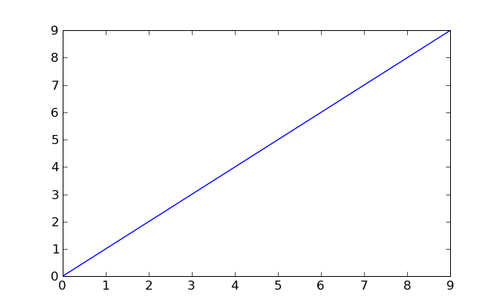
\includegraphics[width=10cm]{plot_x.png}\hfill}

Hemos creado un gráfico que representa diez puntos en un \emph{array} y luego lo hemos mostrado con \code{show()}; esto es así porque normalmente hacemos varios cambios en la gráfica antes de mostrarla, sin embargo, cuando trabajamos interactivamente, por ejemplo con la consola ipython podemos activar el \textbf{modo interactivo} para que cada cambio que se haga en la gráfica se muestre en el momento, mediante la función \textbf{ion()}, de esta menera no hace falta poner \code{show()} para mostrar la gráfica:

\begin{Verbatim}[commandchars=\\\{\}]
\PYG{g+gp}{\textgreater{}\textgreater{}\textgreater{} }\PYG{n}{ion}\PYG{p}{(}\PYG{p}{)}             \PYG{c}{\# Activo el modo interactivo}
\PYG{g+gp}{\textgreater{}\textgreater{}\textgreater{} }\PYG{n}{plot}\PYG{p}{(}\PYG{n}{x}\PYG{p}{)}           \PYG{c}{\# Hago un plot que se muestra sin hacer show()}
\PYG{g+gp}{\textgreater{}\textgreater{}\textgreater{} }\PYG{p}{[}\PYG{o}{\textless{}}\PYG{n}{matplotlib}\PYG{o}{.}\PYG{n}{lines}\PYG{o}{.}\PYG{n}{Line2D} \PYG{n+nb}{object} \PYG{n}{at} \PYG{l+m+mh}{0x9ffde8c}\PYG{o}{\textgreater{}}\PYG{p}{]}
\end{Verbatim}

Otra posibilidad es iniciar ipython en modo \code{pylab}, haciendo \code{ipython -pylab}, de esta manera se carga automáticamente pylab y se activa el modo interactivo, aparte de importar el módulo \code{numpy} y todas sus funciones.

Fíjate cómo el comando \code{plot()} devuelve una lista de instancias de cada dibujo. En este caso es una lista con un sólo elemento, una instancia \code{Line2D}. Podemos capturar esta instancia para referirnos a este dibujo más adelante haciendo:

\begin{Verbatim}[commandchars=\\\{\}]
\PYG{g+gp}{\textgreater{}\textgreater{}\textgreater{} }\PYG{n}{mi\PYGZus{}dibujo}\PYG{p}{,} \PYG{o}{=} \PYG{n}{plot}\PYG{p}{(}\PYG{n}{x}\PYG{p}{)}
\end{Verbatim}

Ahora la variable \code{mi\_dibujo} es una instancia o ``referencia'' a la línea del dibujo, que podremos manipular posteriormente con métodos que se aplican a esa instancia. Nótese que después de \code{mi\_dibujo} hay una coma; esto es para indicar que \code{mi\_dibujo} debe tomar el valor del primer (y en este caso el único) elemento de la lista y no la lista en sí, que es lo que habría ocurrido de haber hecho \code{mi\_dibujo = plot(x)} (erróneamente).

La sintaxis básica de \code{plot()} es simplemente \code{plot(x,y)()}, pero si no se incluye \code{x}, éste se reemplaza por el \textbf{número de elemento}, por lo que es equivalente a hacer \code{plot(range(len(y)),y)}. En la gráfica del ejemplo anterior no se ven diez puntos, sino una línea contínua uniendo esos puntos, que es como se dibuja por defecto. Si queremos pintar los puntos debemos hacerlo con un parámetro adicional, por ejemplo:

\begin{Verbatim}[commandchars=\\\{\}]
\PYG{g+gp}{\textgreater{}\textgreater{}\textgreater{} }\PYG{n}{plot}\PYG{p}{(}\PYG{n}{x}\PYG{p}{,}\PYG{l+s}{'}\PYG{l+s}{o}\PYG{l+s}{'}\PYG{p}{)}     \PYG{c}{\# Pinta diez puntos como "O"}
\PYG{g+gp}{\textgreater{}\textgreater{}\textgreater{} }\PYG{p}{[}\PYG{o}{\textless{}}\PYG{n}{matplotlib}\PYG{o}{.}\PYG{n}{lines}\PYG{o}{.}\PYG{n}{Line2D} \PYG{n+nb}{object} \PYG{n}{at} \PYG{l+m+mh}{0xa57ffac}\PYG{o}{\textgreater{}}\PYG{p}{]}

\PYG{g+gp}{\textgreater{}\textgreater{}\textgreater{} }\PYG{n}{plot}\PYG{p}{(}\PYG{n}{x}\PYG{p}{,}\PYG{l+s}{'}\PYG{l+s}{o-}\PYG{l+s}{'}\PYG{p}{)}    \PYG{c}{\# Igual que antes, pero uniéndolos además con una línea contínua}
\PYG{g+gp}{\textgreater{}\textgreater{}\textgreater{} }\PYG{p}{[}\PYG{o}{\textless{}}\PYG{n}{matplotlib}\PYG{o}{.}\PYG{n}{lines}\PYG{o}{.}\PYG{n}{Line2D} \PYG{n+nb}{object} \PYG{n}{at} \PYG{l+m+mh}{0xa58e80c}\PYG{o}{\textgreater{}}\PYG{p}{]}
\end{Verbatim}

{\hfill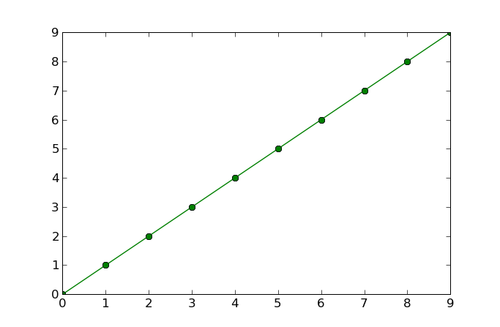
\includegraphics[width=10cm]{plot_xo.png}\hfill}

En este caso el \textbf{`o'} se usa para dibujar puntos gruesos y si se añade \textbf{-} también dibuja la línea contínua. En realidad se dibujaron dos gráficos uno encima del otro; si queremos que se cree un nuevo gráfico cada vez que hacemos \code{plot()}, debemos añadir el parámetro \code{hold=False} a  :func{}`plot(){}`:

\begin{Verbatim}[commandchars=\\\{\}]
\PYG{g+gp}{\textgreater{}\textgreater{}\textgreater{} }\PYG{n}{mi\PYGZus{}dibujo}\PYG{p}{,} \PYG{o}{=} \PYG{n}{plot}\PYG{p}{(}\PYG{n}{x}\PYG{o}{*}\PYG{l+m+mi}{2}\PYG{p}{,}\PYG{l+s}{'}\PYG{l+s}{o}\PYG{l+s}{'}\PYG{p}{,} \PYG{n}{hold}\PYG{o}{=}\PYG{l+s}{"}\PYG{l+s}{False}\PYG{l+s}{"}\PYG{p}{)}
\end{Verbatim}

El tercer parámetro (o segundo, si no se incluye la x) , donde se indica el símbolo y el color del marcador, admite distintas letras que representan de manera única el color, el símbolo o la línea que une los puntos; por ejemplo, si hacemos  \code{plot(x,'bx-')()} pintará los puntos con marcas ``X'', de color azul (`b') y los unirá además con líneas contínuas. Estas son otras opciones posibles:

\textbf{Marcas y líneas}

\begin{tabulary}{\linewidth}{|L|L|}
\hline
\textbf{
Símbolo
} & \textbf{
Descripción
}\\
\hline

`-`
 & 
Línea sólida
\\

`--`
 & 
Línea a trazos
\\

`-.'
 & 
Puntos y rayas
\\

`:'
 & 
Línea punteada
\\

`.'
 & 
Marcador punto
\\

`,'
 & 
Marcador pixel
\\

`o'
 & 
Marcador círculo relleno
\\

`v'
 & 
Marcador triángulo hacia abajo
\\

`\textasciicircum{}'
 & 
Marcador triángulo hacia arriba
\\

`\textless{}'
 & 
Marcador triángulo hacia la izquierda
\\

`\textgreater{}'
 & 
Marcador triángulo hacia la derecha
\\

`s'
 & 
Marcador cuadrado
\\

`p'
 & 
Marcador pentágono
\\

`*'
 & 
Marcador estrella
\\

`+'
 & 
Marcador cruz
\\

`x'
 & 
Marcador X
\\

`D'
 & 
Marcador diamante
\\

`d'
 & 
Marcador diamante delgado
\\
\hline
\end{tabulary}


\textbf{Colores}

\begin{tabulary}{\linewidth}{|L|L|}
\hline
\textbf{
Símbolo
} & \textbf{
Color
}\\
\hline

`b'
 & 
Azul
\\

`g'
 & 
Verde
\\

`r'
 & 
Rojo
\\

`c'
 & 
Cian
\\

`m'
 & 
Magenta
\\

`y'
 & 
Amarillo
\\

`k'
 & 
Negro
\\

`w'
 & 
Blanco
\\
\hline
\end{tabulary}


Para borrar toda la figura se puede usar la función  :func{}`clf(){}`, mientras que  \code{cla()} sólo borra lo que hay dibujado dentro de los ejes y no los ejes en si.

Se pueden representar varias \textbf{parejas de datos} con sus respectivos símbolos en una misma figura, aunque para ello siempre es obligatorio incluir el valor del eje x:

\begin{Verbatim}[commandchars=\\\{\}]
\PYG{g+gp}{\textgreater{}\textgreater{}\textgreater{} }\PYG{n}{clf}\PYG{p}{(}\PYG{p}{)}  \PYG{c}{\# Limpio la figura}
\PYG{g+gp}{\textgreater{}\textgreater{}\textgreater{} }\PYG{n}{x2} \PYG{o}{=} \PYG{n}{x}\PYG{o}{*}\PYG{o}{*}\PYG{l+m+mi}{2}
\PYG{g+gp}{\textgreater{}\textgreater{}\textgreater{} }\PYG{n}{x3} \PYG{o}{=} \PYG{n}{x}\PYG{o}{*}\PYG{o}{*}\PYG{l+m+mi}{3}

\PYG{g+gp}{\textgreater{}\textgreater{}\textgreater{} }\PYG{n}{plot}\PYG{p}{(}\PYG{n}{x}\PYG{p}{,} \PYG{n}{x}\PYG{p}{,}\PYG{l+s}{'}\PYG{l+s}{b.}\PYG{l+s}{'}\PYG{p}{,} \PYG{n}{x}\PYG{p}{,} \PYG{n}{x2}\PYG{p}{,} \PYG{l+s}{'}\PYG{l+s}{rd}\PYG{l+s}{'}\PYG{p}{,} \PYG{n}{x}\PYG{p}{,} \PYG{n}{x3}\PYG{p}{,} \PYG{l+s}{'}\PYG{l+s}{g\PYGZca{}}\PYG{l+s}{'}\PYG{p}{)}
\PYG{g+go}{\textgreater{}\textgreater{}\textgreater{}}
\PYG{g+go}{[\textless{}matplotlib.lines.Line2D object at 0xa94cf6c\textgreater{},}
\PYG{g+go}{\textless{}matplotlib.lines.Line2D object at 0xa95b72c\textgreater{},}
\PYG{g+go}{\textless{}matplotlib.lines.Line2D object at 0xa95ba4c\textgreater{}]}
\end{Verbatim}

{\hfill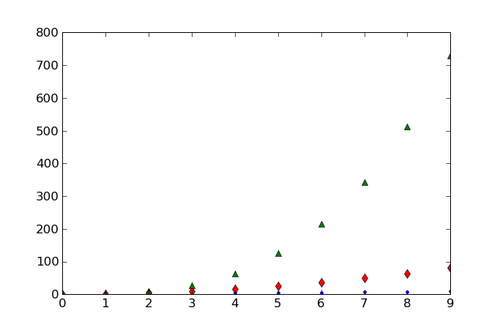
\includegraphics[width=10cm]{plot_x_x2_x3.png}\hfill}

Es posible cambiar el intervalo mostrado en los ejes con :func{}`xlim(){}`  e :func{}`ylim(){}`:

\begin{Verbatim}[commandchars=\\\{\}]
\PYG{g+gp}{\textgreater{}\textgreater{}\textgreater{} }\PYG{n}{xlim}\PYG{p}{(}\PYG{o}{-}\PYG{l+m+mi}{1}\PYG{p}{,}\PYG{l+m+mi}{11}\PYG{p}{)}   \PYG{c}{\# nuevos límites del eje x}
\PYG{g+gp}{\textgreater{}\textgreater{}\textgreater{} }\PYG{p}{(}\PYG{o}{-}\PYG{l+m+mi}{1}\PYG{p}{,} \PYG{l+m+mi}{11}\PYG{p}{)}
\PYG{g+gp}{\textgreater{}\textgreater{}\textgreater{} }\PYG{n}{ylim}\PYG{p}{(}\PYG{o}{-}\PYG{l+m+mi}{50}\PYG{p}{,}\PYG{l+m+mi}{850}\PYG{p}{)} \PYG{c}{\# nuevos límites del eje y}
\PYG{g+gp}{\textgreater{}\textgreater{}\textgreater{} }\PYG{p}{(}\PYG{o}{-}\PYG{l+m+mi}{50}\PYG{p}{,} \PYG{l+m+mi}{850}\PYG{p}{)}
\end{Verbatim}

además del marcador y el color indicado de la manera anterior, se pueden cambiar muchas otras propiedades de la gráfica como parámetros de \code{plot()} independientes:

\begin{tabulary}{\linewidth}{|L|L|}
\hline
\textbf{
Parámetro
} & \textbf{
Valores
}\\
\hline

alpha
 & 
float (0.0=transparente a 1.0=opaco)
\\

color o c
 & 
Un color de matplotlib
\\

label
 & 
string (cadena de texto)
\\

markeredgecolor o mec
 & 
Un color de matplotlib
\\

markeredgewidth o mew
 & 
float en puntos
\\

markerfacecolor o mfc
 & 
Un color de matplotlib
\\

markersize o ms float
 & 
float en puntos
\\

linestyle o ls
 & 
`-`  `--`  `-.'  `:'  `None'
\\

linewidth o lw
 & 
float en puntos
\\

marker
 & 
`+'  `*'  `,'  `.'  `1'  `2'  `3'  `4'
`\textless{}'  `\textgreater{}'  `D'  `H'  `\textasciicircum{}'  `\_' `d' `h'  `o'
`p'  `s'  `v'  `x'  `\textbar{}' TICKUP  TICKDOWN
TICKLEFT  TICKRIGHT
\\
\hline
\end{tabulary}


Un ejemplo usando más opciones sería este:

\begin{Verbatim}[commandchars=\\\{\}]
\PYG{g+gp}{\textgreater{}\textgreater{}\textgreater{} }\PYG{n}{plot}\PYG{p}{(}\PYG{n}{x}\PYG{p}{,} \PYG{n}{lw}\PYG{o}{=}\PYG{l+s}{'}\PYG{l+s}{5}\PYG{l+s}{'}\PYG{p}{,} \PYG{n}{c}\PYG{o}{=}\PYG{l+s}{'}\PYG{l+s}{y}\PYG{l+s}{'}\PYG{p}{,} \PYG{n}{marker}\PYG{o}{=}\PYG{l+s}{'}\PYG{l+s}{o}\PYG{l+s}{'}\PYG{p}{,} \PYG{n}{ms}\PYG{o}{=}\PYG{l+m+mi}{10}\PYG{p}{,} \PYG{n}{mfc}\PYG{o}{=}\PYG{l+s}{'}\PYG{l+s}{red}\PYG{l+s}{'}\PYG{p}{)}
\end{Verbatim}

{\hfill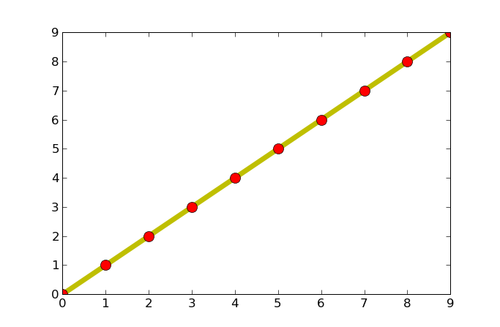
\includegraphics[width=10cm]{plot_x_markers.png}\hfill}

También es posible cambiar las propiedades de la gráfica una vez creada, para ello debemos \textbf{capturar las instancias} de cada dibujo en una variable y cambiar sus parámetros. En este caso a menudo hay que usar \code{show()} para actualizar el gráfico.:

\begin{Verbatim}[commandchars=\\\{\}]
\PYG{g+gp}{\textgreater{}\textgreater{}\textgreater{} }\PYG{n}{p1}\PYG{p}{,} \PYG{n}{p2}\PYG{p}{,} \PYG{n}{p3} \PYG{o}{=} \PYG{n}{plot}\PYG{p}{(}\PYG{n}{x}\PYG{p}{,} \PYG{n}{x}\PYG{p}{,}\PYG{l+s}{'}\PYG{l+s}{b.}\PYG{l+s}{'}\PYG{p}{,}   \PYG{c}{\# Hago tres dibujos, campturando sus}
\PYG{g+go}{            x, x2, 'rd', x, x3, 'g\PYGZca{}')   \#  instacias en las variables p1, p2 y p3}
\PYG{g+gp}{\textgreater{}\textgreater{}\textgreater{} }\PYG{n}{p1}\PYG{o}{.}\PYG{n}{set\PYGZus{}marker}\PYG{p}{(}\PYG{l+s}{'}\PYG{l+s}{o}\PYG{l+s}{'}\PYG{p}{)}             \PYG{c}{\# Cambio el símbolo de la gráfica 1}
\PYG{g+gp}{\textgreater{}\textgreater{}\textgreater{} }\PYG{n}{p3}\PYG{o}{.}\PYG{n}{set\PYGZus{}color}\PYG{p}{(}\PYG{l+s}{'}\PYG{l+s}{y}\PYG{l+s}{'}\PYG{p}{)}              \PYG{c}{\# Cambio el color de la gráfica 3}
\PYG{g+gp}{\textgreater{}\textgreater{}\textgreater{} }\PYG{n}{show}\PYG{p}{(}\PYG{p}{)}                         \PYG{c}{\# Muestro en dibujo por pantalla}
\end{Verbatim}


\section{Trabajando con texto}
\label{graficos:trabajando-con-texto}
Exiten funciones para añadir texto a los ejes y a la gráfica en sí, éstos son los más importantes:

\begin{Verbatim}[commandchars=\\\{\}]
\PYG{g+gp}{\textgreater{}\textgreater{}\textgreater{} }\PYG{n}{p1}\PYG{p}{,} \PYG{n}{p2}\PYG{p}{,} \PYG{n}{p3} \PYG{o}{=} \PYG{n}{plot}\PYG{p}{(}\PYG{n}{x}\PYG{p}{,} \PYG{n}{x}\PYG{p}{,} \PYG{n}{x}\PYG{p}{,} \PYG{n}{x2}\PYG{p}{,} \PYG{n}{x}\PYG{p}{,} \PYG{n}{x3}\PYG{p}{)}

\PYG{g+gp}{\textgreater{}\textgreater{}\textgreater{} }\PYG{n}{xlabel}\PYG{p}{(}\PYG{l+s}{'}\PYG{l+s}{Eje X}\PYG{l+s}{'}\PYG{p}{)}       \PYG{c}{\# Etiqueta del eje X}
\PYG{g+gp}{\textgreater{}\textgreater{}\textgreater{} }\PYG{o}{\textless{}}\PYG{n}{matplotlib}\PYG{o}{.}\PYG{n}{text}\PYG{o}{.}\PYG{n}{Text} \PYG{n+nb}{object} \PYG{n}{at} \PYG{l+m+mh}{0xad2d4ac}\PYG{o}{\textgreater{}}

\PYG{g+gp}{\textgreater{}\textgreater{}\textgreater{} }\PYG{n}{ylabel}\PYG{p}{(}\PYG{l+s}{'}\PYG{l+s}{Eje Y}\PYG{l+s}{'}\PYG{p}{)}       \PYG{c}{\# Etiqueta del eje Y}
\PYG{g+gp}{\textgreater{}\textgreater{}\textgreater{} }\PYG{o}{\textless{}}\PYG{n}{matplotlib}\PYG{o}{.}\PYG{n}{text}\PYG{o}{.}\PYG{n}{Text} \PYG{n+nb}{object} \PYG{n}{at} \PYG{l+m+mh}{0xad328cc}\PYG{o}{\textgreater{}}

\PYG{g+gp}{\textgreater{}\textgreater{}\textgreater{} }\PYG{n}{title}\PYG{p}{(}\PYG{l+s}{'}\PYG{l+s}{Mi grafica}\PYG{l+s}{'}\PYG{p}{)}   \PYG{c}{\# Título del gráfico}
\PYG{g+gp}{\textgreater{}\textgreater{}\textgreater{} }\PYG{o}{\textless{}}\PYG{n}{matplotlib}\PYG{o}{.}\PYG{n}{text}\PYG{o}{.}\PYG{n}{Text} \PYG{n+nb}{object} \PYG{n}{at} \PYG{l+m+mh}{0xad394ac}\PYG{o}{\textgreater{}}

\PYG{g+gp}{\textgreater{}\textgreater{}\textgreater{} }\PYG{n}{text}\PYG{p}{(}\PYG{l+m+mi}{7}\PYG{p}{,} \PYG{l+m+mi}{200}\PYG{p}{,} \PYG{l+s}{'}\PYG{l+s}{Nota}\PYG{l+s}{'}\PYG{p}{)}  \PYG{c}{\# Texto en coodenadas (7,200)}
\PYG{g+gp}{\textgreater{}\textgreater{}\textgreater{} }\PYG{o}{\textless{}}\PYG{n}{matplotlib}\PYG{o}{.}\PYG{n}{text}\PYG{o}{.}\PYG{n}{Text} \PYG{n+nb}{object} \PYG{n}{at} \PYG{l+m+mh}{0xa987e2c}\PYG{o}{\textgreater{}}
\end{Verbatim}

En este ejemplo, se usó la función \textbf{text()} para añadir un texto arbitrario en la gráfica, cuya posición se debe dar en \textbf{las unidades de la gráfica}. Cuando se utilizan textos también es posible usar fórmulas con formato LaTeX. Veamos un ejemplo:

\begin{Verbatim}[commandchars=\\\{\}]
\PYG{g+gp}{\textgreater{}\textgreater{}\textgreater{} }\PYG{n}{x} \PYG{o}{=} \PYG{n}{arange}\PYG{p}{(}\PYG{l+m+mi}{0}\PYG{p}{,} \PYG{l+m+mi}{6}\PYG{o}{*}\PYG{n}{pi}\PYG{p}{,}\PYG{l+m+mf}{0.1}\PYG{p}{)}

\PYG{g+gp}{\textgreater{}\textgreater{}\textgreater{} }\PYG{n}{y1} \PYG{o}{=} \PYG{n}{sin}\PYG{p}{(}\PYG{n}{x}\PYG{p}{)}\PYG{o}{/}\PYG{n}{x}
\PYG{g+gp}{\textgreater{}\textgreater{}\textgreater{} }\PYG{n}{y2} \PYG{o}{=} \PYG{n}{sin}\PYG{p}{(}\PYG{n}{x}\PYG{p}{)}\PYG{o}{*}\PYG{n}{exp}\PYG{p}{(}\PYG{o}{-}\PYG{n}{x}\PYG{p}{)}

\PYG{g+gp}{\textgreater{}\textgreater{}\textgreater{} }\PYG{n}{p1}\PYG{p}{,} \PYG{n}{p2} \PYG{o}{=} \PYG{n}{plot}\PYG{p}{(}\PYG{n}{x}\PYG{p}{,} \PYG{n}{y1}\PYG{p}{,} \PYG{n}{x}\PYG{p}{,} \PYG{n}{y2}\PYG{p}{)}

\PYG{g+gp}{\textgreater{}\textgreater{}\textgreater{} }\PYG{n}{texto1} \PYG{o}{=} \PYG{n}{text}\PYG{p}{(}\PYG{l+m+mi}{2}\PYG{p}{,} \PYG{l+m+mf}{0.6}\PYG{p}{,} \PYG{l+s}{r'}\PYG{l+s}{\$}\PYG{l+s}{\PYGZbs{}}\PYG{l+s}{frac\PYGZob{}}\PYG{l+s}{\PYGZbs{}}\PYG{l+s}{sin(x)\PYGZcb{}\PYGZob{}x\PYGZcb{}\$}\PYG{l+s}{'}\PYG{p}{,} \PYG{n}{fontsize}\PYG{o}{=}\PYG{l+m+mi}{20}\PYG{p}{)}
\PYG{g+gp}{\textgreater{}\textgreater{}\textgreater{} }\PYG{n}{texto2} \PYG{o}{=} \PYG{n}{text}\PYG{p}{(}\PYG{l+m+mi}{13}\PYG{p}{,} \PYG{l+m+mf}{0.2}\PYG{p}{,} \PYG{l+s}{r'}\PYG{l+s}{\$}\PYG{l+s}{\PYGZbs{}}\PYG{l+s}{sin(x) e\PYGZca{}\PYGZob{}x\PYGZcb{}\$}\PYG{l+s}{'}\PYG{p}{,} \PYG{n}{fontsize}\PYG{o}{=}\PYG{l+m+mi}{16}\PYG{p}{)}

\PYG{g+gp}{\textgreater{}\textgreater{}\textgreater{} }\PYG{n}{grid}\PYG{p}{(}\PYG{p}{)}       \PYG{c}{\# Añado una malla al gráfico}
\end{Verbatim}

Aquí hemos usado código LaTeX para escribir fórmulas matemáticas, para lo que siempre hay que escribir entre \code{r'\$ formula \$'} y he usado un tamaño de letra mayor con el parámetro \textbf{fontsize}. En la última línea hemos añadido una malla con la función \code{grid()}.

\begin{notice}{note}{Nota:}
LaTeX es un sistema de escritura orientado a contenidos matemáticos muy popular en ciencia e ingeniería. Puedes ver una introdución a LaTeX en los cursos ISLA de la ULL: \href{http://cisla.osl.ull.es/octubre06/htc/apuntes/latex}{http://cisla.osl.ull.es/octubre06/htc/apuntes/latex}
\end{notice}


\section{Representación gráfica de funciones}
\label{graficos:representacion-grafica-de-funciones}
Visto el ejemplo anterior, vemos que es muy fácil representar gráficamente una función matemática. Para ello, debemos definir la función y luego generar un \emph{array} con el intervalo de valores que se quieren representar. Definamos algunas funciones trigonométricas y luego representémolas gráficamente:

\begin{Verbatim}[commandchars=\\\{\}]
\PYG{g+gp}{\textgreater{}\textgreater{}\textgreater{} }\PYG{k}{def} \PYG{n+nf}{f1}\PYG{p}{(}\PYG{n}{x}\PYG{p}{)}\PYG{p}{:}
\PYG{g+go}{.....:     y = sin(x)}
\PYG{g+go}{.....:     return y}
\PYG{g+go}{.....:}

\PYG{g+gp}{\textgreater{}\textgreater{}\textgreater{} }\PYG{k}{def} \PYG{n+nf}{f2}\PYG{p}{(}\PYG{n}{x}\PYG{p}{)}\PYG{p}{:}
\PYG{g+go}{.....:     y = sin(x)+sin(5.0*x)}
\PYG{g+go}{.....:     return y}
\PYG{g+go}{.....:}

\PYG{g+gp}{\textgreater{}\textgreater{}\textgreater{} }\PYG{k}{def} \PYG{n+nf}{f3}\PYG{p}{(}\PYG{n}{x}\PYG{p}{)}\PYG{p}{:}
\PYG{g+go}{.....:     y = sin(x)*exp(-x/10.)}
\PYG{g+go}{.....:     return y}
\PYG{g+go}{.....:}

\PYG{g+gp}{\textgreater{}\textgreater{}\textgreater{} }\PYG{c}{\# array de valores que quiero representar}
\PYG{g+gp}{\textgreater{}\textgreater{}\textgreater{} }\PYG{n}{x} \PYG{o}{=} \PYG{n}{arange}\PYG{p}{(}\PYG{l+m+mi}{0}\PYG{p}{,} \PYG{l+m+mi}{10}\PYG{o}{*}\PYG{n}{pi}\PYG{p}{,} \PYG{l+m+mf}{0.1}\PYG{p}{)}

\PYG{g+gp}{\textgreater{}\textgreater{}\textgreater{} }\PYG{n}{p1}\PYG{p}{,} \PYG{n}{p2}\PYG{p}{,} \PYG{n}{p3} \PYG{o}{=} \PYG{n}{plot}\PYG{p}{(}\PYG{n}{x}\PYG{p}{,} \PYG{n}{f1}\PYG{p}{(}\PYG{n}{x}\PYG{p}{)}\PYG{p}{,} \PYG{n}{x}\PYG{p}{,} \PYG{n}{f2}\PYG{p}{(}\PYG{n}{x}\PYG{p}{)}\PYG{p}{,} \PYG{n}{x}\PYG{p}{,} \PYG{n}{f3}\PYG{p}{(}\PYG{n}{x}\PYG{p}{)}\PYG{p}{)}

\PYG{g+gp}{\textgreater{}\textgreater{}\textgreater{} }\PYG{c}{\# Añado una leyenda al gráfico}
\PYG{g+gp}{\textgreater{}\textgreater{}\textgreater{} }\PYG{n}{legend}\PYG{p}{(} \PYG{p}{(}\PYG{l+s}{'}\PYG{l+s}{Funcion 1}\PYG{l+s}{'}\PYG{p}{,} \PYG{l+s}{'}\PYG{l+s}{Funcion 2}\PYG{l+s}{'}\PYG{p}{,} \PYG{l+s}{'}\PYG{l+s}{Funcion 3}\PYG{l+s}{'}\PYG{p}{)} \PYG{p}{)}
\PYG{g+gp}{\textgreater{}\textgreater{}\textgreater{} }\PYG{o}{\textless{}}\PYG{n}{matplotlib}\PYG{o}{.}\PYG{n}{legend}\PYG{o}{.}\PYG{n}{Legend} \PYG{n+nb}{object} \PYG{n}{at} \PYG{l+m+mh}{0xbb4b0ac}\PYG{o}{\textgreater{}}
\end{Verbatim}

{\hfill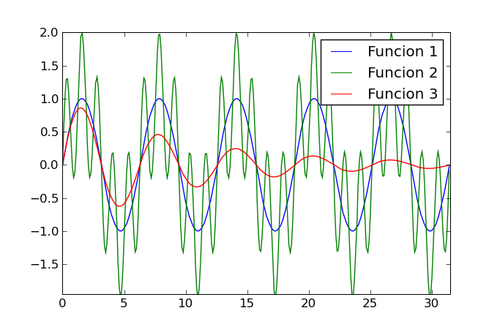
\includegraphics[width=10cm]{plot_funciones.png}\hfill}

En la última línea hemos añadido una leyenda con la función \code{legend()} que admite como entrada una \textbf{tupla} con \emph{strings} correspondiendo consecutivamente a cada uno de los gráficos.


\section{Histogramas}
\label{graficos:histogramas}
Los histogramas son gráficos que representan el número que veces que se repite ciertos valores dentro de un intervalo, frente a su valor. Podemos hacer histogramas muy fácilmente con la función \code{hist()} indicando como parámetros un \emph{array} con los números a representar. Si no se indica nada mas, se generará un histograma con 10 divisiones (llamadas \emph{bins}, en inglés). Veamos un ejemplo:

\begin{Verbatim}[commandchars=\\\{\}]
\PYG{g+gp}{\textgreater{}\textgreater{}\textgreater{} }\PYG{c}{\# Importo el módulo de numeros aleatorios de scipy}
\PYG{g+gp}{\textgreater{}\textgreater{}\textgreater{} }\PYG{k+kn}{from} \PYG{n+nn}{scipy} \PYG{k+kn}{import} \PYG{n}{random}
\PYG{g+gp}{\textgreater{}\textgreater{}\textgreater{} }\PYG{c}{\# utilizo la función randn() del modulo random para generar}
\PYG{g+gp}{\textgreater{}\textgreater{}\textgreater{} }\PYG{c}{\# un array de números aleatorios con distribución normal}
\PYG{g+gp}{\textgreater{}\textgreater{}\textgreater{} }\PYG{n}{nums} \PYG{o}{=} \PYG{n}{random}\PYG{o}{.}\PYG{n}{randn}\PYG{p}{(}\PYG{l+m+mi}{200}\PYG{p}{)}  \PYG{c}{\# array con 200 números aleatorios}
\PYG{g+gp}{\textgreater{}\textgreater{}\textgreater{} }\PYG{c}{\# Genero el histograma}
\PYG{g+gp}{\textgreater{}\textgreater{}\textgreater{} }\PYG{n}{hist}\PYG{p}{(}\PYG{n}{nums}\PYG{p}{)}
\PYG{g+go}{\textgreater{}\textgreater{}\textgreater{}}
\PYG{g+go}{(array([ 2, 10, 11, 28, 40, 49, 37, 12,  6,  5]),}
\PYG{g+go}{array([-2.98768497, -2.41750815, -1.84733134, -1.27715452, -0.70697771,}
\PYG{g+go}{        -0.13680089,  0.43337593,  1.00355274,  1.57372956,  2.14390637,}
\PYG{g+go}{        2.71408319]),}
\PYG{g+go}{\textless{}a list of 10 Patch objects\textgreater{})}
\end{Verbatim}

Vemos que los números del \emph{array} se dividieron automáticamente en 10 grupos (o \emph{bins}) y cada barra representa cada una de esas divisiones, con el número de valores que caen en cada intervalo. Si en lugar usar sólo 10 divisiones queremos usae digamos 20, debemos indicarlo como un segundo parámetro:

\begin{Verbatim}[commandchars=\\\{\}]
\PYG{g+gp}{\textgreater{}\textgreater{}\textgreater{} }\PYG{n}{hist}\PYG{p}{(}\PYG{n}{nums}\PYG{p}{,} \PYG{n}{bins}\PYG{o}{=}\PYG{l+m+mi}{20}\PYG{p}{)}
\end{Verbatim}

El la figura de abajo se muestra el resultado de superponer ambos histogramas. La función \code{hist()} devuelve una tupla con tres elementos, que son un array con el número elementos en cada división, un array con el punto en eje \emph{X} donde empieza cada división y una lista con referencias a cada una de las barras para modificar sus propiedades (consulta el manual de \code{matplotlib} para más información).

{\hfill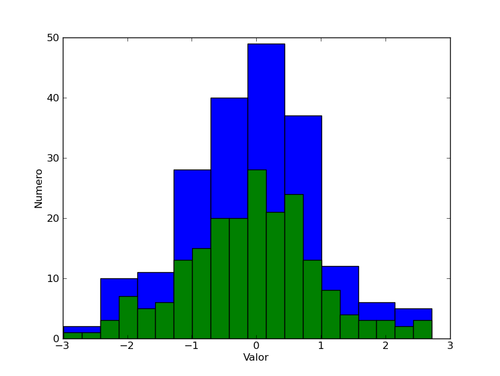
\includegraphics[width=10cm]{plot_histograma.png}\hfill}


\section{Figuras múltiples}
\label{graficos:figuras-multiples}
Se pueden hacer cuantas figuras independientes (en ventanas distintas) queramos con la función \code{figure(n)()} donde \emph{n} es el número de la figura. Cuando se crea una figura al hacer \code{plot()} se hace automáticamente \code{figure(1)()}, como aparece en el título de la ventana. Podríamos crear una nueva figura independiente excribiendo \code{figure(2)**, en ese momento todos los comandos de aplican a figura activa, la figura 2. Podemos regresar a la primera excribiendo :func:{}`figure(1)()} para trabajar nuevamente en ella.:

\begin{Verbatim}[commandchars=\\\{\}]
\PYG{g+gp}{\textgreater{}\textgreater{}\textgreater{} }\PYG{n}{p1}\PYG{p}{,} \PYG{o}{=} \PYG{n}{plot}\PYG{p}{(}\PYG{n}{sin}\PYG{p}{(}\PYG{n}{x}\PYG{p}{)}\PYG{p}{)}             \PYG{c}{\# Crea una figura en una ventana (Figure 1)}
\PYG{g+gp}{\textgreater{}\textgreater{}\textgreater{} }\PYG{n}{figure}\PYG{p}{(}\PYG{l+m+mi}{2}\PYG{p}{)}                \PYG{c}{\# Crea una nueva figura (vacía) en otra ventana (Figure 2)}
\PYG{g+gp}{\textgreater{}\textgreater{}\textgreater{} }\PYG{n}{p2}\PYG{p}{,} \PYG{o}{=} \PYG{n}{plot}\PYG{p}{(}\PYG{n}{cos}\PYG{p}{(}\PYG{n}{x}\PYG{p}{)}\PYG{p}{)}             \PYG{c}{\# Dibuja el gráfico en la figura 2}
\PYG{g+gp}{\textgreater{}\textgreater{}\textgreater{} }\PYG{n}{title}\PYG{p}{(}\PYG{l+s}{'}\PYG{l+s}{Funcion coseno}\PYG{l+s}{'}\PYG{p}{)}  \PYG{c}{\# Añade un título a la figura 2}
\PYG{g+gp}{\textgreater{}\textgreater{}\textgreater{} }\PYG{n}{figure}\PYG{p}{(}\PYG{l+m+mi}{1}\PYG{p}{)}                \PYG{c}{\# Activo la figura 1}
\PYG{g+gp}{\textgreater{}\textgreater{}\textgreater{} }\PYG{n}{title}\PYG{p}{(}\PYG{l+s}{'}\PYG{l+s}{Funcion seno}\PYG{l+s}{'}\PYG{p}{)}    \PYG{c}{\# Añade un título a la figura 2}
\end{Verbatim}


\section{Varios gráficos en una figura}
\label{graficos:varios-graficos-en-una-figura}
En ocasiones nos interesa mostrar varios gráficos en un misma figura o ventana. Para ello podemos usar la función \code{subplot()}, indicando entre paréntesis un número con tres dígitos cuyo primer dígito indica en número de filas en los que se dividirá la figura, el segundo el número de columnas y el tercero se refiere al gráfico con el que estamos trabajando en ese momento. Por ejemplo, si quisiéramos representar las tres funciones anteriores usando tres gráficas en la misma figura, una al lado de la otra y por lo tanto con una fila y tres columnas, haríamos lo siguiente:

\begin{Verbatim}[commandchars=\\\{\}]
\PYG{g+gp}{\textgreater{}\textgreater{}\textgreater{} }\PYG{n}{subplot}\PYG{p}{(}\PYG{l+m+mi}{131}\PYG{p}{)}      \PYG{c}{\# Figura con una fila y tres columnas, activo primer subgráfico}
\PYG{g+gp}{\textgreater{}\textgreater{}\textgreater{} }\PYG{n}{p1}\PYG{p}{,} \PYG{o}{=} \PYG{n}{plot}\PYG{p}{(}\PYG{n}{x}\PYG{p}{,}\PYG{n}{f1}\PYG{p}{(}\PYG{n}{x}\PYG{p}{)}\PYG{p}{,}\PYG{l+s}{'}\PYG{l+s}{r-}\PYG{l+s}{'}\PYG{p}{)}

\PYG{g+gp}{\textgreater{}\textgreater{}\textgreater{} }\PYG{n}{subplot}\PYG{p}{(}\PYG{l+m+mi}{132}\PYG{p}{)}      \PYG{c}{\# Figura con una fila y tres columnas, activo segundo subgráfico}
\PYG{g+gp}{\textgreater{}\textgreater{}\textgreater{} }\PYG{n}{p2}\PYG{p}{,} \PYG{o}{=} \PYG{n}{plot}\PYG{p}{(}\PYG{n}{x}\PYG{p}{,}\PYG{n}{f2}\PYG{p}{(}\PYG{n}{x}\PYG{p}{)}\PYG{p}{,}\PYG{l+s}{'}\PYG{l+s}{b-}\PYG{l+s}{'}\PYG{p}{)}

\PYG{g+gp}{\textgreater{}\textgreater{}\textgreater{} }\PYG{n}{subplot}\PYG{p}{(}\PYG{l+m+mi}{133}\PYG{p}{)}      \PYG{c}{\# Figura con una fila y tres columnas, activo tercer subgráfico}
\PYG{g+gp}{\textgreater{}\textgreater{}\textgreater{} }\PYG{n}{p3}\PYG{p}{,} \PYG{o}{=} \PYG{n}{plot}\PYG{p}{(}\PYG{n}{x}\PYG{p}{,}\PYG{n}{f3}\PYG{p}{(}\PYG{n}{x}\PYG{p}{)}\PYG{p}{,}\PYG{l+s}{'}\PYG{l+s}{g-}\PYG{l+s}{'}\PYG{p}{)}
\end{Verbatim}

{\hfill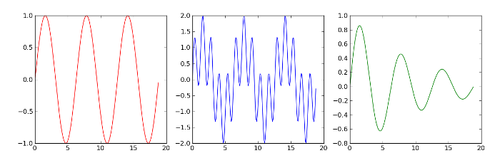
\includegraphics{plot_subplot.png}\hfill}

Al igual que con varias figuras, para dibujar en un gráfico hay que activarlo, así, si acabamos de dibujar el segundo gráfico escribiendo antes \textbf{subplot(132)} y queremos cambiar algo del primero, debemos activarlo con \code{subplot(131)()} y en ese momento todas funciones de gráficas se aplicarán a él.


\section{Representando datos de laboratorio}
\label{graficos:representando-datos-de-laboratorio}
Representar datos leídos de un fichero en lugar de generarlos directamente, es tan fácil como leer los datos y pasar los a \emph{arrays} de numpy. Una vez hecho, se grafican como hemos visto:

\begin{Verbatim}[commandchars=\\\{\}]
\PYG{g+gp}{\textgreater{}\textgreater{}\textgreater{} }\PYG{c}{\# Leo un fichero de dos columnas de datos, pasándolo a un array}
\PYG{g+gp}{\textgreater{}\textgreater{}\textgreater{} }\PYG{n}{datos} \PYG{o}{=} \PYG{n}{loadtxt}\PYG{p}{(}\PYG{l+s}{'}\PYG{l+s}{datos\PYGZus{}2col.txt}\PYG{l+s}{'}\PYG{p}{)}
\PYG{g+gp}{\textgreater{}\textgreater{}\textgreater{} }\PYG{n}{datos}\PYG{o}{.}\PYG{n}{shape}   \PYG{c}{\# 100 filas, 2 columnas}
\PYG{g+gp}{\textgreater{}\textgreater{}\textgreater{} }\PYG{p}{(}\PYG{l+m+mi}{100}\PYG{p}{,} \PYG{l+m+mi}{2}\PYG{p}{)}

\PYG{g+gp}{\textgreater{}\textgreater{}\textgreater{} }\PYG{n}{col2}\PYG{p}{,} \PYG{o}{=} \PYG{n}{plot}\PYG{p}{(}\PYG{n}{datos}\PYG{p}{[}\PYG{p}{:}\PYG{p}{,}\PYG{l+m+mi}{1}\PYG{p}{]}\PYG{p}{,} \PYG{l+s}{'}\PYG{l+s}{b.}\PYG{l+s}{'}\PYG{p}{)}   \PYG{c}{\# Primera columna, con puntos azules (b)}
\PYG{g+gp}{\textgreater{}\textgreater{}\textgreater{} }\PYG{n}{col1}\PYG{p}{,} \PYG{o}{=} \PYG{n}{plot}\PYG{p}{(}\PYG{n}{datos}\PYG{p}{[}\PYG{p}{:}\PYG{p}{,}\PYG{l+m+mi}{0}\PYG{p}{]}\PYG{p}{,} \PYG{l+s}{'}\PYG{l+s}{r.}\PYG{l+s}{'}\PYG{p}{)}   \PYG{c}{\# Segunda columna, con puntos rojos (r)}

\PYG{g+gp}{\textgreater{}\textgreater{}\textgreater{} }\PYG{c}{\# Trazo una línea horizontal en la coordenada y=4 de color verde (g)}
\PYG{g+gp}{\textgreater{}\textgreater{}\textgreater{} }\PYG{n}{axhline}\PYG{p}{(}\PYG{l+m+mi}{4}\PYG{p}{,} \PYG{n}{color}\PYG{o}{=}\PYG{l+s}{'}\PYG{l+s}{g}\PYG{l+s}{'}\PYG{p}{)}
\PYG{g+gp}{\textgreater{}\textgreater{}\textgreater{} }\PYG{o}{\textless{}}\PYG{n}{matplotlib}\PYG{o}{.}\PYG{n}{lines}\PYG{o}{.}\PYG{n}{Line2D} \PYG{n+nb}{object} \PYG{n}{at} \PYG{l+m+mh}{0x169c6d8c}\PYG{o}{\textgreater{}}

\PYG{g+gp}{\textgreater{}\textgreater{}\textgreater{} }\PYG{c}{\# Trazo una línea vertical en la coordenada x=30 de color verde (g)}
\PYG{g+gp}{\textgreater{}\textgreater{}\textgreater{} }\PYG{n}{axvline}\PYG{p}{(}\PYG{l+m+mi}{20}\PYG{p}{,} \PYG{n}{color}\PYG{o}{=}\PYG{l+s}{'}\PYG{l+s}{g}\PYG{l+s}{'}\PYG{p}{)}
\PYG{g+gp}{\textgreater{}\textgreater{}\textgreater{} }\PYG{o}{\textless{}}\PYG{n}{matplotlib}\PYG{o}{.}\PYG{n}{lines}\PYG{o}{.}\PYG{n}{Line2D} \PYG{n+nb}{object} \PYG{n}{at} \PYG{l+m+mh}{0xac5986c}\PYG{o}{\textgreater{}}

\PYG{g+gp}{\textgreater{}\textgreater{}\textgreater{} }\PYG{c}{\# Dibujo una banda horizontal de y=0 a y=2 de color azul y 30\% de transparencia (alpha=0.3)}
\PYG{g+gp}{\textgreater{}\textgreater{}\textgreater{} }\PYG{n}{axhspan}\PYG{p}{(}\PYG{l+m+mi}{0}\PYG{p}{,} \PYG{l+m+mi}{2}\PYG{p}{,} \PYG{n}{alpha}\PYG{o}{=}\PYG{l+m+mf}{0.3}\PYG{p}{,} \PYG{n}{color}\PYG{o}{=}\PYG{l+s}{'}\PYG{l+s}{b}\PYG{l+s}{'}\PYG{p}{)}
\PYG{g+gp}{\textgreater{}\textgreater{}\textgreater{} }\PYG{o}{\textless{}}\PYG{n}{matplotlib}\PYG{o}{.}\PYG{n}{patches}\PYG{o}{.}\PYG{n}{Polygon} \PYG{n+nb}{object} \PYG{n}{at} \PYG{l+m+mh}{0xac59c4c}\PYG{o}{\textgreater{}}

\PYG{g+gp}{\textgreater{}\textgreater{}\textgreater{} }\PYG{c}{\# Dibujo una banda vertical de x=60 a x=80 de color verde y 30\% de transparencia}
\PYG{g+gp}{\textgreater{}\textgreater{}\textgreater{} }\PYG{n}{axvspan}\PYG{p}{(}\PYG{l+m+mi}{60}\PYG{p}{,} \PYG{l+m+mi}{80}\PYG{p}{,} \PYG{n}{alpha}\PYG{o}{=}\PYG{l+m+mf}{0.3}\PYG{p}{,} \PYG{n}{color}\PYG{o}{=}\PYG{l+s}{'}\PYG{l+s}{g}\PYG{l+s}{'}\PYG{p}{)}
\PYG{g+gp}{\textgreater{}\textgreater{}\textgreater{} }\PYG{o}{\textless{}}\PYG{n}{matplotlib}\PYG{o}{.}\PYG{n}{patches}\PYG{o}{.}\PYG{n}{Polygon} \PYG{n+nb}{object} \PYG{n}{at} \PYG{l+m+mh}{0xac59a0c}\PYG{o}{\textgreater{}}

\PYG{g+gp}{\textgreater{}\textgreater{}\textgreater{} }\PYG{c}{\# Etiqueto los ejes}
\PYG{g+gp}{\textgreater{}\textgreater{}\textgreater{} }\PYG{n}{xlabel}\PYG{p}{(}\PYG{l+s}{'}\PYG{l+s}{Eje X}\PYG{l+s}{'}\PYG{p}{)}
\PYG{g+gp}{\textgreater{}\textgreater{}\textgreater{} }\PYG{o}{\textless{}}\PYG{n}{matplotlib}\PYG{o}{.}\PYG{n}{text}\PYG{o}{.}\PYG{n}{Text} \PYG{n+nb}{object} \PYG{n}{at} \PYG{l+m+mh}{0xad043ac}\PYG{o}{\textgreater{}}
\PYG{g+gp}{\textgreater{}\textgreater{}\textgreater{} }\PYG{n}{ylabel}\PYG{p}{(}\PYG{l+s}{'}\PYG{l+s}{Eje Y}\PYG{l+s}{'}\PYG{p}{)}
\PYG{g+gp}{\textgreater{}\textgreater{}\textgreater{} }\PYG{o}{\textless{}}\PYG{n}{matplotlib}\PYG{o}{.}\PYG{n}{text}\PYG{o}{.}\PYG{n}{Text} \PYG{n+nb}{object} \PYG{n}{at} \PYG{l+m+mh}{0xad0b52c}\PYG{o}{\textgreater{}}
\end{Verbatim}

En este caso hemos usado además algunas funciones para crear líneas y bandas horizontales y verticales.

{\hfill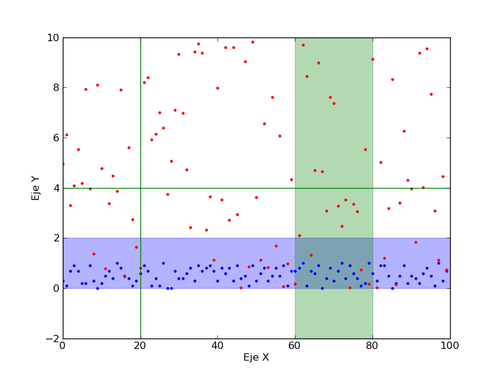
\includegraphics[width=10cm]{plot_labdata.png}\hfill}


\section{Barras de error}
\label{graficos:barras-de-error}
Cuando se trabaja con datos de laboratorio es muy habitual dibujar barras de error en los puntos representados. Esto se puede hacer usando la función \code{errorbar()} en lugar de \code{plot()} o junto con ella. Su sintáxis es similar, pero no igual, a la que hay que incluir los errores como parámetros usando \emph{floats} si son errores iguales para todos los puntos o bien un array representando el error de cada punto. Veamos un ejemplo:

\begin{Verbatim}[commandchars=\\\{\}]
\PYG{c}{\# Datos de x e y}
\PYG{n}{x} \PYG{o}{=} \PYG{n}{arange}\PYG{p}{(}\PYG{l+m+mf}{0.1}\PYG{p}{,} \PYG{l+m+mf}{5.0}\PYG{p}{,} \PYG{l+m+mf}{0.1}\PYG{p}{)}
\PYG{n}{y} \PYG{o}{=} \PYG{n}{exp}\PYG{p}{(}\PYG{o}{-}\PYG{n}{x}\PYG{p}{)}

\PYG{c}{\# Error constante en x e y}
\PYG{n}{err\PYGZus{}x} \PYG{o}{=} \PYG{l+m+mf}{0.1}
\PYG{n}{err\PYGZus{}y} \PYG{o}{=} \PYG{l+m+mf}{0.2}

\PYG{n}{errorbar}\PYG{p}{(}\PYG{n}{x}\PYG{p}{,} \PYG{n}{y}\PYG{p}{,} \PYG{n}{xerr}\PYG{o}{=}\PYG{n}{err\PYGZus{}x}\PYG{p}{,} \PYG{n}{yerr}\PYG{o}{=}\PYG{n}{err\PYGZus{}y}\PYG{p}{)}

\PYG{c}{\# Si los errores de x e y son distintos en cada}
\PYG{c}{\# punto, se ponen en un array}
\PYG{n}{err\PYGZus{}y} \PYG{o}{=} \PYG{l+m+mf}{0.1} \PYG{o}{+} \PYG{l+m+mf}{0.2}\PYG{o}{*}\PYG{n}{sqrt}\PYG{p}{(}\PYG{n}{x}\PYG{p}{)}
\PYG{n}{err\PYGZus{}x} \PYG{o}{=} \PYG{l+m+mf}{0.1} \PYG{o}{+} \PYG{n}{err\PYGZus{}y}

\PYG{c}{\# Gráfico con la barra de error en x e y, usando}
\PYG{c}{\# línea continua y puntos (fmt='-o')}
\PYG{n}{errorbar}\PYG{p}{(}\PYG{n}{x}\PYG{p}{,} \PYG{n}{y}\PYG{p}{,} \PYG{n}{xerr}\PYG{o}{=}\PYG{n}{err\PYGZus{}x}\PYG{p}{,} \PYG{n}{yerr}\PYG{o}{=}\PYG{n}{err\PYGZus{}y}\PYG{p}{,} \PYG{n}{fmt}\PYG{o}{=}\PYG{l+s}{'}\PYG{l+s}{-o}\PYG{l+s}{'}\PYG{p}{)}
\end{Verbatim}

{\hfill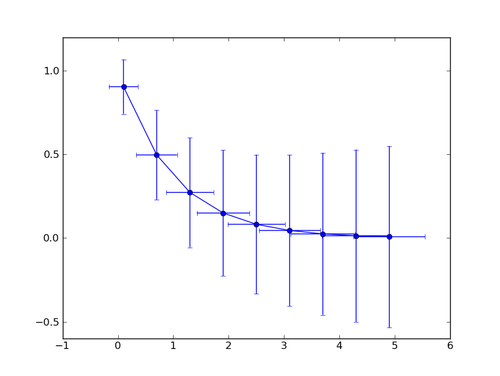
\includegraphics[width=10cm]{plot_errorbar.png}\hfill}

Para algunos tipos de datos, conviene representar alguno de los ejes o ambos en escala logarítmica para apreciar mejor la evolución de la gráfica. Podemos usar las funciones \textbf{semilogx()}, \textbf{semilogy()} o \textbf{loglog()} para hacer un gráfico en escala logarítmica en el eje x, y o ambos, respectivamente. Por ejemplo, para representar el gráfico anterior con el eje y en escala logarítmica, podemos hacer lo siguiente:

\begin{Verbatim}[commandchars=\\\{\}]
\PYG{c}{\# Eje y en escala logarítmica}
\PYG{n}{p1}\PYG{p}{,} \PYG{o}{=} \PYG{n}{semilogy}\PYG{p}{(}\PYG{n}{x}\PYG{p}{,} \PYG{n}{y}\PYG{p}{,}\PYG{l+s}{'}\PYG{l+s}{rs-}\PYG{l+s}{'}\PYG{p}{)}
\end{Verbatim}

{\hfill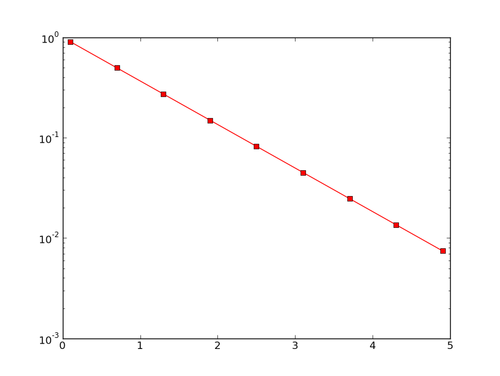
\includegraphics[width=10cm]{plot_semilogy.png}\hfill}


\section{Datos bidimensionales}
\label{graficos:datos-bidimensionales}
Es posible representar datos bidimensionales, como podría ser una imagen, usando la función \code{imshow()}:

\begin{Verbatim}[commandchars=\\\{\}]
\PYG{g+gp}{\textgreater{}\textgreater{}\textgreater{} }\PYG{c}{\# Creo un array 2D 100x100 de valores de 0.0 a 99999.0}
\PYG{g+gp}{\textgreater{}\textgreater{}\textgreater{} }\PYG{n}{datos2D} \PYG{o}{=} \PYG{n}{arange}\PYG{p}{(}\PYG{l+m+mf}{10000.}\PYG{p}{)}\PYG{o}{.}\PYG{n}{reshape}\PYG{p}{(}\PYG{l+m+mi}{100}\PYG{p}{,}\PYG{l+m+mi}{100}\PYG{p}{)}
\PYG{g+gp}{\textgreater{}\textgreater{}\textgreater{} }\PYG{n}{datos2D}\PYG{o}{.}\PYG{n}{shape}
\PYG{g+gp}{\textgreater{}\textgreater{}\textgreater{} }\PYG{p}{(}\PYG{l+m+mi}{100}\PYG{p}{,} \PYG{l+m+mi}{100}\PYG{p}{)}
\PYG{g+gp}{\textgreater{}\textgreater{}\textgreater{} }\PYG{c}{\# Gráfico del array bidimensional}
\PYG{g+gp}{\textgreater{}\textgreater{}\textgreater{} }\PYG{n}{imshow}\PYG{p}{(}\PYG{n}{datos2D}\PYG{p}{)}
\PYG{g+gp}{\textgreater{}\textgreater{}\textgreater{} }\PYG{c}{\# Añado una barra de color para indicar los nieveles}
\PYG{g+gp}{\textgreater{}\textgreater{}\textgreater{} }\PYG{n}{colorbar}\PYG{p}{(}\PYG{p}{)}
\PYG{g+gp}{\textgreater{}\textgreater{}\textgreater{} }\PYG{c}{\# Cambio a la paleta de colores gray() (por defecto es jet())}
\PYG{g+gp}{\textgreater{}\textgreater{}\textgreater{} }\PYG{n}{gray}\PYG{p}{(}\PYG{p}{)}
\end{Verbatim}

{\hfill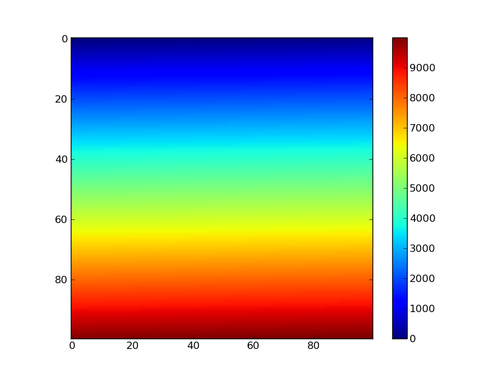
\includegraphics[width=10cm]{plot_datos2D.png}\hfill}


\section{Guardando las imágenes}
\label{graficos:guardando-las-imagenes}
Después de crear una imagen podemos guardarla con la función \code{savefig()} poniendo como parámetro el nombre del fichero con su extensión. El formato de grabado se toma automáticamente de la extensión del nombre. Los formatos disponibles son png, pdf, ps, eps y svg. Por ejemplo:

\begin{Verbatim}[commandchars=\\\{\}]
\PYG{g+gp}{\textgreater{}\textgreater{}\textgreater{} }\PYG{n}{savefig}\PYG{p}{(}\PYG{l+s}{"}\PYG{l+s}{mi\PYGZus{}primera\PYGZus{}grafica.eps}\PYG{l+s}{"}\PYG{p}{)}  \PYG{c}{\# Guardo la figura en formato eps}
\PYG{g+gp}{\textgreater{}\textgreater{}\textgreater{} }\PYG{n}{savefig}\PYG{p}{(}\PYG{l+s}{"}\PYG{l+s}{mi\PYGZus{}primera\PYGZus{}grafica.png}\PYG{l+s}{"}\PYG{p}{)}  \PYG{c}{\# Guardo la figura en formato png}
\end{Verbatim}

Si el gráfico se va usar para imprimir, por ejemplo en una publicación científica o en un informe, es recomendable usar un formato vectorial como Postcript (ps) o Postcript encapsulado (eps), pero si es para mostrar por pantalla o en una web, el más adecuado es un formato de mapa de bits como png o jpg.

Consulta la web de \textbf{matplotlib} (\href{http://matplotlib.sourceforge.net/}{http://matplotlib.sourceforge.net/}) para ver muchas más propiedades y ejemplos de esta librería.


\section{Ejercicios}
\label{graficos:ejercicios}\begin{enumerate}
\item {} 
Representar gráficamente las siguientes funciones:
\begin{quote}
\begin{gather}
\begin{split}f(x) = a e^{- { \frac{(x-x_0)^2 }{ 2 c^2} } }  \hspace{1cm}  f(x) =  \frac{b}{(x - x_0)^2 + b^2 }\end{split}\notag
\end{gather}\end{quote}

usando los valores \emph{a=2.0}, $x_0=10.0$, \emph{c=5,0} y \emph{b=0.5} en el intervalo x={[}-50,+50{]}.

\item {} 
Con la serie de Gregory-Leibniz para el cálculo $\pi$ usada anteriormente:
\begin{quote}
\begin{gather}
\begin{split}4 \sum^n_{k=1} \frac{(-1)^{k+1}}{2k - 1}\end{split}\notag
\end{gather}\end{quote}

el valor obtenido de  $\pi$ se acerca lentamenta al verdadero con cada término. Calcular todos los  valores que va tomando  $\pi$ con cada término hasta llegar a un error absoluto de  $10^{-6}$ y representa en una gráfica ese valor frente número de elementos sumados, usando líneas contínuas, limitándonos a los 300 primeros elementos. El otro gráfico representar el valor de  $\pi$ en los últimos 300 elementos. En gráficas dintintas, representar esta vez el valor abosuluto de la diferencia entre el valor calculado y el real frente al número de elementos, reprentando igualmente los 300 primeros en una gráfica y los 300 últimos en otra.

\item {} 
El fichero medidas\_I131.txt (tema 6 en el aula virtual) contiene medidas de masa de yodo 131 radioactivo hechas diariamente para medir su coeficiente de desintegración. La primera columna es la masa residual en gramos y la segunda es el error de la medida. Representar gráficamente los datos incluyendo barras de error usando puntos sin líneas, etiquetando los ejes.

\item {} 
Cuando una fuente de luz coherente atraviesa una rendija delgada, se produce difracción de la luz, cuyo patrón de intensidad en la aproximación de Fraunhofer está dado por:
\begin{quote}
\begin{gather}
\begin{split}I(\theta) = I_0(\frac{sen \beta}{\beta})^2 \hspace{3cm}  \beta = \frac{\pi a sen \theta}{\lambda}\end{split}\notag
\end{gather}\end{quote}

donde \emph{a} es el ancho de la rendija, $\lambda$ la longitud de onda de la luz,  $I_0$ la intensidad en el eje y $\theta$ el ángulo de la posición medida con el eje de la rendija (ver dibujo). Representar gráficamente la intensidad del patrón de difracción para  $\lambda=400nm$,  $\lambda=650nm$ y $\lambda=800nm$ usando  $I_0=1$ y \emph{a=0.04mm} en el intervalo  $-\pi/20 < \theta < +\pi/20$. Comprobar cual es el efecto del patrón de difracción al duplicar el ancho de la rendija.

{\hfill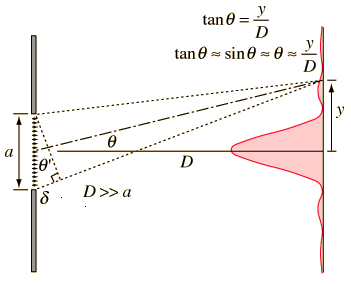
\includegraphics[width=7cm]{fraungeo.png}\hfill}

\item {} 
Como ya hemos visto, la variación de temperatura de un objeto a temperatura $T_0$ en un ambiente a $T_s$ cambia de la siguiente manera:
\begin{quote}
\begin{gather}
\begin{split}T =  T_s + (T_0 - T_s)e^{-kt}\end{split}\notag
\end{gather}\end{quote}

con $t$ en horas y \emph{k} un parámetro que depende del cuerpo. a) Representa gráficamente la variación de la temperatura con el tiempo, partiendo de una $T_0=5^\circ C$ a lo largo de 24 horas suponiendo \emph{k=0.45} y temperatura ambiente de 40ºC. b) Superpon sobre esta curva las curvas correspondientes a cuerpos con \emph{k=0.3} y \emph{k=0.6} con distinto color y trazado identificándolas con una leyenda.

\item {} 
Representa nuevamente la curva del apartado a) del ejercicio anterior superponiendo además las  curvas correspondientes a temperaturas iniciales distintas, de  $T_0=-5^\circ C$ y $T_0=15^\circ C$. Para $T_0=5^\circ C$ representa un una gráfica aparte cómo cambian las curvas con temperaturas ambiente de 20ºC y 50ºC, además de la de 40ºC. Identifica cada curva y etiqueta correctamente los ejes en todas las gráficas.

\item {} 
La curva plana llamada trocoide, una generalización de la cicloide, es la curva descrita por un punto P situado a una distancia \emph{b} del centro de una circunferencia de radio \emph{a}, a medida que rueda (sin deslizar) por una superficie horizontal. Tiene por coordenadas (x,y) las siguientes:
\begin{quote}
\begin{gather}
\begin{split}x = a \ \phi - b \ sen \phi \ \ \ ,\ \ \ y = a - b\ cos \phi\end{split}\notag
\end{gather}\end{quote}

Escribir un programa que dibuje tres curvas (contínuas y sin símbolos), en el mismo gráfico cartesiano (OX,OY), para un intervalo $\phi=[0.0,18.0]$ (en radianes) y para los valores de \emph{a=5.0} y \emph{b=2.0, 5.0 y 8.0} . Rotular apropiadamente los ejes e incluir una leyenda con los tres valores de  que distinguen las tres curvas.

\item {} 
El movimiento de oscilador amortiguado se puede expresar la siguiente manera:
\begin{quote}
\begin{gather}
\begin{split}x = A_0 e^{-k\omega t} \cos{(\omega t + \delta)}\end{split}\notag
\end{gather}\end{quote}

Siendo $A_0$ la amplitud inicial, $\omega$ la fecuencia de oscilación y \emph{k} el factor de amortiguamiento. Representar gráficamente el movimiento de un oscilador forzado de amplitud inicial de 10cm y frecuencia de 10 ciclos por segundo y $\delta=\pi/8$ con factores de amortiguamiento de 0.1, 0.4, 0.9 y 1.1.

Para el gráfico correspondiente a \emph{k=0.1} dibujar con líneas a trazos los valores máximos y mínimos del movimiento oscilatorio. Nótese corresponden a las curvas para las que $x=A_0$ y $x=-A_0$.

\end{enumerate}


\chapter{Ajuste de datos experimentales: Método de mínimos cuadrados}
\label{ajustes:ajuste-de-datos-experimentales-metodo-de-minimos-cuadrados}\label{ajustes::doc}
Un trabajo habitual de laboratorio es la creación de un modelo
matemático de cierto comportamiento físico empleando datos
experimentales. Por ejemplo, si se toman medidas de la amplitud de las oscilaciones de un
péndulo,  es posible obtener una función oscilatoria
analítica que describa ese movimiento con la frecuencia y amplitud
adecuadas para cualquier instante de tiempo.

Aunque existen muchas técnicas para el ajuste de funciones a datos
experimentales, el método más común es el de \emph{mínimos cuadrados}.
Supongamos que tenemos una serie de medidas $(x_1, y_1), (x_2,
y_2), (x_3, y_3), \dots , (x_n, y_n)$, siendo \emph{x} la variable
independiente e \emph{y} la dependiente. Para un modelo $f(x)$ de
estos datos, hay un error \emph{r} para cada medida de $r_1
= y_1 -f(x_1), r_2 = y_2 -f(x_2), \dots ,  r_n = y_n -f(x_n)$. Según
el método de mínimos cuadrados, la mejor función de ajuste \emph{f(x)} es
aquella en la que
\begin{gather}
\begin{split}R = d_1^2 + d_2^2 + \dots + d_n^2 = \sum^n_{i=1} d^2_i = \sum^n_{i=1}  \lvert y_i - f(x_i)\rvert\end{split}\notag
\end{gather}
es minimo. La forma canónica de este problema es
\begin{gather}
\begin{split}Xa = Y\end{split}\notag
\end{gather}
en la que \emph{X} es una matriz \emph{MxN} para \emph{M} medidas experimentales y
\emph{N} grados de libertad y el objetivo es minimizar $\lvert Ax - y
\rvert$. En el caso del ajuste a un polinomio de grado \emph{N}, el modelo
sería de la forma
\begin{gather}
\begin{split}y(x) = a_Nx^N + \dots + a_2 x^2 + a_1x + a_0\end{split}\notag
\end{gather}
para el que habría que escojer la  combinación de parámetros
$a_i$ que mejor se ajusten a los datos. Así, la matriz \emph{A},
llamada \emph{matriz de Vandermonde} tiene esta forma:
\begin{gather}
\begin{split}\left[
\begin{array}{ c c c c c}
x_1^N & \cdots & x_1^2 & x_1 & 1 \\
x_2^N & \cdots & x_2^2 & x_2 & 1 \\
\vdots \\
x_M^N & \cdots & x_M^2 & x_M & 1 \\
\end{array}
\right]\end{split}\notag
\end{gather}
en ella, cada fila corresponde a una medida experimental $Ax =
y_i$.


\section{Ajuste a polinomios con Python}
\label{ajustes:ajuste-a-polinomios-con-python}
La función \textbf{polyfit()} de \textbf{Numpy} permite ajuste de datos
experimentales a polinomios de cualquier orden. La sintaxis básica es

\begin{Verbatim}[commandchars=\\\{\}]
\PYG{n}{parametros} \PYG{o}{=} \PYG{n}{polyfit}\PYG{p}{(}\PYG{n}{x}\PYG{p}{,} \PYG{n}{y}\PYG{p}{,} \PYG{n}{n}\PYG{p}{)}
\end{Verbatim}

en donde \emph{x} e \emph{y} son los datos experimentales y \emph{n} grado del
polinomio a ajustar. El resultado es una lista con los parámetros del
polinomio. Si a polyfit se le incluye la opción \emph{full=True}, además de
los parámetros devuelve el residuo y otros datos (ver ayuda de la
función \textbf{polyfit()}).

Consideremos el siguiente ajuste a una recta de una serie de datos \emph{x}
e \emph{y}:

\begin{Verbatim}[commandchars=\\\{\}]
\PYG{c}{\# Importo todas las funciones de numpy si no lo he hecho}
\PYG{k+kn}{from} \PYG{n+nn}{numpy} \PYG{k+kn}{import} \PYG{o}{*}

\PYG{c}{\# Datos experimentales}
\PYG{n}{x} \PYG{o}{=} \PYG{n}{array}\PYG{p}{(}\PYG{p}{[} \PYG{l+m+mf}{0.}\PYG{p}{,}  \PYG{l+m+mf}{1.}\PYG{p}{,}  \PYG{l+m+mf}{2.}\PYG{p}{,}  \PYG{l+m+mf}{3.}\PYG{p}{,}  \PYG{l+m+mf}{4.}\PYG{p}{]}\PYG{p}{)}
\PYG{n}{y} \PYG{o}{=} \PYG{n}{array}\PYG{p}{(}\PYG{p}{[} \PYG{l+m+mf}{10.2} \PYG{p}{,}  \PYG{l+m+mf}{12.1}\PYG{p}{,}  \PYG{l+m+mf}{15.5} \PYG{p}{,}  \PYG{l+m+mf}{18.3}\PYG{p}{,}  \PYG{l+m+mf}{20.6} \PYG{p}{]}\PYG{p}{)}

\PYG{c}{\# Ajuste a una recta (polinomio de grado 1)}
\PYG{n}{p} \PYG{o}{=} \PYG{n}{polyfit}\PYG{p}{(}\PYG{n}{x}\PYG{p}{,} \PYG{n}{y}\PYG{p}{,} \PYG{l+m+mi}{1}\PYG{p}{)}

\PYG{k}{print}\PYG{p}{(}\PYG{n}{p}\PYG{p}{)}
\PYG{c}{\# imprime [ 2.7   9.94]}
\end{Verbatim}

en este ejemplo \textbf{polyfit()} devuelve la lista de parámetros \emph{p} de la
recta, por lo que el modelo lineal $f(x) = ax +b$ de nuestros datos será:
\begin{gather}
\begin{split}y(x) = p_0 x + p_1 = 2.7x + 9.94\end{split}\notag
\end{gather}
Ahora podemos dibujar los datos experimentales y la recta ajustada:

\begin{Verbatim}[commandchars=\\\{\}]
\PYG{c}{\# Valores de y calculados del ajuste}
\PYG{n}{y\PYGZus{}ajuste} \PYG{o}{=} \PYG{n}{p}\PYG{p}{[}\PYG{l+m+mi}{0}\PYG{p}{]}\PYG{o}{*}\PYG{n}{x} \PYG{o}{+} \PYG{n}{p}\PYG{p}{[}\PYG{l+m+mi}{1}\PYG{p}{]}

\PYG{n}{p\PYGZus{}datos}\PYG{p}{,} \PYG{o}{=} \PYG{n}{plot}\PYG{p}{(}\PYG{n}{x}\PYG{p}{,} \PYG{n}{y}\PYG{p}{,} \PYG{l+s}{'}\PYG{l+s}{b.}\PYG{l+s}{'}\PYG{p}{)}                                  \PYG{c}{\# Dibujamos los datos experimentales}
\PYG{n}{p\PYGZus{}ajuste}\PYG{p}{,} \PYG{o}{=} \PYG{n}{plot}\PYG{p}{(}\PYG{n}{x}\PYG{p}{,} \PYG{n}{y\PYGZus{}ajuste}\PYG{p}{,} \PYG{l+s}{'}\PYG{l+s}{r-}\PYG{l+s}{'}\PYG{p}{)}    \PYG{c}{\# Dibujamos la recta de ajuste}

\PYG{n}{title}\PYG{p}{(}\PYG{l+s}{'}\PYG{l+s}{Ajuste lineal por minimos cuadrados}\PYG{l+s}{'}\PYG{p}{)}

\PYG{n}{xlabel}\PYG{p}{(}\PYG{l+s}{'}\PYG{l+s}{Eje x}\PYG{l+s}{'}\PYG{p}{)}
\PYG{n}{ylabel}\PYG{p}{(}\PYG{l+s}{'}\PYG{l+s}{Eje y}\PYG{l+s}{'}\PYG{p}{)}

\PYG{n}{legend}\PYG{p}{(}\PYG{p}{(}\PYG{l+s}{'}\PYG{l+s}{Datos experimentales}\PYG{l+s}{'}\PYG{p}{,} \PYG{l+s}{'}\PYG{l+s}{Ajuste lineal}\PYG{l+s}{'}\PYG{p}{)}\PYG{p}{,} \PYG{n}{loc}\PYG{o}{=}\PYG{l+s}{"}\PYG{l+s}{upper left}\PYG{l+s}{"}\PYG{p}{)}
\end{Verbatim}

{\hfill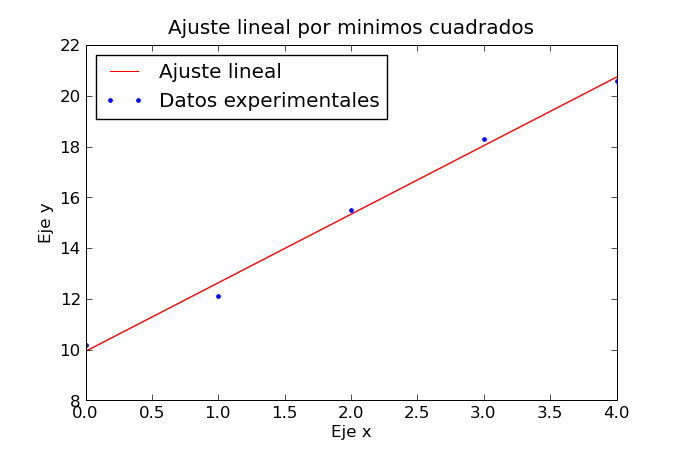
\includegraphics[width=10cm]{plot_ajuste_lineal.png}\hfill}

Como se ve en este ejemplo, la salida por defecto de \textbf{polyfit()} es un array con los parámetros del ajuste. Sin embargo, si se pide una salida detalla con el parámetro \emph{full=True} (por defecto \emph{full=False}), el resultado es una tupla con el array de parámetros, el residuo, el rango, los valores singulares y la condición relativa. Nos interesa especialmente el residuo del ajuste, que es la suma cuadrática de todos los resíduos $\sum^n_{i=1}  \lvert y_i - f(x_i)\rvert**2$. Para el ejemplo anterior tendríamos lo siguiente:

\begin{Verbatim}[commandchars=\\\{\}]
\PYG{c}{\# Ajuste a una recta, con salida completa}
\PYG{n}{resultado} \PYG{o}{=} \PYG{n}{polyfit}\PYG{p}{(}\PYG{n}{x}\PYG{p}{,} \PYG{n}{y}\PYG{p}{,} \PYG{l+m+mi}{1}\PYG{p}{,} \PYG{n}{full}\PYG{o}{=}\PYG{n+nb+bp}{True}\PYG{p}{)}

\PYG{k}{print}\PYG{p}{(}\PYG{n}{resultado}\PYG{p}{)}
\PYG{l+s+sd}{""" Imprime tupla}
\PYG{l+s+sd}{(array([ 2.7 ,  9.94]),                 \# Parámetros del ajuste}
\PYG{l+s+sd}{ array([ 0.472]),                       \# Suma de residuos}
\PYG{l+s+sd}{ 2,                                     \# Rango de la matriz del sistema}
\PYG{l+s+sd}{ array([ 2.52697826,  0.69955764]),     \# Valores singulares}
\PYG{l+s+sd}{ 1.1102230246251565e-15)                \# rcond}
\PYG{l+s+sd}{ """}
\end{Verbatim}

Si estamos trabajando con polinomios, puede que nos interese usar las funciones \textbf{polyval()} o \textbf{poly1d()} de numpy. Se utilizan para evaluar y generar funciones polinómicas respectivamente, a partir de una lista u array de parámetros. Por ejemplo, si del ejemplo anterior tenemos un array \emph{p} con los parámetros del ajuste lineal:

\begin{Verbatim}[commandchars=\\\{\}]
\PYG{c}{\# Evaluo el polinomio en x=5.4}
\PYG{k}{print} \PYG{n}{polyval}\PYG{p}{(}\PYG{n}{p}\PYG{p}{,} \PYG{l+m+mf}{5.4}\PYG{p}{)}
\PYG{c}{\# Imprime 24.520000000000003}

\PYG{c}{\# Creo una funcion polinomica de parametros p}
\PYG{n}{mi\PYGZus{}recta} \PYG{o}{=} \PYG{n}{poly1d}\PYG{p}{(}\PYG{n}{p}\PYG{p}{)}

\PYG{c}{\# Ahora mi\PYGZus{}recta es una funcion que puedo evaluar}

\PYG{c}{\# Evaluo la fucion en x=5.4}
\PYG{k}{print} \PYG{n}{mi\PYGZus{}recta}\PYG{p}{(}\PYG{l+m+mf}{5.4}\PYG{p}{)}
\PYG{c}{\# imprime 24.520000000000003}
\end{Verbatim}

Como es de esperar, \textbf{polyfit()} sólo puede ajustar polinomios pero a veces nos gustaría ajustar otras funciones. En muchos casos, sin embargo, es posible linealizar la función con un cambio de variable adecuado y ajustar esta última. Por ejemplo la función
\begin{gather}
\begin{split}y = \frac{b}{x + a}\end{split}\notag
\end{gather}
se puede linealizar a $y'(x) = a'x + b'$ haciendo el cambio
\begin{gather}
\begin{split}y' = \frac{1}{y} \hspace{1cm} a = \frac{a'}{b'}  \hspace{1cm} b = \frac{1}{a'}.\end{split}\notag
\end{gather}
ahora basta con ajustar la recta   $y'(x) = a'x + b'$ y recuperar
los parámetros \emph{a} y \emph{b} de la recta original.

En otros casos en los que no es posible tal cosa, se trataría de hacer ajustes a funciones no polinómicas, aunque esto queda fuera del alcance de este curso. Si tienes interés, consulta la documentación del módulo \textbf{optimize} de \textbf{scipy}. Por ejemplo, puedes  importar la función \textbf{leastsq()} del módulo \textbf{optimize} haciendo \textbf{from scipy.optimize import leastsq}) para hacer ajustes por mínimos cuadrados de funciones arbitrarias, sean lineales o no. Puedes consultar el módulo \textbf{scipy.optimize} ver todos los métodos de optimización disponibles.


\subsection{Ejercicios}
\label{ajustes:ejercicios}\begin{enumerate}
\item {} 
Representar gráficamente los siguientes datos y hacer un ajuste por mínimos cuadrados a un polinomio de grado tres de los datos representando la curva resultante.
\begin{quote}

\code{x =  3.1   6.3   9.9  12.6   21.4}

\code{y = 50.1 190.2 499.0 720.8 1130.0}
\end{quote}

Superponer los ajuste que resultarían de ajustes a polinomios de orden 1 y 2.

\item {} 
El fichero de texto medidas\_PT\_H.txt (archivos Tema 7) posee medidas de presión y temperatura para 10 mol de hidrógeno, que se somete a distintas temperaturas a volumen constante. Este experimento se realiza en tres envases con volúmenes distintos. Suponiendo que el gas se comporta idealmente y por tanto que se verifica que PV=nRT, representar los datos y realizar un ajuste lineal P(T) para cada volumen. ¿Cuánto vale la constante de gases ideales según el experimento?

\item {} 
El fichero de texto medidas\_PV\_He.txt (archivos Tema 7) posee medidas de presión y volumen para 0.1 mol de helio, que se comprime sistemáticamente a temperatura constante. Este experimento se realiza a tres temperaturas distintas. Suponiendo que el gas se comporta idealmente y por tanto que se verifica que PV=nRT, representar los datos y realizar un ajuste lineal P(V) para cada temperatura. ¿Cuánto vale la constante de gases ideales según el experimento?

\item {} 
Un isótopo radioactivo sigue una ley de desintegración exponencial de la forma $N(t) = N_0e^{-kt}$, donde $N(t)$ es la cantidad de material que queda en un tiempo \emph{t}, $N_0$ la cantidad original (en \emph{t=0}) y \emph{k} es la tasa de decaimiento del isótopo. La semivida de un isótopo es el tiempo que tarda una muestra de ese elemento en disminuir hasta la mitad, es decir $N(T)=N_0/2$.

En un laboratorio se mide cada 12 minutos la masa en gramos de cierto elemento radioactivo. Estos datos se encuentran en el fichero medidas\_sustancia\_radioactiva.txt (archivos Tema 7). Representar gráficamente las medidas con punto y hacer un ajuste por mínimos cuadrados del modelo teórico de desintegración radioactiva para conocer la tasa de decaimiento del isótopo.

\item {} 
Para una muestra que contiene 10g de yodo 131 (semivida de 8 días), se hacen diariamente cinco medidas independientes a lo largo de 60 días. Esas medidas están en el fichero medidas\_decaimiento\_yodo131b.txt (archivos Tema 7), donde cada fila corresponde a cada una de las 5 medidas realizadas diariamente en gramos de yodo que queda. Representar en un gráfico con puntos las cinco medidas con colores distinto para cada una y ajustar a cada una la curva teórica de decaimiento. Imprimir por pantalla los parámetros de cada uno de los cinco ajustes.

\item {} 
Cualquier metal de longitud $L_0$ a temperatura inicial $T0$, que es sometido posteriomente a una temperatura \emph{T} sufre una dilatación o contración dada aproximadamente por $\delta L = \alpha \Delta T)$ donde $\Delta T$ es la diferencia de temperaturas y $\alpha$ el coeficiente de dilatación característico del metal.

En un laboratorio se mide la dilatación que experimentan cuatro varillas de metal de distinto material de longitud inicial $L_0=10cm$ al ir aumentando progresivamente su temperatura en un grado; estos datos se encuentran en el fichero medidas\_dilatacion\_metales.txt. Representar gráficamente las medidas en una única figura con un color distinto para cada metal y calcular el factor de dilatación \emph{a} para cada uno ajustando el modelo teórico a los datos.

\end{enumerate}


\chapter{Cálculo Numérico}
\label{calculo_numerico:calculo-numerico}\label{calculo_numerico::doc}
Aunque el paquete \code{Numpy} ofrece ciertas funcionalidades matemáticas además de la manipulación básica de arrays, como el paquete \code{linalg} para álgebra lineal y \code{random} para números aleatorios, en \code{Scipy} encontraremos todas las herramientas matemáticas que podamos necesitar. \code{Scipy} es una colección de paquetes de algoritmos y herramientas matemáticas para distintas tareas, que también utiliza \code{Numpy}. \code{Scipy} posee varios subpaquetes que deben importarse independientemente cuando se vayan a utilizar; éstos son algunos de ellos:

\begin{tabulary}{\linewidth}{|L|L|}
\hline
\textbf{
Subpaquete
} & \textbf{
Descripción
}\\
\hline

odr
 & 
Regresión de distancias ortogonales (ODR)
\\

misc
 & 
Funciones varias (lectura de imagenes, factorial, etc.)
\\

fftpack
 & 
Algoritmos para transformada de Fourier discreta
\\

io
 & 
Entrada y salida de datos
\\

stats
 & 
Funciones estadisticas
\\

lib
 & 
Envoltorios (\emph{wrappers}) de Python a librerías externas
\\

integrate
 & 
Integración numérica
\\

ndimage
 & 
Imagenes n-dimensionales
\\

linalg
 & 
Álgebra lineal
\\

interpolate
 & 
Herramientas de interpolación
\\

optimize
 & 
Herramientas de optimización
\\

signal
 & 
Tratamiento de señales
\\
\hline
\end{tabulary}


Para ver la lista completa de subpaquetes consultar la ayuda de scipy como \code{help(scipy)()} (haciendo antes \code{import scipy} para tener todos los nombres asociados a \code{scipy}) y consultar su página web para ver la documentación completa (\emph{Link www.scipy.org}). Una manera práctica de trabajar es importar el espacio de nombres de \code{scipy}, es decir el nombre de sus paquetes y funciones principales y luego importar el o los paquetes que vaya a usar, como en este ejemplo:

\begin{Verbatim}[commandchars=\\\{\}]
\PYG{g+gp}{\textgreater{}\textgreater{}\textgreater{} }\PYG{k+kn}{from} \PYG{n+nn}{scipy} \PYG{k+kn}{import} \PYG{o}{*}         \PYG{c}{\# importa el nombre de los subpaquetes únicamente}
\PYG{g+gp}{\textgreater{}\textgreater{}\textgreater{} }\PYG{k+kn}{import} \PYG{n+nn}{optimize}\PYG{o}{,} \PYG{n+nn}{stats}      \PYG{c}{\# importa los paquete optimize y stats}
\end{Verbatim}


\section{Integración numérica}
\label{calculo_numerico:integracion-numerica}
El subpaquete \code{integrate} ofrece varias herramientas de integración numérica con distintos métodos. Podemos ver todos los disponibles consultando su ayuda:

\begin{Verbatim}[commandchars=\\\{\}]
\PYG{g+gp}{\textgreater{}\textgreater{}\textgreater{} }\PYG{k+kn}{from} \PYG{n+nn}{scipy} \PYG{k+kn}{import} \PYG{o}{*}
\PYG{g+gp}{\textgreater{}\textgreater{}\textgreater{} }\PYG{n}{help}\PYG{p}{(}\PYG{n}{integrate}\PYG{p}{)}

\PYG{g+go}{Integration routines}
\PYG{g+go}{====================}

\PYG{g+go}{Methods for Integrating Functions given function object.}

\PYG{g+go}{quad          -- General purpose integration.}
\PYG{g+go}{dblquad       -- General purpose double integration.}
\PYG{g+go}{tplquad       -- General purpose triple integration.}
\PYG{g+go}{fixed\PYGZus{}quad    -- Integrate func(x) using Gaussian quadrature of order n.}
\PYG{g+go}{quadrature    -- Integrate with given tolerance using Gaussian quadrature.}
\PYG{g+go}{romberg       -- Integrate func using Romberg integration.}

\PYG{g+go}{Methods for Integrating Functions given fixed samples.}

\PYG{g+go}{trapz         -- Use trapezoidal rule to compute integral from samples.}
\PYG{g+go}{cumtrapz      -- Use trapezoidal rule to cumulatively compute integral.}
\PYG{g+go}{simps         -- Use Simpson's rule to compute integral from samples.}
\PYG{g+go}{romb          -- Use Romberg Integration to compute integral from}
\PYG{g+go}{                (2**k + 1) evenly-spaced samples.}

\PYG{g+go}{See the special module's orthogonal polynomials (special) for Gaussian}
\PYG{g+go}{    quadrature roots and weights for other weighting factors and regions.}

\PYG{g+go}{Interface to numerical integrators of ODE systems.}

\PYG{g+go}{odeint        -- General integration of ordinary differential equations.}
\PYG{g+go}{ode           -- Integrate ODE using VODE and ZVODE routines.}
\end{Verbatim}

Existen por ejemplo implementaciones del método del trapecio o el método de Simpsom, ambos métodos simples basados en muestras fijas. Las funciones \code{trapz()} y \code{simps()}, que emplean dichos métodos para al cálculo numérico de integrales, adminten como entrada un array \code{y} de valores a integrar y otro array con la variable independiente \code{x}; si no se incluye un segundo parámetro, el espaciado entre los elementos de \code{y} de 1 por defecto, aunque este valor se puede asignar con el parámetro opcional \code{dx=1}.

Supongamos que queremos integrar numéricamente la función $\sin(x)$ de 0 a $pi$, cuyo valor exacto es 2. Veamos cómo se puede calcular numéricamente con distinto número de muestras:

\begin{Verbatim}[commandchars=\\\{\}]
\PYG{g+gp}{\textgreater{}\textgreater{}\textgreater{} }\PYG{k+kn}{from} \PYG{n+nn}{scipy} \PYG{k+kn}{import} \PYG{n}{integrate}

\PYG{g+gp}{\textgreater{}\textgreater{}\textgreater{} }\PYG{c}{\#  Generamos 5 muestras de la función seno, de 0 a pi}
\PYG{g+gp}{\textgreater{}\textgreater{}\textgreater{} }\PYG{n}{x} \PYG{o}{=} \PYG{n}{linspace}\PYG{p}{(}\PYG{l+m+mi}{0}\PYG{p}{,} \PYG{n}{pi}\PYG{p}{,} \PYG{l+m+mi}{5}\PYG{p}{)}
\PYG{g+gp}{\textgreater{}\textgreater{}\textgreater{} }\PYG{n}{y} \PYG{o}{=} \PYG{n}{sin}\PYG{p}{(}\PYG{n}{x}\PYG{p}{)}

\PYG{g+gp}{\textgreater{}\textgreater{}\textgreater{} }\PYG{c}{\# Integramos el array por el método del trapecio}
\PYG{g+gp}{\textgreater{}\textgreater{}\textgreater{} }\PYG{n}{integrate}\PYG{o}{.}\PYG{n}{trapz}\PYG{p}{(}\PYG{n}{y}\PYG{p}{,}\PYG{n}{x}\PYG{p}{)}
\PYG{g+gp}{\textgreater{}\textgreater{}\textgreater{} }\PYG{l+m+mf}{1.8961188979370398}

\PYG{g+gp}{\textgreater{}\textgreater{}\textgreater{} }\PYG{c}{\# Si aunmentamos el número de muestras,}
\PYG{g+gp}{\textgreater{}\textgreater{}\textgreater{} }\PYG{c}{\# la intragración se acerca más al valor analítico}

\PYG{g+gp}{\textgreater{}\textgreater{}\textgreater{} }\PYG{c}{\#  Generamos 20 muestras de la función seno, de 0 a pi}
\PYG{g+gp}{\textgreater{}\textgreater{}\textgreater{} }\PYG{n}{x} \PYG{o}{=} \PYG{n}{linspace}\PYG{p}{(}\PYG{l+m+mi}{0}\PYG{p}{,} \PYG{n}{pi}\PYG{p}{,} \PYG{l+m+mi}{20}\PYG{p}{)}
\PYG{g+gp}{\textgreater{}\textgreater{}\textgreater{} }\PYG{n}{y} \PYG{o}{=} \PYG{n}{sin}\PYG{p}{(}\PYG{n}{x}\PYG{p}{)}

\PYG{g+gp}{\textgreater{}\textgreater{}\textgreater{} }\PYG{c}{\# Integramos el array por el método del trapecio}
\PYG{g+gp}{\textgreater{}\textgreater{}\textgreater{} }\PYG{n}{integrate}\PYG{o}{.}\PYG{n}{trapz}\PYG{p}{(}\PYG{n}{y}\PYG{p}{,}\PYG{n}{x}\PYG{p}{)}
\PYG{g+gp}{\textgreater{}\textgreater{}\textgreater{} }\PYG{l+m+mf}{1.9954413183201947}

\PYG{g+gp}{\textgreater{}\textgreater{}\textgreater{} }\PYG{c}{\# Integramos por el método de Simpson}
\PYG{g+gp}{\textgreater{}\textgreater{}\textgreater{} }\PYG{n}{integrate}\PYG{o}{.}\PYG{n}{simps}\PYG{p}{(}\PYG{n}{y}\PYG{p}{,}\PYG{n}{x}\PYG{p}{)}
\PYG{g+gp}{\textgreater{}\textgreater{}\textgreater{} }\PYG{l+m+mf}{1.999977188106568}
\end{Verbatim}

{\hfill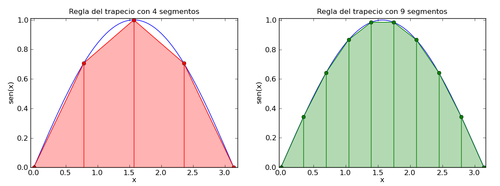
\includegraphics[width=14cm]{plot_trapecio.png}\hfill}

Como se ve, el método de Simpson da un valor más cercano al verdadero, que del trapecio, ya que el primero emplea polinomios de grado 2 para la integración.

En la prática, la función de uso general más eficiente es \code{quad(func, a, b)()}, que integra por cuadratura de Clenshaw-Curtis \footnote{
Para detalles, ver por ejemplo \href{http://en.wikipedia.org/wiki/Clenshaw-Curtis\_quadrature}{http://en.wikipedia.org/wiki/Clenshaw-Curtis\_quadrature}
} una función de Python \code{func()} entre \code{a} y \code{b}. Consideremos como ejemplo el cálculo del área una semicircunferencia de radio unidad calculando la integral bajo la curva. Para ello definimos una función de circunferencia e integramos entre -1 y 1:

La función \code{quad()} devuelve por defecto el valor de la integral, que en este caso vale $\frac{1}{2}\pi$ y una estimación del error en el proceso de integración numérica. Los límites de integración pueden ser $+\infty$ o $-\infty$ usando los símbolos \code{+Inf} o \code{-Inf}:

\begin{Verbatim}[commandchars=\\\{\}]
\PYG{k}{def} \PYG{n+nf}{func1}\PYG{p}{(}\PYG{n}{x}\PYG{p}{)}\PYG{p}{:}
    \PYG{k}{return} \PYG{l+m+mf}{2.0}\PYG{o}{*}\PYG{n}{exp}\PYG{p}{(}\PYG{o}{-}\PYG{n}{x}\PYG{o}{*}\PYG{o}{*}\PYG{l+m+mi}{2}\PYG{o}{/}\PYG{l+m+mf}{5.}\PYG{p}{)}

\PYG{n}{int1}\PYG{p}{,} \PYG{n}{err1} \PYG{o}{=} \PYG{n}{integrate}\PYG{o}{.}\PYG{n}{quad}\PYG{p}{(}\PYG{n}{func1}\PYG{p}{,} \PYG{o}{-}\PYG{l+m+mi}{2}\PYG{p}{,} \PYG{o}{+}\PYG{l+m+mi}{2}\PYG{p}{)}           \PYG{c}{\# integración entre -2 y +2}
\PYG{n}{int2}\PYG{p}{,} \PYG{n}{err2} \PYG{o}{=} \PYG{n}{integrate}\PYG{o}{.}\PYG{n}{quad}\PYG{p}{(}\PYG{n}{func1}\PYG{p}{,} \PYG{o}{-}\PYG{n}{Inf}\PYG{p}{,} \PYG{o}{+}\PYG{n}{Inf}\PYG{p}{)}       \PYG{c}{\# integración entre -infinito y +infinito}

\PYG{k}{print}\PYG{p}{(}\PYG{n}{int1}\PYG{p}{,} \PYG{n}{int2}\PYG{p}{)}
\PYG{p}{(}\PYG{l+m+mf}{6.294530963693763}\PYG{p}{,} \PYG{l+m+mf}{7.9266545952120211}\PYG{p}{)}
\end{Verbatim}

{\hfill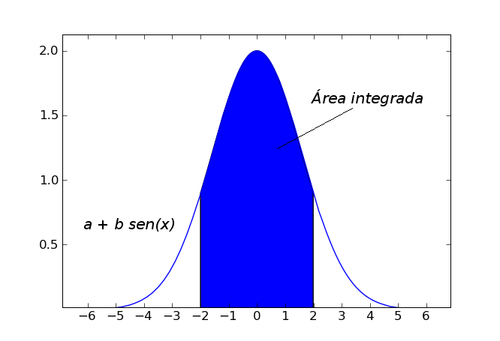
\includegraphics[width=10cm]{integrate_gauss.png}\hfill}

Es posible incluir varios parámetros a la función empleando el parámetro opcional \code{args} como una tupla de parámetros (ver la ayuda de \code{quad()}:

\begin{Verbatim}[commandchars=\\\{\}]
\PYG{c}{\# Definimos la función a integrar, incluyendo parámetros}
\PYG{k}{def} \PYG{n+nf}{f2}\PYG{p}{(}\PYG{n}{x}\PYG{p}{,}\PYG{n}{a}\PYG{p}{,}\PYG{n}{b}\PYG{p}{)}\PYG{p}{:}
     \PYG{k}{return} \PYG{n}{a}\PYG{o}{+} \PYG{n}{b}\PYG{o}{*}\PYG{n}{sin}\PYG{p}{(}\PYG{n}{x}\PYG{p}{)}

\PYG{c}{\# Definimos unos parámetros de entrada}
     \PYG{n}{p}\PYG{o}{=}\PYG{l+m+mf}{0.2}\PYG{p}{;}\PYG{n}{q}\PYG{o}{=}\PYG{l+m+mi}{1}

\PYG{c}{\# Integramos numéricamente, incluyendo parámetros}
\PYG{n}{integrate}\PYG{o}{.}\PYG{n}{quad}\PYG{p}{(}\PYG{n}{f2}\PYG{p}{,} \PYG{l+m+mi}{0}\PYG{p}{,} \PYG{n}{pi}\PYG{p}{,} \PYG{n}{args}\PYG{o}{=}\PYG{p}{(}\PYG{n}{p}\PYG{p}{,}\PYG{n}{q}\PYG{p}{)}\PYG{p}{)}
\PYG{p}{(}\PYG{l+m+mf}{2.6283185307179586}\PYG{p}{,} \PYG{l+m+mf}{2.9180197488520396e-14}\PYG{p}{)}
\end{Verbatim}

Se pueden calcular integrales dobles empleando de manera similar \code{dblquad()}, aunque los límites de la segunda integral se deben poner como funciones de Python.:

\begin{Verbatim}[commandchars=\\\{\}]
\PYG{c}{\# Función a integrar}
\PYG{k}{def} \PYG{n+nf}{f1}\PYG{p}{(}\PYG{n}{x}\PYG{p}{,}\PYG{n}{y}\PYG{p}{)}\PYG{p}{:}
   \PYG{k}{return} \PYG{n}{x}\PYG{o}{+}\PYG{n}{y}

\PYG{c}{\# Límites de la primera integral}
\PYG{n}{a}\PYG{p}{,} \PYG{n}{b} \PYG{o}{=} \PYG{l+m+mi}{0}\PYG{p}{,} \PYG{l+m+mi}{2}

\PYG{c}{\# Definición de limites de segunda integral}
\PYG{k}{def} \PYG{n+nf}{gfun}\PYG{p}{(}\PYG{n}{x}\PYG{p}{)}\PYG{p}{:}
   \PYG{k}{return} \PYG{l+m+mi}{0}

\PYG{k}{def} \PYG{n+nf}{hfun}\PYG{p}{(}\PYG{n}{x}\PYG{p}{)}\PYG{p}{:}
   \PYG{k}{return} \PYG{l+m+mi}{10}

\PYG{n}{integrate}\PYG{o}{.}\PYG{n}{dblquad}\PYG{p}{(}\PYG{n}{f1}\PYG{p}{,} \PYG{l+m+mi}{0}\PYG{p}{,} \PYG{l+m+mi}{2}\PYG{p}{,} \PYG{n}{gfun}\PYG{p}{,} \PYG{n}{hfun}\PYG{p}{)}
\PYG{c}{\# Resultado: (120.00000000000001, 1.3322676295501881e-12)}
\end{Verbatim}


\section{Álgebra matricial}
\label{calculo_numerico:algebra-matricial}
Una maneras de ver \emph{arrays} bidimensionales de \code{Numpy} es como matrices, aunque en realidad los \emph{arrays}, cuando se opera algebraicamente con ellos, no se manipulan como matrices. Por ejemplo el producto de dos arrays bidimensionales \textbf{NxM} se raliza elemento a elemento y no como un producto algebraico de matrices. Veamos unos ejemplos:

\begin{Verbatim}[commandchars=\\\{\}]
\PYG{g+gp}{\textgreater{}\textgreater{}\textgreater{} }\PYG{c}{\# Dos matrices nxn}
\PYG{g+gp}{\textgreater{}\textgreater{}\textgreater{} }\PYG{n}{A} \PYG{o}{=} \PYG{n}{array}\PYG{p}{(}\PYG{p}{[}\PYG{p}{[}\PYG{l+m+mi}{3}\PYG{p}{,} \PYG{l+m+mi}{6}\PYG{p}{,} \PYG{l+m+mi}{7}\PYG{p}{]}\PYG{p}{,} \PYG{p}{[}\PYG{l+m+mi}{2}\PYG{p}{,} \PYG{l+m+mi}{6}\PYG{p}{,} \PYG{l+m+mi}{2}\PYG{p}{]}\PYG{p}{,} \PYG{p}{[}\PYG{l+m+mi}{10}\PYG{p}{,} \PYG{l+m+mi}{9}\PYG{p}{,} \PYG{l+m+mi}{1}\PYG{p}{]}\PYG{p}{]}\PYG{p}{)}
\PYG{g+gp}{\textgreater{}\textgreater{}\textgreater{} }\PYG{n}{B} \PYG{o}{=} \PYG{n}{array}\PYG{p}{(}\PYG{p}{[}\PYG{p}{[}\PYG{l+m+mi}{4}\PYG{p}{,} \PYG{l+m+mi}{5}\PYG{p}{,} \PYG{l+m+mi}{5}\PYG{p}{]}\PYG{p}{,} \PYG{p}{[}\PYG{l+m+mi}{8}\PYG{p}{,} \PYG{l+m+mi}{3}\PYG{p}{,} \PYG{l+m+mi}{4}\PYG{p}{]}\PYG{p}{,} \PYG{p}{[}\PYG{l+m+mi}{3}\PYG{p}{,} \PYG{l+m+mi}{11}\PYG{p}{,} \PYG{l+m+mi}{2}\PYG{p}{]}\PYG{p}{]}\PYG{p}{)}

\PYG{g+gp}{\textgreater{}\textgreater{}\textgreater{} }\PYG{k}{print}\PYG{p}{(}\PYG{n}{A}\PYG{p}{)}
\PYG{g+go}{[[ 3  6  7]}
\PYG{g+go}{ [ 2  6  2]}
\PYG{g+go}{ [10  9  1]]}

\PYG{g+gp}{\textgreater{}\textgreater{}\textgreater{} }\PYG{k}{print}\PYG{p}{(}\PYG{n}{B}\PYG{p}{)}
\PYG{g+go}{[[ 4  5  5]}
\PYG{g+go}{ [ 8  3  4]}
\PYG{g+go}{ [ 3 11  2]]}

\PYG{g+gp}{\textgreater{}\textgreater{}\textgreater{} }\PYG{c}{\# Producto elemento a elemento entre matrices}
\PYG{g+gp}{\textgreater{}\textgreater{}\textgreater{} }\PYG{k}{print}\PYG{p}{(}\PYG{n}{A}\PYG{o}{*}\PYG{n}{B}\PYG{p}{)}
\PYG{g+go}{[[12 30 35]}
\PYG{g+go}{ [16 18  8]}
\PYG{g+go}{ [30 99  2]]}
\end{Verbatim}

Sin embargo \code{Numpy} permite hacer el producto punto entre matrices con la función func:\emph{dot()}:

\begin{Verbatim}[commandchars=\\\{\}]
\PYG{g+gp}{\textgreater{}\textgreater{}\textgreater{} }\PYG{c}{\# Producto punto entre matrices}
\PYG{g+gp}{\textgreater{}\textgreater{}\textgreater{} }\PYG{k}{print}\PYG{p}{(}\PYG{n}{dot}\PYG{p}{(}\PYG{n}{A}\PYG{p}{,}\PYG{n}{B}\PYG{p}{)}\PYG{p}{)}
\PYG{g+go}{[[ 81 110  53]}
\PYG{g+go}{ [ 62  50  38]}
\PYG{g+go}{ [115  88  88]]}
\end{Verbatim}

Si se va a operar a menudo con matrices es conveniente usar el comando \code{mat()} de \code{numpy()}, es una abreviatura de \code{matrix}. Un elemento \code{matrix} es idéntico a un array y se crea de igual manera o a partir de \emph{arrays}, pero se comporta como una matriz:

\begin{Verbatim}[commandchars=@\[\]]
@textgreater[]@textgreater[]@textgreater[] @# Creación elemento matriz (igual que un array)
@textgreater[]@textgreater[]@textgreater[] C = mat(@PYGZlb[]@PYGZlb[]4, 5, 5@PYGZrb[], @PYGZlb[]8, 3, 4@PYGZrb[], @PYGZlb[]3, 11, 2@PYGZrb[]@PYGZrb[])
@textgreater[]@textgreater[]@textgreater[] type(C)
@textgreater[]@textgreater[]@textgreater[] @textless[]class 'numpy.core.defmatrix.matrix'@textgreater[]
@textgreater[]@textgreater[]@textgreater[] @# Conversión de array a matriz
@textgreater[]@textgreater[]@textgreater[] A = mat(A)
@textgreater[]@textgreater[]@textgreater[] type(A)
@textgreater[]@textgreater[]@textgreater[] @textless[]class 'numpy.core.defmatrix.matrix'@textgreater[]
@textgreater[]@textgreater[]@textgreater[] @# Producto matricial
@textgreater[]@textgreater[]@textgreater[] print(A*C)
@PYGZlb[]@PYGZlb[] 81 110  53@PYGZrb[]
 @PYGZlb[] 62  50  38@PYGZrb[]
 @PYGZlb[]115  88  88@PYGZrb[]@PYGZrb[]
\end{Verbatim}


\section{Rutinas básicas con matrices}
\label{calculo_numerico:rutinas-basicas-con-matrices}
La inversa de una matriz $\mathbf{A}$ es una matrix  $\mathbf{B}$ tal que $\mathbf{AB}=\mathbf{I}$ donde  $\mathbf{I}$ es la llamada \textbf{matriz identidad} que consiste en una matriz en la que los elementos en la diagonal son unos y son ceros en el resto. Normalmente  $\mathbf{B}$ se denota como $\mathbf{B}=\mathbf{A}^{-1}$ . En Scipy, la inversa de una matriz de un array Numpy se puede calcular haciendo \code{linalg.inv(A)}, o usando \code{A.I} si A es una matriz. Por ejemplo, consideremos
\begin{gather}
\begin{split}\mathbf{A=}
\left[
        \begin{array}{ccc}
                1 & 3 & 5\\
                2 & 5 & 1\\
                2 & 3 & 8
        \end{array}
\right]\end{split}\notag
\end{gather}
entonces:
\begin{gather}
\begin{split}\mathbf{A^{-1}=\frac{1}{25}\left[\begin{array}{ccc} -37 & 9 & 22\\ 14 & 2 & -9\\ 4 & -3 & 1\end{array}\right]=\left[\begin{array}{ccc} -1.48 & 0.36 & 0.88\\ 0.56 & 0.08 & -0.36\\ 0.16 & -0.12 & 0.04\end{array}\right].}\end{split}\notag
\end{gather}
este cálculo lo haríamos con \code{Scipy} de la siguiente manera:

\begin{Verbatim}[commandchars=\\\{\}]
\PYG{g+gp}{\textgreater{}\textgreater{}\textgreater{} }\PYG{n}{A} \PYG{o}{=} \PYG{n}{mat}\PYG{p}{(}\PYG{p}{[}\PYG{p}{[}\PYG{l+m+mi}{1}\PYG{p}{,} \PYG{l+m+mi}{3}\PYG{p}{,} \PYG{l+m+mi}{5}\PYG{p}{]}\PYG{p}{,} \PYG{p}{[}\PYG{l+m+mi}{2}\PYG{p}{,} \PYG{l+m+mi}{5}\PYG{p}{,} \PYG{l+m+mi}{1}\PYG{p}{]}\PYG{p}{,} \PYG{p}{[}\PYG{l+m+mi}{2}\PYG{p}{,} \PYG{l+m+mi}{3}\PYG{p}{,} \PYG{l+m+mi}{8}\PYG{p}{]}\PYG{p}{]}\PYG{p}{)}
\PYG{g+gp}{\textgreater{}\textgreater{}\textgreater{} }\PYG{n}{A}
\PYG{g+go}{matrix([[1, 3, 5],}
\PYG{g+go}{                  [2, 5, 1],}
\PYG{g+go}{                  [2, 3, 8]])}
\PYG{g+gp}{\textgreater{}\textgreater{}\textgreater{} }\PYG{n}{A}\PYG{o}{.}\PYG{n}{I}
\PYG{g+go}{matrix([[-1.48,  0.36,  0.88],}
\PYG{g+go}{                  [ 0.56,  0.08, -0.36],}
\PYG{g+go}{                  [ 0.16, -0.12,  0.04]])}
\PYG{g+gp}{\textgreater{}\textgreater{}\textgreater{} }\PYG{k+kn}{from} \PYG{n+nn}{scipy} \PYG{k+kn}{import} \PYG{n}{linalg}
\PYG{g+gp}{\textgreater{}\textgreater{}\textgreater{} }\PYG{n}{linalg}\PYG{o}{.}\PYG{n}{inv}\PYG{p}{(}\PYG{n}{A}\PYG{p}{)}
\PYG{g+go}{array([[-1.48,  0.36,  0.88],}
\PYG{g+go}{                 [ 0.56,  0.08, -0.36],}
\PYG{g+go}{                 [ 0.16, -0.12,  0.04]])}
\end{Verbatim}


\section{Resolución de sistemas de ecuaciones lineales}
\label{calculo_numerico:resolucion-de-sistemas-de-ecuaciones-lineales}
Con Scipy es muy fácil resolver un sistema de ecuaciones empleando el comando \code{linalg.solve}. Este comando tiene como parámetros de entrada la matriz y el vector de términos independientes. Si la matriz es simétrica el proceso de cálculo se puede acelerar si se indica como parámetro. Supongamos que queremos resolver el siguiente sistema de ecuaciones:
\begin{gather}
\begin{split}\begin{array}{c c c}
x+3y+5z & = & 10\\
2x+5y+z & = & 8\\
2x+3y+8z & = & 3
\end{array}\end{split}\notag
\end{gather}
Podemos encontrar la solución usando la matriz inversa:
\begin{gather}
\begin{split}\left[\begin{array}{c} x\\ y\\ z\end{array}\right]=\left[\begin{array}{ccc} 1 & 3 & 5\\ 2 & 5 & 1\\ 2 & 3 & 8\end{array}\right]^{-1}\left[\begin{array}{c} 10\\ 8\\ 3\end{array}\right]=\frac{1}{25}\left[\begin{array}{c} -232\\ 129\\ 19\end{array}\right]=\left[\begin{array}{c} -9.28\\ 5.16\\ 0.76\end{array}\right].\end{split}\notag
\end{gather}
Sin embargo, es mejor usar el comando \code{linalg.solve} ya que es más rápido y numéricamente más estable, aunque en este caso el resultado es el mismo:

\begin{Verbatim}[commandchars=\\\{\}]
\PYG{g+gp}{\textgreater{}\textgreater{}\textgreater{} }\PYG{n}{A} \PYG{o}{=} \PYG{n}{mat}\PYG{p}{(}\PYG{l+s}{'}\PYG{l+s}{[1 3 5; 2 5 1; 2 3 8]}\PYG{l+s}{'}\PYG{p}{)}   \PYG{c}{\# Las filas se separan con ";"}
\PYG{g+gp}{\textgreater{}\textgreater{}\textgreater{} }\PYG{n}{b} \PYG{o}{=} \PYG{n}{mat}\PYG{p}{(}\PYG{l+s}{'}\PYG{l+s}{[10;8;3]}\PYG{l+s}{'}\PYG{p}{)}
\PYG{g+gp}{\textgreater{}\textgreater{}\textgreater{} }\PYG{n}{A}\PYG{o}{.}\PYG{n}{I}\PYG{o}{*}\PYG{n}{b}                              \PYG{c}{\# Usando la matriz inversa}
\PYG{g+go}{matrix([[-9.28],}
\PYG{g+go}{                  [ 5.16],}
\PYG{g+go}{                  [ 0.76]])}
\PYG{g+gp}{\textgreater{}\textgreater{}\textgreater{} }\PYG{n}{linalg}\PYG{o}{.}\PYG{n}{solve}\PYG{p}{(}\PYG{n}{A}\PYG{p}{,}\PYG{n}{b}\PYG{p}{)}                   \PYG{c}{\# Usando la funcion {}`{}`linalg.solve(A,b){}`{}`}
\PYG{g+go}{array([[-9.28],}
\PYG{g+go}{                 [ 5.16],}
\PYG{g+go}{                 [ 0.76]])}
\end{Verbatim}


\subsection{Cálculo del determinante}
\label{calculo_numerico:calculo-del-determinante}
Supongamos que  $a_{ij}$ son los elementos de la matriz  $\mathbf{A}$ y  $M_{ij}=\left|\mathbf{A}_{ij}\right|$ será el determinante de la matriz que se obtiene elimiando la \emph{i}-esima fila y la \emph{j}-esima columna de   $\mathbf{A}$. Entonces para cualquier fila \emph{i}:
\begin{gather}
\begin{split}\left|\mathbf{A}\right|=\sum_{j}\left(-1\right)^{i+j}a_{ij}M_{ij}.\end{split}\notag
\end{gather}
Con Scipy el determinante se puede calcular con \textbf{linalg.det}. Por ejemplo, el determinante de la matriz \textbf{A}
\begin{gather}
\begin{split}\mathbf{A=}\left[\begin{array}{ccc} 1 & 3 & 5\\ 2 & 5 & 1\\ 2 & 3 & 8\end{array}\right]\end{split}\notag
\end{gather}
es
\begin{gather}
\begin{split}\begin{array}{ccc} \left|\mathbf{A}\right| & = & 1\left|\begin{array}{cc} 5 & 1\\ 3 & 8\end{array}\right|-3\left|\begin{array}{cc} 2 & 1\\ 2 & 8\end{array}\right|+5\left|\begin{array}{cc} 2 & 5\\ 2 & 3\end{array}\right|\\ & = & 1\left(5\cdot8-3\cdot1\right)-3\left(2\cdot8-2\cdot1\right)+5\left(2\cdot3-2\cdot5\right)=-25.\end{array}\end{split}\notag\\\begin{split}\end{split}\notag
\end{gather}
Con Scipy se calcula tan fácilmente como:

\begin{Verbatim}[commandchars=\\\{\}]
\PYG{g+gp}{\textgreater{}\textgreater{}\textgreater{} }\PYG{n}{A} \PYG{o}{=} \PYG{n}{mat}\PYG{p}{(}\PYG{p}{[}\PYG{p}{[}\PYG{l+m+mi}{1}\PYG{p}{,} \PYG{l+m+mi}{3}\PYG{p}{,} \PYG{l+m+mi}{5}\PYG{p}{]}\PYG{p}{,} \PYG{p}{[}\PYG{l+m+mi}{2}\PYG{p}{,} \PYG{l+m+mi}{5}\PYG{p}{,} \PYG{l+m+mi}{1}\PYG{p}{]}\PYG{p}{,} \PYG{p}{[}\PYG{l+m+mi}{2}\PYG{p}{,} \PYG{l+m+mi}{3}\PYG{p}{,} \PYG{l+m+mi}{8}\PYG{p}{]}\PYG{p}{]}\PYG{p}{)}
\PYG{g+gp}{\textgreater{}\textgreater{}\textgreater{} }\PYG{n}{linalg}\PYG{o}{.}\PYG{n}{det}\PYG{p}{(}\PYG{n}{A}\PYG{p}{)}
\PYG{g+go}{-25.000000000000004}
\end{Verbatim}


\subsection{Ejercicios}
\label{calculo_numerico:ejercicios}\begin{enumerate}
\item {} 
Calcular numéricamente las siguientes integrales
\begin{quote}
\begin{gather}
\begin{split}2\pi \int_0^1 x^3 \sqrt{1 + 9x^4}~dx   ~~~~~~~~~~~~   \int_0^{2\pi}e^{-x} \sin{(10x)}~dx\end{split}\notag
\end{gather}\end{quote}

\item {} 
Calcular numéricamente el área más pequeña comprendida entre un círculo $x^2 + y^2 = 25$ y la recta \emph{x=3}.

\item {} 
Escribir un programa en el que dibujen la función $\frac {ln x}{1-x}$ en el intervalo {[}0,5{]}. Calcular el área bajo de la figura formada por los ejes OX, OY y esta curva en el intervalo {[}0,1{]}. Su resultado exacto es $-\pi^2/6$. Calcular los errores absoluto y relativo con el que se ha obtenido el resultado, dando sólo las cifras significativas.

\item {} 
Crear una función que calcule numéricamente la siguiente integral admitiendo parámetros de entrada \emph{m} y \emph{n}:
\begin{quote}
\begin{gather}
\begin{split}\pi \int_0^1 \frac{x^m - x^n}{\ln{x}} dx  = \ln{\frac{m+1}{n+1}}\end{split}\notag
\end{gather}\end{quote}

\item {} 
Resolver el sistema \textbf{AX=B} donde:
\begin{quote}
\begin{gather}
\begin{split}\begin{array}{ccc}
\mathbf{A=}
\left[
\begin{array}{cccc}
1 & 3 & 5 & 7\\
2 & -1 & 3 & 5\\
0 & 0 & 2 & 5\\
-2 & -6 & -6 & 1
\end{array}
\right] & y &
\begin{array}{ccc}
\mathbf{B=}
\left[
\begin{array}{c}
1\\
2 \\
3\\
4
\end{array}
\right]
\end{array}
\end{array}\end{split}\notag
\end{gather}\end{quote}

\end{enumerate}



\renewcommand{\indexname}{Índice}
\printindex
\end{document}
